%==============================================================================
%  CAHIER DES CHARGES - Zümm
%  Système de gestion et de suivi apicole
%  Structure conforme à la méthode Manager-GO
%  (Contexte / Objectifs / Perimetre / Besoins fonctionnels / Budget / Delais)
%==============================================================================
\documentclass[11pt,a4paper]{report}

% ---------- Encodage & langue -------------------------------------------------
\usepackage[utf8]{inputenc}
\usepackage[T1]{fontenc}
\usepackage[french]{babel}
\usepackage{lmodern}
\usepackage{amsmath}

% ---------- Mise en page ------------------------------------------------------
\usepackage[a4paper,margin=2.5cm,headheight=22pt]{geometry}
\usepackage{setspace}
\onehalfspacing
\usepackage{parskip}

% ---------- Tableaux & listes -------------------------------------------------
\usepackage{array}
\usepackage{longtable}
\usepackage{booktabs}
\usepackage{tabularx}
\usepackage{enumitem}
\setlist{nosep,leftmargin=1.4em}

% ---------- Couleurs & style --------------------------------------------------
\usepackage{xcolor}
% ---- Charte "Miel & noir elegant" -------------------------------------------
\definecolor{miel}{HTML}{D4A017}      % or (accents)
\definecolor{mielfonce}{HTML}{B8860B} % or foncé (titres)
\definecolor{grisdoux}{HTML}{F3F2EE}  % gris clair (fond doux)
\definecolor{bleunuit}{HTML}{1C1C1C}  % anthracite (secondaire)

% ---------- Titres ------------------------------------------------------------
\usepackage{titlesec}
\titleformat{\chapter}[display]
  {\normalfont\huge\bfseries\color{mielfonce}}
  {\filright\Large\color{miel}\MakeUppercase{\chaptertitlename}\ \thechapter}{10pt}{\Huge}
\titleformat{\section}
  {\normalfont\Large\bfseries\color{bleunuit}}{\thesection}{1em}{}
\titleformat{\subsection}
  {\normalfont\large\bfseries\color{mielfonce}}{\thesubsection}{1em}{}

% ---------- En-têtes / pieds --------------------------------------------------
\usepackage{fancyhdr}
\pagestyle{fancy}
\fancyhf{}
\fancyhead[L]{\small\textcolor{mielfonce}{Zümm}}
\fancyhead[R]{\small\textcolor{mielfonce}{Cahier des charges}}
\fancyfoot[C]{\small\thepage}
\renewcommand{\headrulewidth}{0.6pt}
\renewcommand{\headrule}{\hbox to\headwidth{\color{miel}\leaders\hrule height \headrulewidth\hfill}}

% ---------- Liens -------------------------------------------------------------
\usepackage[hidelinks,colorlinks=true,linkcolor=mielfonce,urlcolor=miel]{hyperref}

% ---------- Environnement encadré (contraintes/notes) -------------------------
\usepackage{mdframed}
\newmdenv[
  linecolor=miel,linewidth=1pt,
  backgroundcolor=grisdoux,
  roundcorner=4pt,
  innertopmargin=6pt,innerbottommargin=6pt,
  innerleftmargin=8pt,innerrightmargin=8pt
]{encadre}

% ---------- Figures & images -------------------------------------------------
\usepackage{graphicx}
\graphicspath{{images/}}
\usepackage{tikz}
\usetikzlibrary{positioning,arrows.meta,calc,shapes.geometric}
\usepackage{caption}
\captionsetup{font=small,labelfont={bf,color=mielfonce},labelsep=period}

% Colonne largeur fixe centrée
\newcolumntype{C}[1]{>{\centering\arraybackslash}p{#1}}

%==============================================================================
\begin{document}

% ------------------------------- PAGE DE GARDE -------------------------------
\begin{titlepage}
\centering
\vspace*{1.5cm}
{\color{miel}\rule{\linewidth}{2pt}}\\[0.4cm]
{\Huge\bfseries\color{mielfonce} CAHIER DES CHARGES}\\[0.3cm]
{\LARGE\color{bleunuit} Zümm}\\[0.2cm]
{\large\itshape Système de gestion et de suivi apicole}\\[0.4cm]
{\color{miel}\rule{\linewidth}{2pt}}\\[1.2cm]

\begin{tabular}{@{}>{\bfseries\color{mielfonce}}r l@{}}
Projet        & Application de gestion apicole (mini-projet J2EE)\\[4pt]
Type          & Cahier des charges fonctionnel et technique\\[4pt]
Version       & 1.0\\[4pt]
Date          & \today\\[4pt]
Méthode       & Manager-GO - Élaboration d'un CdC\\
\end{tabular}

\vfill
{\large\bfseries Ruche connectée \& tableaux de bord de performance}\\[0.3cm]
{\small Document conforme au plan type : Contexte / Objectifs / Périmètre /\\
Description fonctionnelle des besoins / Enveloppe budgétaire / Délais}
\vspace{1cm}
\end{titlepage}

% ------------------------------- SOMMAIRE -----------------------------------
\tableofcontents
\thispagestyle{fancy}
\clearpage

\section*{Historique des versions}
\addcontentsline{toc}{chapter}{Historique des versions}
\begin{center}
\begin{tabular}{ccp{3cm}p{6.5cm}}
\toprule
\textbf{Version} & \textbf{Date} & \textbf{Auteur} & \textbf{Modifications} \\
\midrule
0.1 & \today & Équipe projet & Structure initiale et transcription du sujet. \\
0.5 & \today & Équipe projet & Référentiel métier apicole et illustrations. \\
1.0 & \today & Équipe projet & Fonctionnalités du marché, exigences anti-défaut, dictionnaire de données, cas d'utilisation, conception UML et plan de tests. \\
\bottomrule
\end{tabular}
\end{center}
\clearpage

%==============================================================================
\chapter{Contexte et définition du problème}
%==============================================================================

\section{Présentation générale}
Le projet \textbf{Zümm} vise à concevoir un système d'information
dédié à la gestion et au suivi des activités apicoles. L'apiculture moderne
repose sur la surveillance régulière de nombreuses ruches, souvent réparties
sur plusieurs sites géographiques et exploitées par différents apiculteurs.
Le suivi de la santé des colonies, de leur productivité et des interventions
de maintenance constitue une charge organisationnelle importante, aujourd'hui
gérée de façon largement manuelle et dispersée.

\section{Problématique}
En l'absence d'un outil centralisé, les exploitants apicoles rencontrent
plusieurs difficultés :
\begin{itemize}
  \item absence de traçabilité structurée des visites et des inspections des ruches
  \item difficulté à planifier et à coordonner le travail des agents apiculteurs
  \item manque de visibilité sur la production (miel, poids) et sur la rentabilité de chaque site ou ruche
  \item détection tardive des anomalies (baisse d'effectif, chute de production, ouverture non planifiée d'une ruche)
  \item impossibilité d'exploiter automatiquement les mesures issues de capteurs hétérogènes.
\end{itemize}

\section{Finalité}
Le système doit apporter une réponse structurée en deux volets complémentaires :
\begin{enumerate}
  \item une \textbf{gestion manuelle} des opérations de manutention, de leur
        planification et de leur suivi (première partie, objet du présent projet)
  \item une \textbf{supervision distante et automatisée} des indicateurs de
        performance, alimentée par des capteurs, destinée à être développée dans
        le cadre d'un projet ultérieur mais dont le système doit anticiper
        l'intégration.
\end{enumerate}

%==============================================================================
\chapter{Objectifs du projet}
%==============================================================================

\section{Objectif principal}
Fournir une application \textbf{multi-niveaux, évolutive et faiblement couplée}
permettant de gérer l'ensemble du cycle de vie des ruches, de leur composition
physique jusqu'au suivi de production, et d'offrir des tableaux de bord d'aide
à la décision aux différents profils d'utilisateurs.

\section{Objectifs spécifiques}
\begin{itemize}
  \item Assurer les opérations \textbf{CRUD} (création, lecture, mise à jour, suppression) sur l'ensemble des entités métier.
  \item Gérer la hiérarchie \emph{fermier / ferme / site / ruche / corps ou hausse / cadre}.
  \item Planifier, approuver et suivre les visites d'inspection des agents apiculteurs.
  \item Produire des \textbf{rapports de visite} structurés et exploitables.
  \item Offrir des \textbf{tableaux de bord} filtrables (calendrier agents × ruches, alertes de production, alertes sanitaires, synthèse financière).
  \item Anticiper l'intégration de mesures \textbf{horodatées et géolocalisées} issues de capteurs à unités hétérogènes.
  \item Garantir \textbf{internationalisation}, \textbf{sécurité} et \textbf{interopérabilité} (services web).
\end{itemize}

\section{Résultats attendus (indicateurs de réussite)}
\begin{itemize}
  \item Support d'au moins \textbf{trois langues} (FR, EN, AR) en version de démonstration.
  \item Détection automatique des dépassements de seuils \textbf{paramétrables} (production, effectif).
  \item Restitution des données de production par ferme, site et ruche sous forme de graphiques.
  \item Exposition d'une API interrogeable par des applications tierces (Excel, etc.).
\end{itemize}

%==============================================================================
\chapter{Périmètre du projet}
%==============================================================================

\section{Domaine couvert}
Le périmètre du présent cahier des charges couvre \textbf{la première partie}
du système : la gestion manuelle des opérations, leur planification et leur
suivi, ainsi que la préparation de l'architecture pour l'intégration future
des indicateurs automatisés.

\section{Modèle métier et règles de gestion}
\begin{longtable}{>{\bfseries}p{3cm} p{11cm}}
\toprule
\textbf{Entité} & \textbf{Règles de gestion} \\
\midrule
\endhead
Fermier   & Peut posséder plusieurs fermes. \\
Ferme     & Peut comporter plusieurs sites d'apiculture. \\
Site      & Contient une ou plusieurs ruches, dispose d'une localisation géographique (latitude, longitude, altitude, date de mise en œuvre, éventuelles dates de déménagement / clôture). Un site peut accueillir des ruches de différents fermiers et de différentes fermes. \\
Ruche     & Composée d'un compartiment de base (socle / corps) et d'au plus \textbf{5} étages d'extension (hausses). \\
Corps / Hausse & Peut accueillir des cadres de cire installés sur des \emph{slots} identifiés. Le socle/corps doit contenir \textbf{au moins 1} cadre, la capacité maximale d'un corps comme d'une hausse est de \textbf{10 cadres}. \\
Cadre     & Occupe un emplacement (slot) unique dans le corps ou la hausse. \\
Agent apiculteur & Réalise les visites et inspections. Une ruche peut être suivie successivement par plusieurs agents, mais elle est sous la responsabilité d'\textbf{un seul agent} à un instant donné. \\
Agent superviseur & Approuve le planning de visite des ruches dont il a la charge. \\
\bottomrule
\end{longtable}

\begin{encadre}[nobreak=true]
\textbf{Contrainte de composition :} 1 ruche = 1 socle/corps obligatoire + 0 à 5 hausses,
chaque corps/hausse = 1 à 10 cadres, un cadre par slot.
\end{encadre}

\begin{figure}[htbp]
\centering
\begin{tikzpicture}[
  every node/.style={font=\small},
  ent/.style={draw=mielfonce,fill=grisdoux,rounded corners=3pt,minimum height=9mm,inner xsep=7pt,thick},
  fl/.style={-{Latex[length=2mm]},mielfonce,thick}
]
\node[ent] (a) {Fermier};
\node[ent,right=7mm of a] (b) {Ferme};
\node[ent,right=7mm of b] (c) {Site};
\node[ent,right=7mm of c] (d) {Ruche};
\node[ent,below=9mm of d] (e) {Corps / Hausse};
\node[ent,left=7mm of e] (f) {Cadre};
\draw[fl] (a)--(b); \draw[fl] (b)--(c); \draw[fl] (c)--(d);
\draw[fl] (d)--(e); \draw[fl] (e)--(f);
\node[font=\scriptsize,mielfonce,above=0.5mm] at ($(a)!0.5!(b)$) {1..n};
\node[font=\scriptsize,mielfonce,above=0.5mm] at ($(b)!0.5!(c)$) {1..n};
\node[font=\scriptsize,mielfonce,above=0.5mm] at ($(c)!0.5!(d)$) {1..n};
\end{tikzpicture}
\caption{Hiérarchie des entités métier du système Zümm.}
\label{fig:hierarchie}
\end{figure}

\begin{figure}[htbp]
\centering
\begin{tikzpicture}[font=\small]
% périmètre du site
\draw[draw=mielfonce,thick,rounded corners=6pt,fill=grisdoux] (0,0) rectangle (11,4.4);
\node[anchor=north west,mielfonce,font=\bfseries] at (0.2,4.25) {Site apicole};
\node[anchor=north west,font=\footnotesize] at (0.2,3.7)
  {latitude / longitude / altitude, date de mise en oeuvre};
% trois ruches installées sur le site
\foreach \x in {0.9,4.3,7.7}{
  \begin{scope}[shift={(\x,0.7)}]
    \fill[miel!30,draw=mielfonce,thick] (0,0) rectangle (1.4,0.6);
    \fill[miel!40,draw=mielfonce,thick] (0,0.6) rectangle (1.4,1.2);
    \fill[mielfonce] (-0.12,1.2)--(1.52,1.2)--(0.7,1.7)--cycle;
    \draw[mielfonce,thick] (-0.1,-0.12) rectangle (1.5,0);
  \end{scope}
}
\node[font=\scriptsize] at (1.6,0.45) {Ruche};
\node[font=\scriptsize] at (5.0,0.45) {Ruche};
\node[font=\scriptsize] at (8.4,0.45) {Ruche};
% ressources externes
\node[anchor=west,font=\footnotesize,align=left] at (11.4,3.2)
  {Ressources\\(nectar / pollen)\\a environ 1 km};
\draw[-{Latex[length=2mm]},mielfonce,dashed] (11,3.0) -- (11.35,3.0);
\node[anchor=west,font=\footnotesize,align=left] at (11.4,1.2)
  {Distances de securite\\100 / 200 / 300 m\\3 a 4 km des cultures\\traitees};
\end{tikzpicture}
\caption{Schéma d'un site apicole : plusieurs ruches géolocalisées et contraintes d'emplacement.}
\label{fig:site}
\end{figure}

\section{Utilisateurs et droits d'accès}
\begin{longtable}{>{\bfseries}p{3.2cm} p{10.8cm}}
\toprule
\textbf{Profil} & \textbf{Rôle et droits} \\
\midrule
\endhead
Fermier / Propriétaire & Consulte les tableaux de bord de production, de rentabilité et de synthèse, décide de la clôture d'un site ou du déplacement de ruches. \\
Agent apiculteur & Réalise les visites, remplit les rapports, exécute les opérations sur les ruches sous sa responsabilité. \\
Agent superviseur & Approuve les plannings de visite des ruches dont il est responsable. \\
Responsable / Manager & Surveille les alertes (chute de production ou d'effectif) et déclenche les inspections imminentes. \\
Administrateur & Gère les paramètres système, les unités de mesure, les seuils et les référentiels. \\
\bottomrule
\end{longtable}

\section{Hors périmètre}
\begin{itemize}
  \item L'acquisition physique et le déploiement matériel des capteurs (projet ultérieur).
  \item L'automatisation temps réel de la collecte des indicateurs (interface prévue mais non implémentée dans cette phase).
\end{itemize}

%==============================================================================
\chapter{Description fonctionnelle des besoins}
%==============================================================================

\section{Gestion des entités (CRUD)}
Le système doit assurer la création, la consultation, la modification et la
suppression de toutes les entités métier : fermiers, fermes, sites, ruches,
corps/hausses, cadres, agents, visites et rapports, dans le respect des règles
de gestion énoncées au chapitre~3.

\section{Planification et suivi des visites}
\begin{itemize}
  \item Les visites sont \textbf{régulières ou irrégulières}, pour des motifs variés :
        inspection sanitaire, peuplement par un nouvel essaim, changement de reine,
        ravitaillement de nourriture, prescription de médicament, subdivision d'essaim,
        ajout de cadre et/ou d'étage d'extension, collecte de cadres de miel,
        évaluation de la production, évaluation de l'effectif et du volume de l'essaim.
  \item Chaque agent suit un \textbf{planning de visite approuvé} par l'agent superviseur de la ruche concernée.
\end{itemize}

\subsection{Rapport de visite}
Chaque visite donne lieu à un rapport contenant : \textbf{date, heure, durée,
raison, constatations, actions prévues, actions effectuées, recommandations},
une évaluation qualitative de l'effectif / du volume de l'essaim, son état de
santé et son niveau de productivité sur une \textbf{échelle de 1 à 3}.

\section{Tableaux de bord}

\subsection{Calendrier / matrice agents × ruches}
Matrice croisant \textbf{agents et ruches}, déclinée par mois, semaine, saison
et année, avec \textbf{filtres} et regroupements par site, par agent et par agent
responsable. Un clic sur une case représentant une visite planifiée affiche un
\textbf{pop-up} résumant ce qui est prévu (date, heure, raison, actions) et, si
la visite est déjà exécutée, ce qui a été réalisé ainsi que la date et l'heure
effectives.

\subsection{Tableau de bord production (fermier / propriétaire)}
Met en évidence les couples \textbf{site × ruche} dont la production (poids) a
dépassé un \textbf{seuil paramétrable}, signalant soit une collecte de miel
imminente, soit une intervention d'extension et/ou de division d'essaim pour
favoriser l'expansion de la colonie.

\subsection{Tableau de bord alertes (responsable)}
Signale les couples \textbf{site × ruche} dont la production ou l'effectif
baissent de façon inhabituelle au-delà d'un seuil paramétrable, déclenchant une
\textbf{alerte} et une inspection imminente.

\subsection{Tableau de bord de synthèse (propriétaire)}
Graphiques, courbes et histogrammes représentant :
\begin{itemize}
  \item la quantité produite par ferme et par site
  \item le nombre d'interventions par ferme, par site et par ruche
  \item le \textbf{retour sur investissement} (rapport coûts / production) pour arbitrer
        le sort de chaque site ou ruche (clôture, déplacement).
\end{itemize}

\section{Indicateurs de performance (volet automatisé : préparation)}
Les mesures sont \textbf{horodatées et géolocalisées}, exprimées dans des unités
\textbf{paramétrables} (internationalisation des systèmes d'unités). Les mesures
d'un même indicateur ne partagent pas nécessairement la même unité, les capteurs
étant hétérogènes. Indicateurs concernés :
\begin{itemize}
  \item poids du cadre, du socle et de l'étage d'extension
  \item température et humidité, à l'intérieur et à l'extérieur de la ruche
  \item effectif des mouvements d'entrée et de sortie des abeilles
  \item niveau de bruit / bourdonnement, intérieur et extérieur
  \item niveau de luminosité, intérieur et extérieur
  \item vitesse et direction du vent à l'extérieur
  \item état d'ouverture de la ruche (intervention, orage, vol, attaque animale, etc.).
\end{itemize}

\subsection{Analyse prédictive et surveillance connectée}
Les solutions de surveillance connectée (precision beekeeping) telles qu'Arnia,
BroodMinder ou BeeHero montrent que l'exploitation avancée des mêmes indicateurs
permet d'anticiper les événements de la colonie. Le modèle de données doit rester
ouvert à ces traitements, prévus pour le volet automatisé.
\begin{itemize}
  \item détection acoustique de l'essaimage 1 à 5 jours à l'avance par analyse de la signature sonore de la colonie
  \item confirmation de la présence de la reine à partir du bourdonnement
  \item détection d'ouverture, de choc ou de basculement de la ruche par accéléromètre (vol, chute, attaque animale), en complément de l'indicateur d'ouverture
  \item orientation de la ruche par boussole électronique
  \item pesée continue par balance pour suivre le flux de nectar et la dynamique de production
  \item analyse dans le cloud par intelligence artificielle des signatures acoustiques pour corréler son et activité de la ruche.
\end{itemize}

\subsection{Protocole d'ingestion des mesures}
Le volet automatisé reste hors périmètre de développement, mais l'interface
d'ingestion est spécifiée dès maintenant pour que le modèle de données et
l'architecture l'anticipent.
\begin{itemize}
  \item \textbf{Transport} : une passerelle terrain transmet les mesures au
        serveur, au choix selon la connectivité, par \textbf{REST sur HTTPS}
        (\texttt{POST /api/mesures}) ou par \textbf{MQTT} (publication sur le
        topic \texttt{zumm/\{rucheId\}/\{indicateur\}}).
  \item \textbf{Format} : \textbf{JSON}, une mesure portant l'identifiant de la
        ruche, le type d'indicateur, la valeur, l'unité, l'horodatage et la
        géolocalisation ; l'envoi par lot est un tableau de mesures.
  \item \textbf{Fréquence} : paramétrable par indicateur (par exemple poids
        toutes les 15 min, température toutes les 5 min, acoustique échantillonnée
        en continu), afin de maîtriser la volumétrie.
  \item \textbf{Robustesse} : ingestion \textbf{asynchrone} par file d'attente ;
        \textbf{idempotence} sur la clé (ruche, indicateur, horodatage) pour
        rejouer sans doublon ; en zone reculée, mise en tampon locale sur la
        passerelle puis synchronisation différée.
  \item \textbf{Sécurité} : passerelle authentifiée (clé ou certificat), canal
        TLS ; rejet des valeurs hors plage physique plausible (garde-fou).
\end{itemize}
\begin{verbatim}
POST /api/mesures        Content-Type: application/json
{
  "rucheId": 42, "typeIndicateur": "TEMPERATURE_INTERNE",
  "valeur": 34.8, "unite": "degC",
  "horodatage": "2026-07-09T14:05:00Z",
  "latitude": 36.806, "longitude": 10.181
}
\end{verbatim}

\subsection{Seuils par défaut et logique d'alerte}
Les seuils sont stockés dans la table \texttt{SEUIL} (paramétrables, chapitre~5).
Les valeurs ci-dessous sont des \textbf{valeurs par défaut de référence}, ancrées
dans le protocole apicole (chapitre~12).
\begin{longtable}{>{\bfseries}p{4.4cm} p{5.2cm} p{4.4cm}}
\toprule
\textbf{Indicateur} & \textbf{Seuil par défaut} & \textbf{Alerte déclenchée} \\
\midrule
\endhead
Température interne (couvain) & \textless\,32\,°C ou \textgreater\,36\,°C & Risque thermique sur le couvain \\
Humidité interne & \textgreater\,80\,\% & Excès d'humidité, risque sanitaire \\
Poids : gain de la hausse & \textgreater\ seuil de production & Collecte de miel imminente \\
Poids : chute soudaine & \textgreater\,1,5\,kg en moins d'1\,h & Essaimage, vol, chute ou attaque \\
Production ou effectif & Baisse relative \textgreater\,20\,\% vs période précédente & Inspection sanitaire imminente \\
Activité entrée/sortie & $\approx$\,0 en journée favorable & Colonie affaiblie ou reine absente \\
État d'ouverture & Ouvert hors visite planifiée & Intrusion ou perturbation \\
Signature acoustique & Motif d'essaimage détecté & Pré-alerte d'essaimage (1 à 5 j) \\
\bottomrule
\end{longtable}
\begin{encadre}
\textbf{Règle d'évaluation :} à chaque mesure, la valeur est convertie vers
l'unité de référence (formule de conversion, §5.3), puis comparée au seuil
paramétrable. Pour limiter les \emph{fausses alertes}, une alerte n'est levée que
si le dépassement \textbf{persiste sur $N$ mesures consécutives} (anti-rebond /
hystérésis). Toute alerte reste une \textbf{aide à la décision} confirmée par le
rapport de visite : l'agent conserve la validation finale.
\end{encadre}

\section{Grille de synthèse des fonctions}
\begin{longtable}{>{\bfseries}p{3.4cm} p{7.6cm} C{2.2cm}}
\toprule
\textbf{Fonction} & \textbf{Description} & \textbf{Priorité} \\
\midrule
\endhead
CRUD entités        & Gestion complète du modèle métier                       & Haute \\
Planning de visites & Planification + approbation par le superviseur           & Haute \\
Rapports de visite  & Saisie structurée des constats et actions               & Haute \\
Calendrier agents×ruches & Matrice filtrable avec pop-up de résumé            & Haute \\
Alertes production  & Détection des dépassements de seuil                     & Haute \\
Alertes sanitaires  & Détection des baisses anormales d'effectif/production   & Haute \\
Synthèse \& ROI     & Graphiques coûts/production, aide à la décision         & Moyenne \\
Indicateurs capteurs & Modèle de données prêt pour l'automatisation            & Moyenne \\
\midrule
\multicolumn{3}{l}{\textit{\color{mielfonce} Exigences anti-défaut (tirées des limites des solutions existantes)}} \\
\midrule
Déploiement autonome & Installation J2EE sans abonnement ni service tiers obligatoire & Haute \\
Mode hors-ligne & Saisie sans connexion et synchronisation différée & Haute \\
Authentification simple & OAuth Google et parcours de saisie terrain rapide & Haute \\
Modularité configurable & Activation des modules par profil via ConfigZumm.ini & Moyenne \\
Portabilité des données & Export CSV et TXT, service web API et sauvegarde, sans verrouillage & Haute \\
Aide contextuelle & Interface simple et cohérente, guidage de l'utilisateur & Moyenne \\
Parité web et mobile & Mêmes fonctions sur tous les supports & Moyenne \\
Internationalisation & Fichier XML FR, EN et AR, extensible à d'autres langues & Haute \\
Ouverture matérielle & Capteurs hétérogènes et unités paramétrables & Moyenne \\
Ingestion asynchrone & Mesures horodatées différées, volet manuel autonome & Moyenne \\
Validation humaine & Seuils paramétrables et confirmation par le rapport de visite & Haute \\
Sécurité des échanges & SSL et certificats X.509, accès authentifiés & Haute \\
Aide à la décision & Alertes indicatives, l'agent conserve la validation finale & Moyenne \\
\bottomrule
\end{longtable}

\section{Fonctionnalités complémentaires inspirées des solutions du marché}
Afin de renforcer l'ergonomie et la valeur d'usage, le système s'inspire des
bonnes pratiques des applications apicoles de référence telles que HiveTracks.
Ces fonctionnalités étendent les besoins déjà décrits sans les remplacer.
\begin{longtable}{>{\bfseries}p{4.2cm} p{7.5cm} C{2.1cm}}
\toprule
\textbf{Fonction} & \textbf{Description} & \textbf{Priorité} \\
\midrule
\endhead
Photos d'inspection & Attacher une ou plusieurs photos à chaque rapport de visite pour un suivi visuel de la colonie et des cadres. & Haute \\
Saisie vocale assistée & Dicter le compte rendu de visite, la transcription alimentant automatiquement les champs du rapport. & Basse \\
Contexte météo & Afficher la météo locale de la semaine à partir de la localisation du site pour éclairer les décisions d'intervention. & Moyenne \\
Carte et rayons de butinage & Positionner les ruches sur une carte et tracer des rayons de butinage (par exemple 1, 2 et 3 km, unités paramétrables) pour visualiser l'environnement accessible aux abeilles. & Moyenne \\
Liste de tâches et rappels & Gérer une liste de tâches et un calendrier de rappels (nourrissement, inspection, statut de la reine) pour ne manquer aucune échéance. & Haute \\
Suivi de la reine & Enregistrer l'historique du statut de la reine (présence, âge, remplacement, marquage) au fil des visites. & Haute \\
Récolte et QR code & Saisir les récoltes de miel et générer un QR code par lot présentant les notes de dégustation, la provenance et les photos, pour la traçabilité et la valorisation. & Moyenne \\
Accès multi-supports & Offrir un accès web et une expérience adaptée aux terminaux mobiles pour la saisie terrain. & Moyenne \\
\bottomrule
\end{longtable}
\begin{encadre}
\textbf{Cohérence avec les exigences :} les rayons de butinage et la météo
réutilisent la géolocalisation des sites et le mécanisme d'unités paramétrables.
Les rappels s'appuient sur le planning de visite existant, et le suivi de la
reine enrichit le rapport de visite déjà défini.
\end{encadre}

\section{Fonctions de gestion avancée (inspiration Apiary Book et BeePlus)}
Les applications de gestion apicole Apiary Book et BeePlus mettent en avant des
fonctions d'organisation et de traçabilité qui complètent le périmètre du
système.
\begin{longtable}{>{\bfseries}p{4.2cm} p{7.5cm} C{2.1cm}}
\toprule
\textbf{Fonction} & \textbf{Description} & \textbf{Priorité} \\
\midrule
\endhead
Mode hors-ligne et synchronisation & Saisir les données terrain sans connexion et les synchroniser automatiquement au retour du réseau. & Haute \\
Suivi des traitements & Conserver l'historique des médicaments et traitements sanitaires appliqués à chaque ruche. & Haute \\
Gestion du matériel et inventaire & Suivre le matériel (corps, hausses, cadres, ruches) et son affectation aux sites. & Moyenne \\
Suivi financier & Enregistrer coûts et revenus par ferme, site et ruche, en appui du calcul du retour sur investissement. & Moyenne \\
Export des données & Exporter les enregistrements aux formats CSV et TXT pour une analyse externe. & Moyenne \\
Détection de maladies & Aider à l'identification des maladies à partir des constatations de visite. & Basse \\
Sauvegarde des données & Sauvegarder et restaurer les données dans le cloud. & Moyenne \\
\bottomrule
\end{longtable}
\begin{encadre}
\textbf{Cohérence avec les exigences :} le suivi financier alimente le tableau de
bord de retour sur investissement, l'export CSV prolonge le service web API, et
le suivi des traitements enrichit le motif de visite prescription de médicament.
\end{encadre}

\section{Limites connues des solutions existantes et exigences pour les éviter}
L'analyse des retours d'expérience sur les solutions du marché (HiveTracks,
Apiary Book, BeePlus) et sur les systèmes de surveillance connectée (Arnia,
BroodMinder, BeeHero) fait ressortir des limites récurrentes. Le tableau suivant
met chaque limite en regard de l'exigence retenue pour l'éviter dans Zümm.
\begin{longtable}{>{\bfseries}p{5.2cm} p{9.3cm}}
\toprule
\textbf{Limite observée} & \textbf{Exigence retenue pour l'éviter} \\
\midrule
\endhead
Abonnement payant et paywall & Système autodéployable en J2EE, sans abonnement obligatoire, l'ensemble des fonctions de gestion reste accessible. \\
Fonctionnement hors-ligne limité & Mode hors-ligne robuste avec synchronisation différée, la saisie terrain n'exige pas de connexion permanente. \\
Création de compte imposée et friction & Authentification simple par OAuth Google et parcours de saisie rapide, l'ergonomie prime. \\
Surcharge de fonctions inutiles & Modules activables par profil et par le fichier de configuration ConfigZumm.ini, grâce à l'architecture faiblement couplée. \\
Dépendance et perte des données & Données maîtrisées par l'utilisateur, export CSV et TXT, service web API et sauvegarde, sans verrouillage propriétaire. \\
Interface dense et courbe d'apprentissage & Interface simple, cohérente et conviviale avec aide contextuelle, conformément aux exigences d'ergonomie. \\
Fonctions inégales selon la plateforme & Parité fonctionnelle entre accès web et mobile grâce à l'architecture multi-niveaux. \\
Solutions uniquement anglophones & Internationalisation par fichier XML, au moins FR, EN et AR, ouverte à d'autres langues. \\
Coût élevé du matériel de capteurs & Ouverture aux capteurs hétérogènes et bon marché avec unités paramétrables, sans verrouillage matériel. \\
Autonomie et connectivité en zone reculée & Ingestion asynchrone de mesures horodatées, le volet manuel fonctionne sans capteurs. \\
Fausses alertes et fiabilité des capteurs & Seuils paramétrables et validation humaine par le rapport de visite, les alertes restent une aide à la décision. \\
Confidentialité et sécurité des données & Chiffrement SSL et certificats X.509, authentification des accès. \\
Surconfiance dans l'automatisation & Positionnement en aide à la décision, l'agent apiculteur conserve la validation finale. \\
\bottomrule
\end{longtable}

%==============================================================================
\chapter{Dictionnaire de données et règles de calcul}
%==============================================================================
Ce chapitre répond à la question des inputs et des outputs du système. Il définit
les données manipulées, leurs types et les formules de calcul des résultats.

\section{Conventions de types}
Les types utilisés sont : entier, décimal, texte, date, heure, datetime, booléen,
énumération et référence (clé étrangère vers une autre entité). Les grandeurs
physiques sont associées à une unité paramétrable pour permettre
l'internationalisation des systèmes de mesure.

\section{Dictionnaire des données (inputs)}
\begin{longtable}{>{\bfseries}p{2.6cm} p{3.4cm} p{2.4cm} p{5cm}}
\toprule
\textbf{Entité} & \textbf{Attribut} & \textbf{Type} & \textbf{Description} \\
\midrule
\endhead
Fermier & id, nom, contact & entier, texte & Propriétaire exploitant. \\
Ferme & id, nom, fermier & entier, texte, référence & Exploitation rattachée à un fermier. \\
Site & id, nom & entier, texte & Emplacement d'apiculture. \\
Site & latitude, longitude & décimal (degrés) & Géolocalisation. \\
Site & altitude & décimal (unité paramétrable) & Altitude du site. \\
Site & dateMiseEnOeuvre, dateDemenagement, dateCloture & date & Cycle de vie du site, deux dernières optionnelles. \\
Ruche & id, modele & entier, texte & Ruche hébergée par un site. \\
Ruche & nbHausses & entier (0 à 5) & Nombre d'étages d'extension. \\
Ruche & ferme & référence & Ferme propriétaire (distincte du site d'emplacement). \\
Ruche & etat & énumération & État du cycle de vie (créée, peuplée, active, en division, en collecte, clôturée), voir figure~\ref{fig:etat}. \\
Ruche & agentResponsable & référence & Agent responsable à l'instant donné. \\
Compartiment & id, type & entier, énumération & Compartiment de la ruche : corps ou hausse. \\
Compartiment & capaciteCadres & entier (1 à 10) & Nombre de slots de cadres. \\
Cadre & id, slot, type & entier, énumération & Cadre installé sur un slot identifié. \\
Cadre & poids & décimal (unité paramétrable) & Poids du cadre, base du calcul de la quantité de miel. \\
Agent & id, nom, role & entier, texte, énumération & Apiculteur, superviseur, responsable ou administrateur. \\
Planning & id, ruche, agent & entier, référence & Planning de visite. \\
Planning & datePrevue, statutApprobation & date, énumération & Date prévue et approbation du superviseur. \\
Planning & superviseur & référence & Agent superviseur qui approuve le planning. \\
Visite & id, ruche, agent & entier, référence & Visite réalisée. \\
Visite & planning & référence & Planning approuvé à l'origine de la visite (optionnel). \\
Visite & date, heure, duree & date, heure, entier (min) & Horodatage et durée. \\
Visite & raison & énumération & Motif de la visite. \\
Visite & constatations, actionsPrevues, actionsEffectuees, recommandations & texte & Contenu du rapport. \\
Visite & effectifQualitatif, etatSante & énumération & Évaluation de l'essaim. \\
Visite & productivite & entier (1 à 3) & Niveau de productivité. \\
Photo & id, url, visite & entier, texte, référence & Photo attachée à un rapport de visite. \\
Mesure & id, ruche, typeIndicateur & entier, référence, énumération & Mesure d'un indicateur. \\
Mesure & valeur, unite & décimal, texte & Valeur et unité paramétrable. \\
Mesure & horodatage, latitude, longitude & datetime, décimal & Mesure horodatée et géolocalisée. \\
Récolte & id, ruche, date & entier, référence, date & Récolte de miel. \\
Récolte & quantiteMiel, lotQR & décimal (unité paramétrable), texte & Quantité et identifiant de lot. \\
Seuil & id, type, valeur, unite & entier, énumération, décimal, texte & Seuil paramétrable du système. \\
\bottomrule
\end{longtable}

\begin{encadre}
\textbf{Schéma de référence :} le dictionnaire ci-dessus est la vue métier des
données. Sa traduction relationnelle normalisée (clés, types SQL et contraintes
\texttt{CHECK}) constitue le \textbf{modèle logique de données} (MLD), qui fait
foi pour l'implémentation et est présenté à l'annexe~\ref{chap:complements}
(figure~\ref{fig:mld}). La correspondance des noms entre le dictionnaire, le
diagramme de classes et le MLD est donnée par la table~\ref{tab:vocabulaire}.
\end{encadre}

\section{Résultats et règles de calcul (outputs)}
\begin{itemize}
  \item \textbf{Quantité de miel d'une ruche} : somme des poids des cadres de miel des hausses, diminuée de la tare des éléments.
\end{itemize}
\[ \text{QuantiteMiel}(r) = \sum_{c \in \text{cadresMiel}(r)} \text{poids}(c) - \text{tare}(r) \]
Cette valeur est exposée par le service web via \texttt{getZummHoneyActualQuantity(zummID)}.
\begin{itemize}
  \item \textbf{Retour sur investissement} d'un site ou d'une ruche :
\end{itemize}
\[ \text{ROI} = \frac{\text{Production valorisée}}{\text{Coûts des interventions}} \]
\begin{itemize}
  \item \textbf{Alerte de collecte} : déclenchée si la production dépasse le seuil paramétrable.
\end{itemize}
\[ \text{Production}(r) > \text{SeuilProduction} \Rightarrow \text{alerte collecte ou extension} \]
\begin{itemize}
  \item \textbf{Alerte de baisse} : déclenchée si la baisse relative dépasse le seuil.
\end{itemize}
\[ \frac{V_{\text{préc}} - V_{\text{actuel}}}{V_{\text{préc}}} > \text{SeuilBaisse} \Rightarrow \text{alerte inspection} \]
\begin{itemize}
  \item \textbf{Conversion d'unités} vers l'unité de référence, pour comparer des mesures hétérogènes :
\end{itemize}
\[ V_{\text{référence}} = V_{\text{mesure}} \times \text{facteurConversion}(\text{unite}) \]

\section{Requêtes types}
Les résultats s'appuient sur des requêtes exécutées via JDBC, par exemple pour la
quantité de miel d'une ruche : \texttt{SELECT SUM(quantiteMiel) FROM recolte WHERE ruche = zummID}.

%==============================================================================
\chapter{Cas d'utilisation détaillés}
%==============================================================================
Cette partie décrit comment le système réalise les opérations des utilisateurs.
Les acteurs sont le fermier, l'agent apiculteur, l'agent superviseur, le
responsable, l'administrateur et les applications tierces.

Le diagramme de cas d'utilisation global (figure \ref{fig:uc}) présente
l'ensemble des acteurs, la généralisation de l'agent superviseur à partir de
l'agent apiculteur, ainsi que toutes les dépendances entre cas (relations
d'inclusion et d'extension).
\begin{figure}[htbp]
\centering
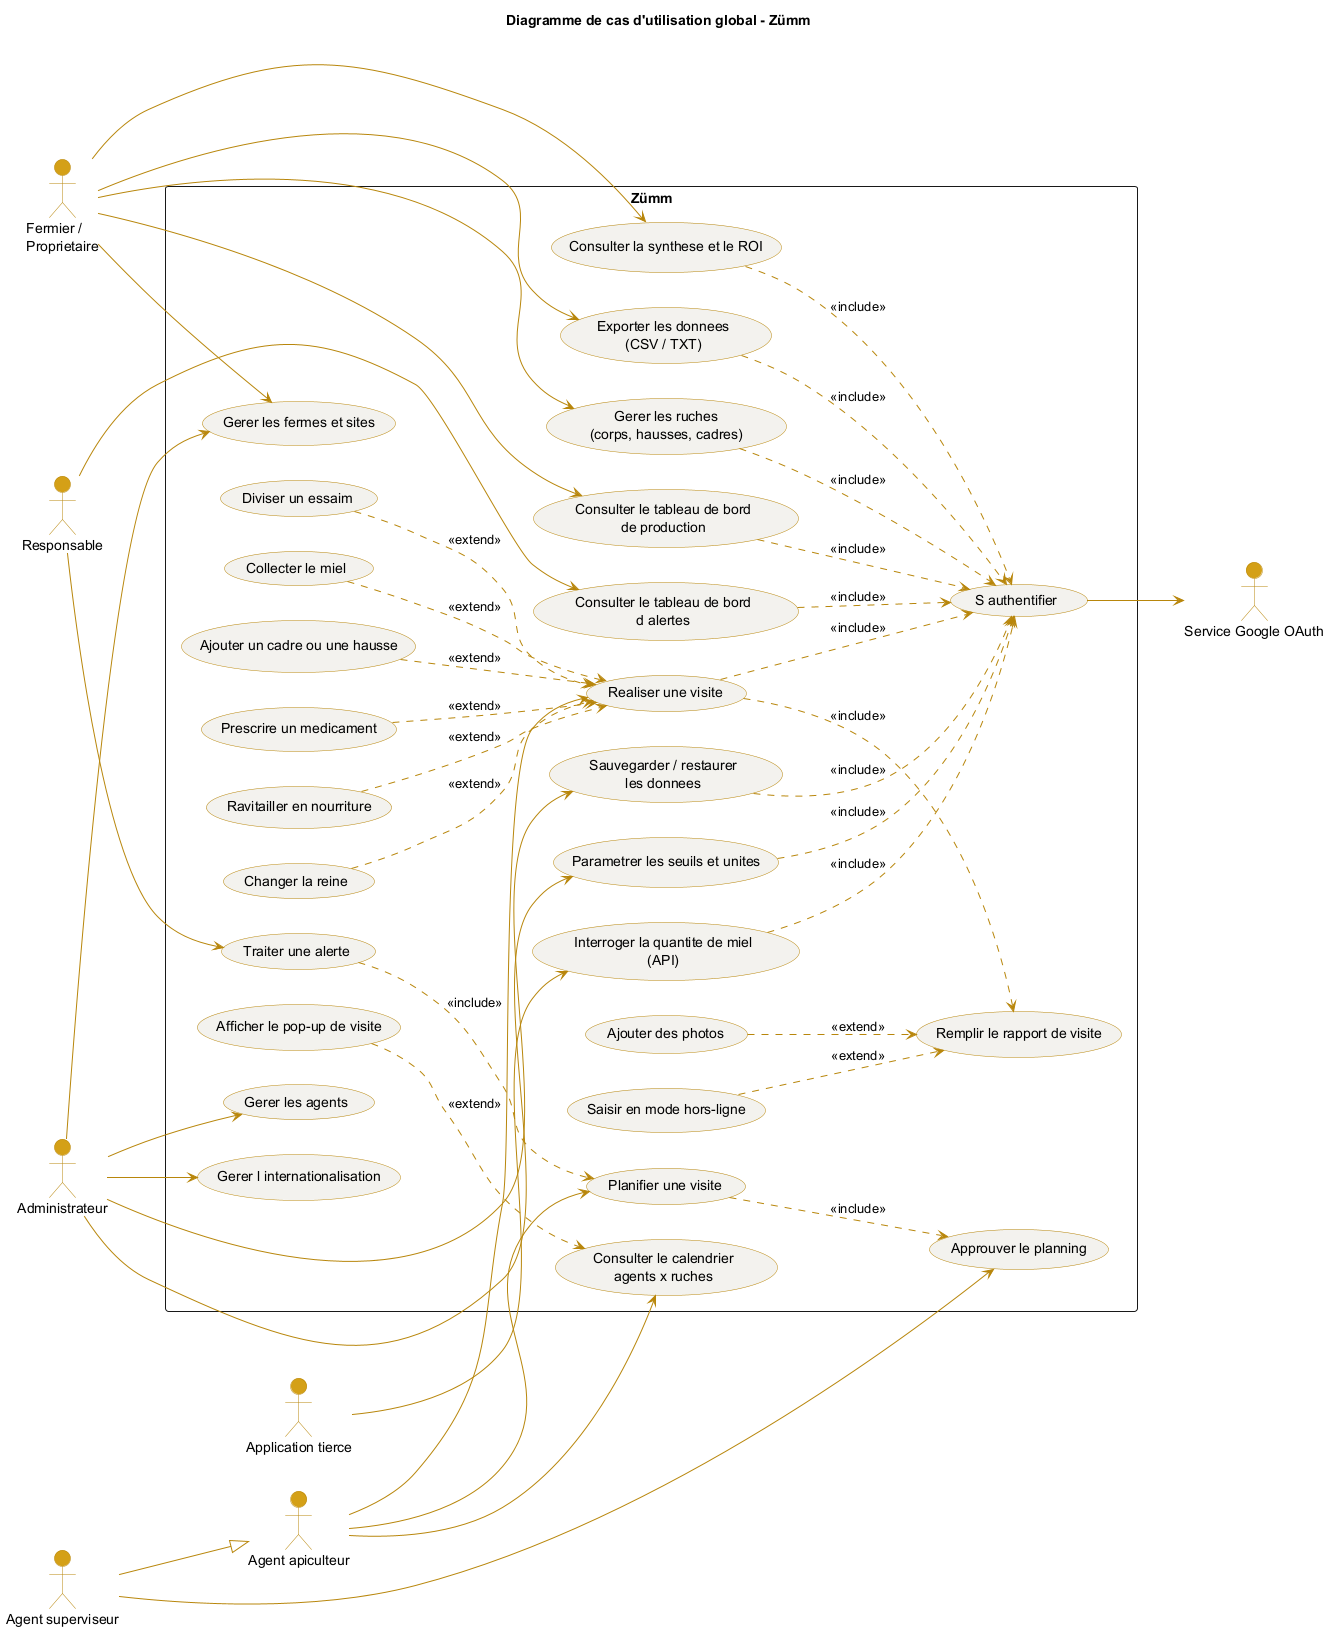
\includegraphics[width=\linewidth]{diagramme_cas_utilisation}
\caption{Diagramme de cas d'utilisation global avec acteurs et dépendances (include et extend).}
\label{fig:uc}
\end{figure}

\section{UC1 : Planifier et approuver une visite}
\begin{itemize}
  \item \textbf{Acteur} : agent superviseur.
  \item \textbf{Préconditions} : la ruche existe et l'agent est authentifié.
  \item \textbf{Scénario nominal} : l'agent propose une date de visite, le superviseur examine le planning puis approuve, le système enregistre le statut approuvé.
  \item \textbf{Alternatives} : le superviseur refuse et demande une nouvelle date.
  \item \textbf{Postcondition} : la visite est planifiée et visible dans le calendrier.
\end{itemize}

\section{UC2 : Réaliser une visite et remplir le rapport}
\begin{itemize}
  \item \textbf{Acteur} : agent apiculteur responsable de la ruche.
  \item \textbf{Préconditions} : une visite est planifiée et approuvée.
  \item \textbf{Scénario nominal} : l'agent renseigne date, heure, durée, raison, constatations, actions prévues et effectuées, recommandations, puis évalue l'effectif, l'état de santé et la productivité de 1 à 3.
  \item \textbf{Alternatives} : saisie hors-ligne puis synchronisation différée, ajout de photos.
  \item \textbf{Postcondition} : le rapport est enregistré et la case du calendrier passe au statut exécuté.
\end{itemize}

\section{UC3 : Consulter le tableau de bord de production}
\begin{itemize}
  \item \textbf{Acteur} : fermier ou propriétaire.
  \item \textbf{Préconditions} : des mesures de production existent.
  \item \textbf{Scénario nominal} : le fermier filtre par ferme, site et période, le système affiche les ruches dont la production dépasse le seuil et propose collecte ou extension.
  \item \textbf{Postcondition} : le fermier décide d'une intervention.
\end{itemize}

\section{UC4 : Traiter une alerte sanitaire}
\begin{itemize}
  \item \textbf{Acteur} : responsable.
  \item \textbf{Préconditions} : une baisse anormale a été détectée.
  \item \textbf{Scénario nominal} : le système signale la ruche concernée, le responsable planifie une inspection imminente.
  \item \textbf{Postcondition} : une visite d'inspection est planifiée.
\end{itemize}

\section{UC5 : Interroger la quantité de miel via l'API}
\begin{itemize}
  \item \textbf{Acteur} : application tierce (Excel ou autre).
  \item \textbf{Préconditions} : l'application dispose d'un accès sécurisé au service web.
  \item \textbf{Scénario nominal} : l'application appelle \texttt{getZummHoneyActualQuantity(zummID)}, le service calcule et retourne la quantité de miel.
  \item \textbf{Postcondition} : la valeur est restituée au format du service web XML.
\end{itemize}

%==============================================================================
\chapter{Conception (modèles UML)}
\label{chap:conception}
%==============================================================================
Le dossier de conception comprend les diagrammes UML suivants. Chacun est décrit
par son contenu attendu afin de guider la modélisation.
\begin{longtable}{>{\bfseries}p{3.8cm} p{10.2cm}}
\toprule
\textbf{Diagramme} & \textbf{Contenu attendu} \\
\midrule
\endhead
Cas d'utilisation & Acteurs (fermier, agent, superviseur, responsable, administrateur, application tierce) et cas principaux (voir figure \ref{fig:uc}). \\
Classes & Entités du dictionnaire de données et leurs relations (Fermier 1 vers n Ferme, Ferme 1 vers n Site, Site 1 vers n Ruche, Ruche 1 vers n Corps ou hausse, Corps ou hausse 1 vers n Cadre) et méthodes de service. \\
Objets & Instantané d'un site contenant trois ruches peuplées avec leurs cadres. \\
Séquence & Déroulé de la réalisation d'une visite (Agent, IHM JSP, Servlet, EJB, JDBC, base de données). \\
Activité & Processus de planification, approbation, exécution et clôture d'une visite. \\
Machine à états & Cycle de vie d'une ruche (créée, peuplée, active, en division, en collecte, clôturée). \\
Interaction ou collaboration & Même scénario que la séquence sous forme de collaboration entre objets. \\
Package & Couches présentation, contrôle, métier, accès aux données, internationalisation, configuration et services web. \\
Composant & Composants applicatifs (application web, service OAuth, service API, module i18n, module configuration, base de données). \\
Déploiement & Répartition sur le navigateur, le serveur d'applications J2EE, le SGBD, le service Google OAuth et les capteurs. \\
\bottomrule
\end{longtable}

\section{Diagramme de classes}
Le diagramme de classes, présenté en alignement horizontal, décrit les entités
métier, leurs attributs, la méthode de service \texttt{getZummHoneyActualQuantity}
et les relations avec leurs cardinalités.
\begin{figure}[htbp]
\centering
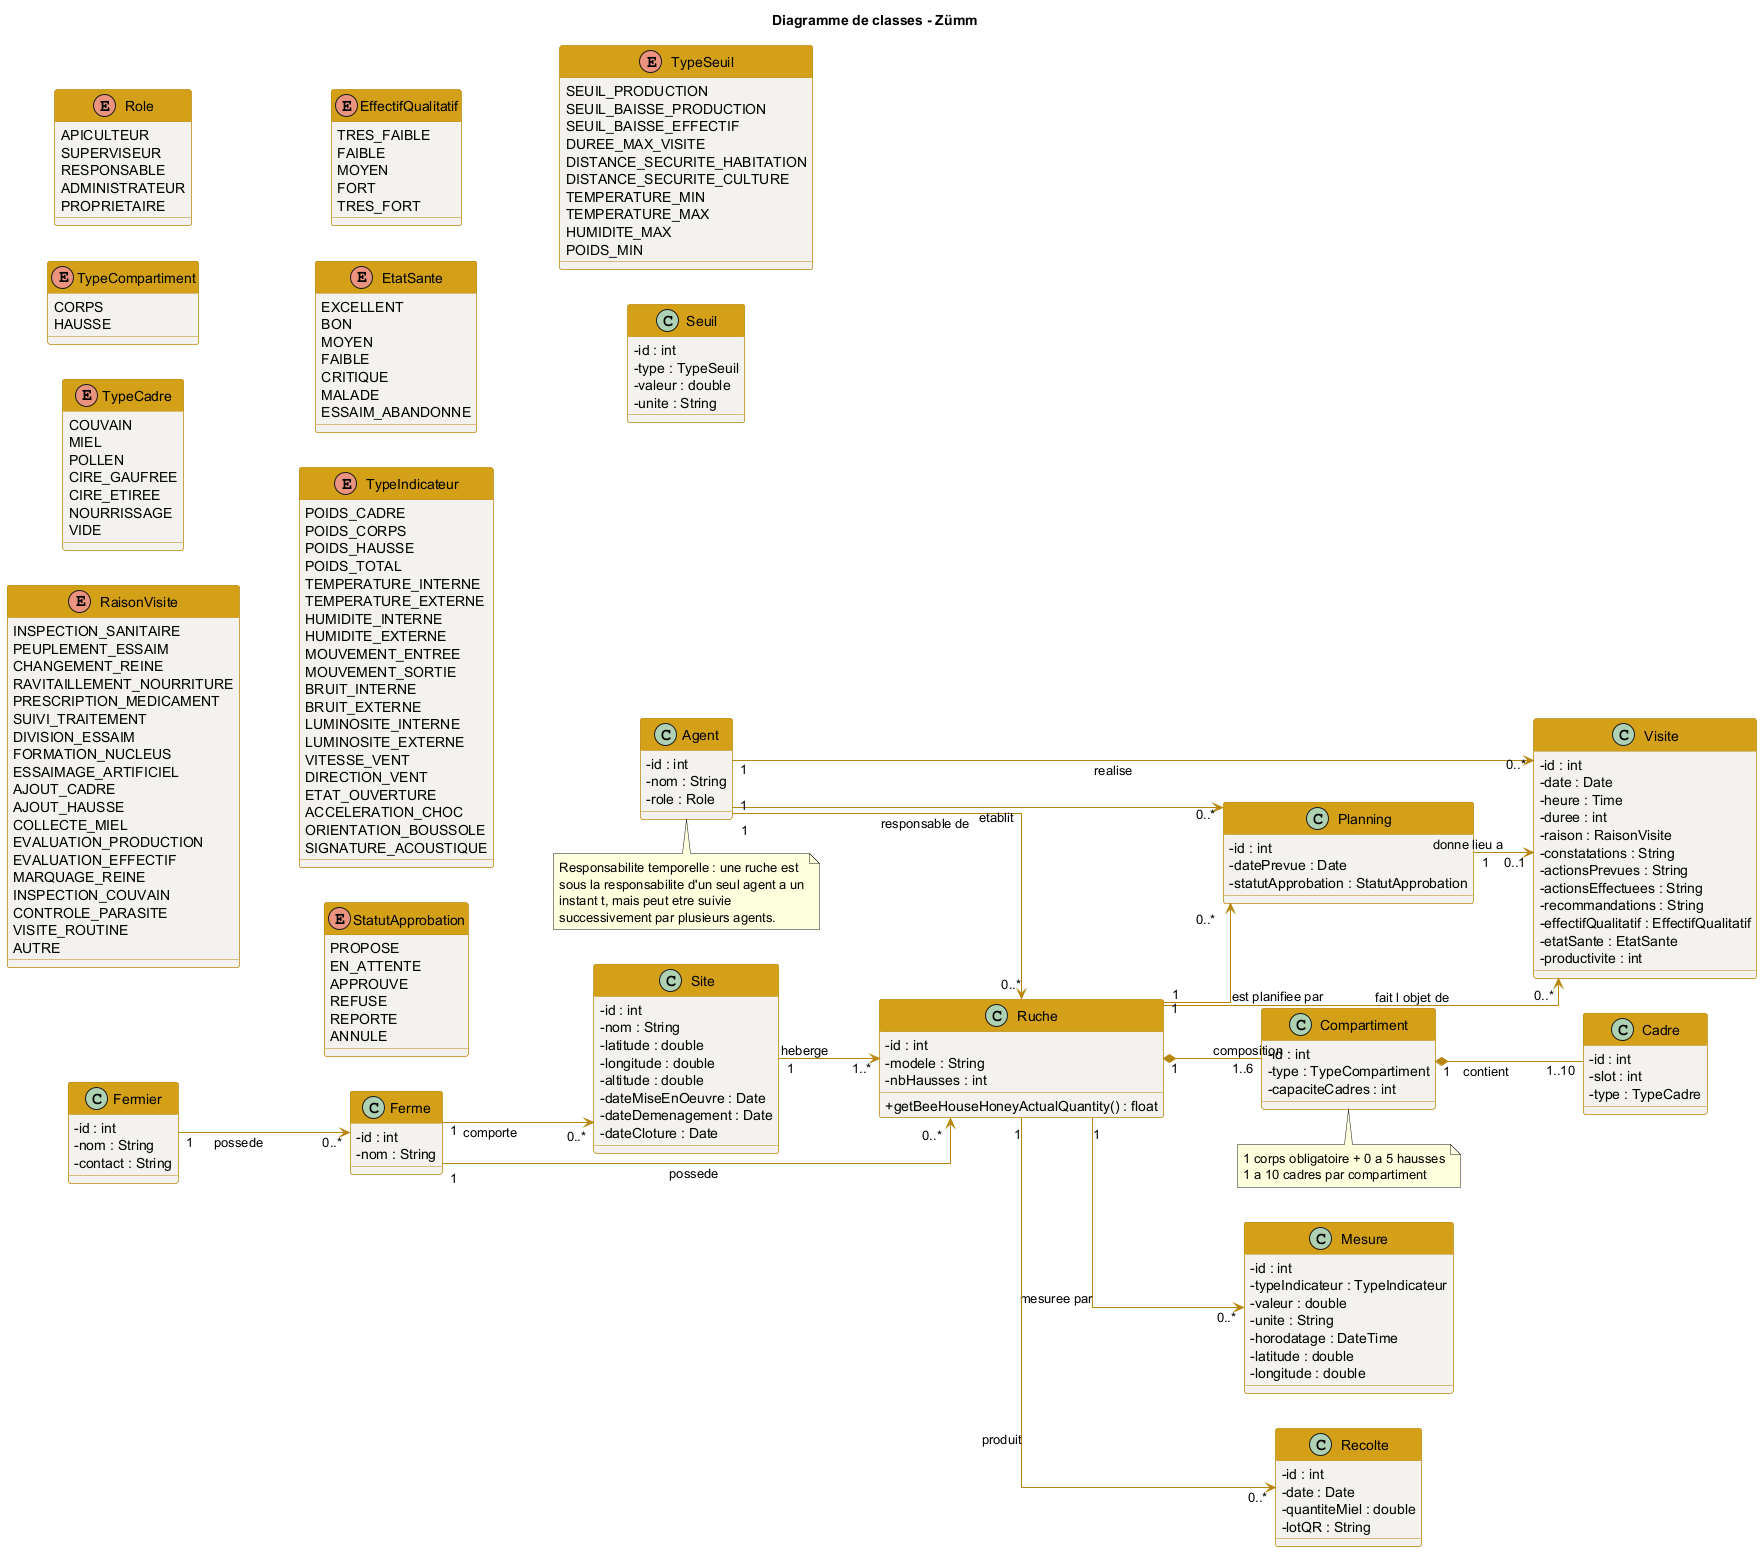
\includegraphics[width=\linewidth]{diagramme_classes}
\caption{Diagramme de classes du système Zümm (alignement horizontal).}
\label{fig:classes}
\end{figure}

\section{Vue en couches (package)}
\begin{figure}[htbp]
\centering
\begin{tikzpicture}[
  couche/.style={draw=mielfonce,fill=grisdoux,thick,minimum width=10cm,minimum height=8mm,font=\small}
]
\node[couche] (p) at (0,4) {Présentation : JSP et JavaScript};
\node[couche] (c) at (0,3) {Contrôle : Servlets (MVC)};
\node[couche] (m) at (0,2) {Métier : EJB};
\node[couche] (d) at (0,1) {Accès aux données : JDBC};
\node[couche] (b) at (0,0) {Base de données relationnelle};
\node[draw=mielfonce,thick,fill=miel!15,minimum height=8mm,font=\footnotesize,right=3mm of c,xshift=4.7cm] (s) {i18n XML / ConfigZumm.ini / Services web};
\draw[-{Latex[length=2mm]},mielfonce] (p)--(c);
\draw[-{Latex[length=2mm]},mielfonce] (c)--(m);
\draw[-{Latex[length=2mm]},mielfonce] (m)--(d);
\draw[-{Latex[length=2mm]},mielfonce] (d)--(b);
\end{tikzpicture}
\caption{Architecture multi-niveaux en couches faiblement couplées.}
\label{fig:couches}
\end{figure}

\section{Vue de déploiement}
\begin{figure}[htbp]
\centering
\begin{tikzpicture}[
  noeud/.style={draw=mielfonce,fill=grisdoux,thick,minimum width=3cm,minimum height=1.1cm,font=\footnotesize,align=center},
  fl/.style={-{Latex[length=2mm]},mielfonce,thick}
]
\node[noeud] (nav) {Navigateur\\(client web)};
\node[noeud,right=1.6cm of nav] (srv) {Serveur J2EE\\(Servlets, EJB)};
\node[noeud,right=1.6cm of srv] (bd) {SGBD\\relationnel};
\node[noeud,below=1cm of srv] (oauth) {Google OAuth};
\node[noeud,below=1cm of bd] (capt) {Capteurs\\(volet automatisé)};
\draw[fl] (nav)--(srv) node[midway,above,font=\scriptsize]{HTTPS};
\draw[fl] (srv)--(bd) node[midway,above,font=\scriptsize]{JDBC};
\draw[fl] (srv)--(oauth) node[midway,right,font=\scriptsize]{SSL};
\draw[fl] (capt)--(srv);
\end{tikzpicture}
\caption{Diagramme de déploiement du système.}
\label{fig:deploiement}
\end{figure}

\section{Diagramme de séquence (UC2)}
Le diagramme de séquence ci-dessous détaille le cas d'utilisation UC2, réaliser
une visite et remplir le rapport. Il montre le passage à travers les couches
(agent, IHM, servlet, EJB, base de données) ainsi que les cas en ligne et
hors-ligne avec synchronisation différée.
\begin{figure}[htbp]
\centering
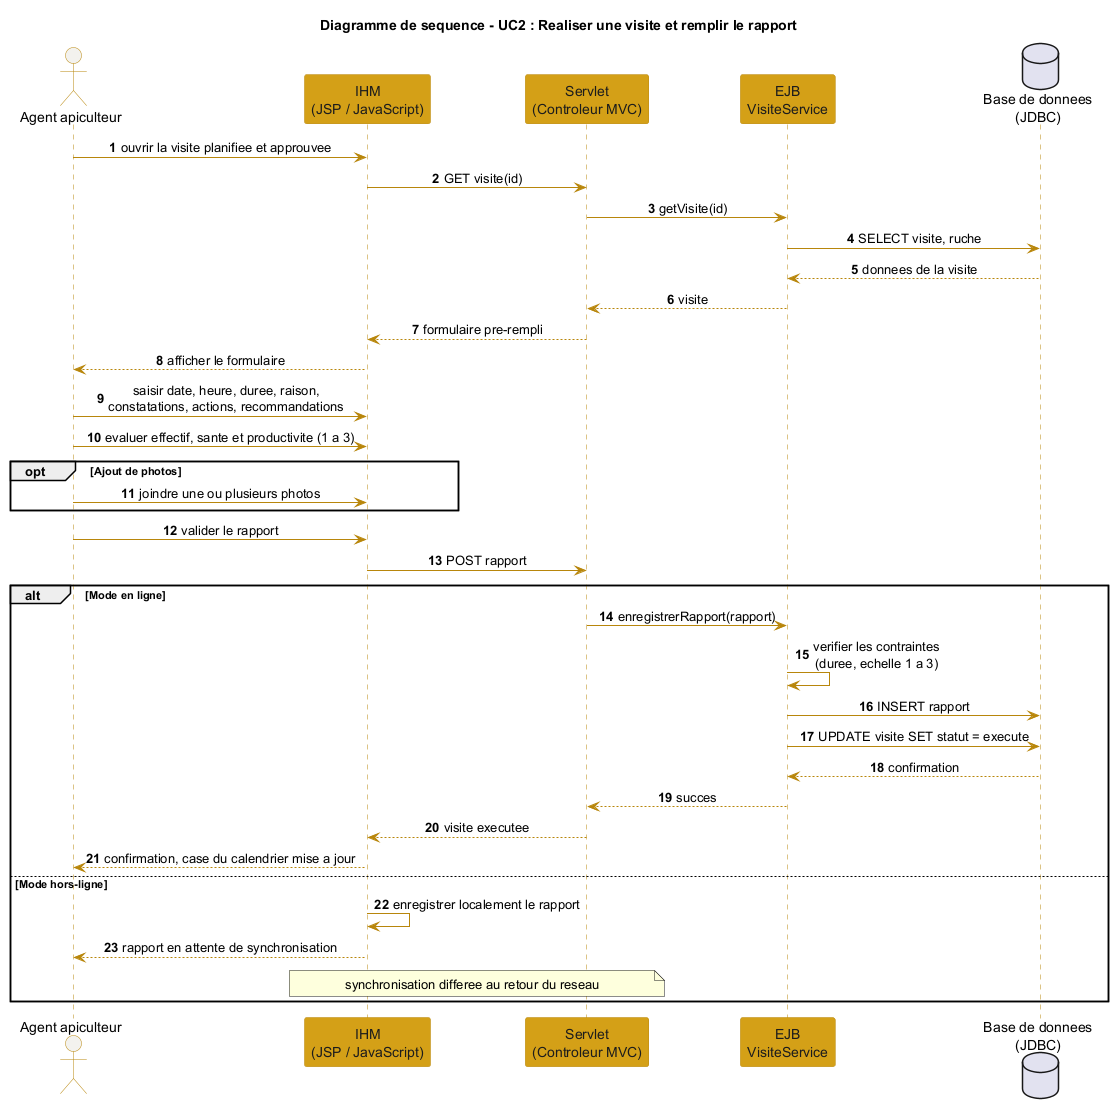
\includegraphics[width=0.92\linewidth]{diagramme_sequence_uc2}
\caption{Diagramme de séquence du cas d'utilisation UC2 (réaliser une visite).}
\label{fig:sequence-uc2}
\end{figure}

\section{Séquence d'authentification (OAuth Google)}
Le parcours d'authentification suit le flot \emph{Authorization Code} d'OAuth~2.0.
Le navigateur ne transporte jamais le secret client : l'échange du code
d'autorisation contre le jeton d'accès se fait de \textbf{serveur à serveur}, sur
un canal SSL authentifié par certificat X.509. La session applicative est ensuite
ouverte au moyen d'un cookie sécurisé (\texttt{HttpOnly}, \texttt{Secure}), et le
profil renvoyé par Google est associé à un \texttt{Agent} existant (ou en crée un
en attente d'habilitation). En démonstration, un repli d'authentification locale
est prévu en cas d'indisponibilité du fournisseur.
\begin{figure}[htbp]
\centering
\begin{tikzpicture}[font=\scriptsize,
  msg/.style={-{Latex[length=1.6mm]},mielfonce,thick},
  rmsg/.style={-{Latex[length=1.6mm]},mielfonce,thick,dashed}
]
% ---- lignes de vie ----
\foreach \x/\name in {0/{Agent (navigateur)}, 6/{Serveur Zümm}, 12/{Google OAuth}}{
  \node[draw=mielfonce,fill=grisdoux,thick,align=center,minimum height=7mm,inner xsep=6pt] at (\x,0) {\name};
  \draw[mielfonce,dashed] (\x,-0.45) -- (\x,-9.9);
}
% ---- messages ----
\draw[msg]  (0,-1.0) -- (6,-1.0)  node[midway,above]{1. Accès à une page protégée};
\draw[rmsg] (6,-1.7) -- (0,-1.7)  node[midway,above]{2. 302 : redirection (client\_id, scope, state)};
\draw[msg]  (0,-2.4) -- (12,-2.4) node[midway,above]{3. Authentification + consentement};
\draw[rmsg] (12,-3.1) -- (0,-3.1) node[midway,above]{4. 302 : redirection + code + state};
\draw[msg]  (0,-3.8) -- (6,-3.8)  node[midway,above]{5. GET /callback (code, state)};
\draw[msg]  (6,-4.5) -- (12,-4.5) node[midway,above]{6. POST /token (code, secret) --- SSL / X.509};
\draw[rmsg] (12,-5.2) -- (6,-5.2) node[midway,above]{7. access\_token + id\_token (JWT)};
\draw[msg]  (6,-5.9) -- (12,-5.9) node[midway,above]{8. GET /userinfo (access\_token)};
\draw[rmsg] (12,-6.6) -- (6,-6.6) node[midway,above]{9. Profil (email, nom)};
\node[draw=mielfonce,fill=miel!12,thick,align=center,inner sep=3pt] at (6,-7.5)
  {10. Vérifie \texttt{state}, associe l'Agent,\\ouvre la session (RBAC)};
\draw[rmsg] (6,-8.6) -- (0,-8.6) node[midway,above]{11. 302 : application + cookie de session sécurisé};
\end{tikzpicture}
\caption{Séquence d'authentification OAuth~2.0 (Authorization Code) avec Google.}
\label{fig:seq-oauth}
\end{figure}

\section{Diagramme d'objets}
Le diagramme d'objets présente un instantané d'un site hébergeant trois ruches,
avec le détail de la composition d'une ruche en corps, hausse et cadres.
\begin{figure}[htbp]
\centering
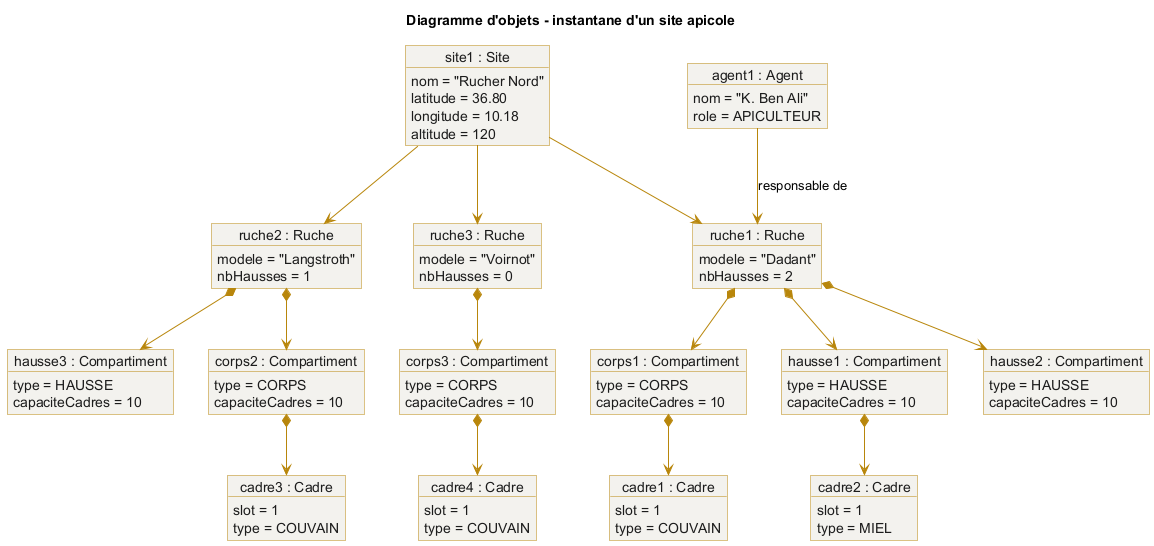
\includegraphics[width=0.7\linewidth]{diagramme_objets}
\caption{Diagramme d'objets, instantané d'un site apicole.}
\label{fig:objets}
\end{figure}

\section{Diagramme d'activité}
Le diagramme d'activité modélise le processus de planification, d'approbation et
de réalisation d'une visite, avec les variantes en ligne et hors-ligne.
\begin{figure}[htbp]
\centering
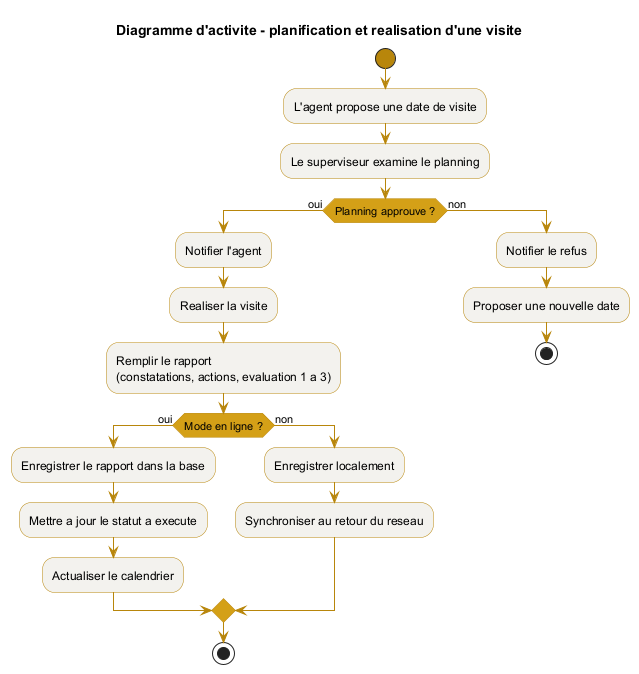
\includegraphics[width=0.7\linewidth]{diagramme_activite}
\caption{Diagramme d'activité du processus de visite.}
\label{fig:activite}
\end{figure}

\section{Diagramme de machine à états}
Le diagramme de machine à états décrit le cycle de vie d'une ruche, de sa
création à sa clôture.
\begin{figure}[htbp]
\centering
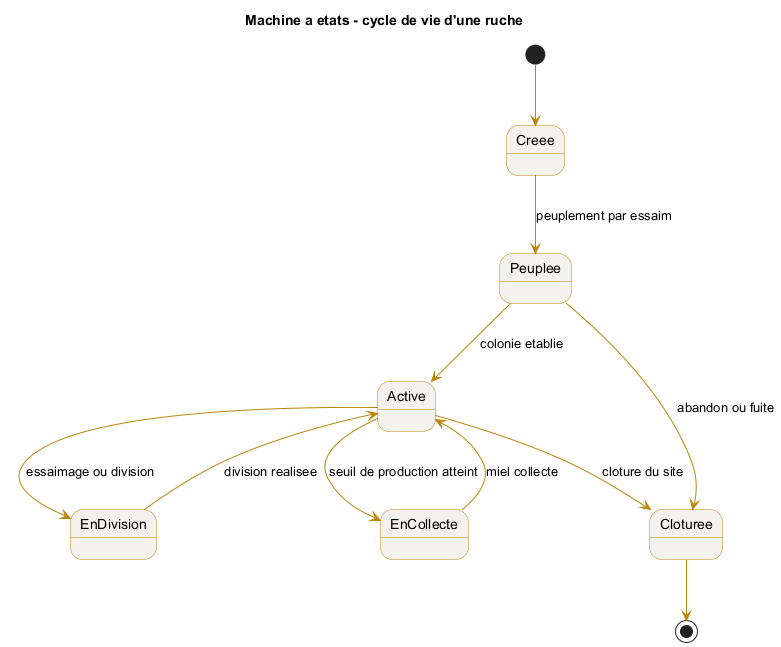
\includegraphics[width=0.85\linewidth]{diagramme_etat}
\caption{Machine à états du cycle de vie d'une ruche.}
\label{fig:etat}
\end{figure}

\section{Diagramme de collaboration}
Le diagramme de collaboration reprend le scénario UC2 sous forme de messages
numérotés échangés entre les objets.
\begin{figure}[htbp]
\centering
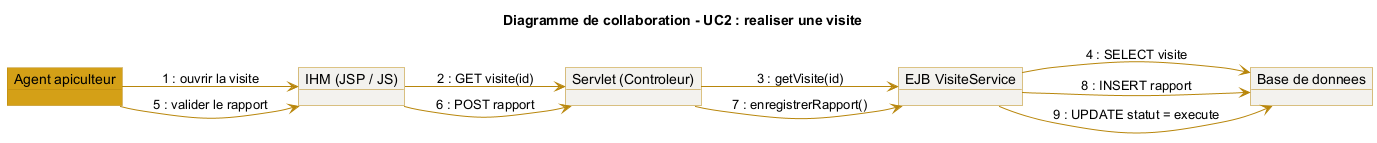
\includegraphics[width=\linewidth]{diagramme_collaboration}
\caption{Diagramme de collaboration du cas d'utilisation UC2.}
\label{fig:collaboration}
\end{figure}

\section{Diagramme de composants}
Le diagramme de composants montre l'organisation des composants applicatifs,
leurs interfaces et leurs dépendances, dont l'interface de service exposant la
quantité de miel.
\begin{figure}[htbp]
\centering
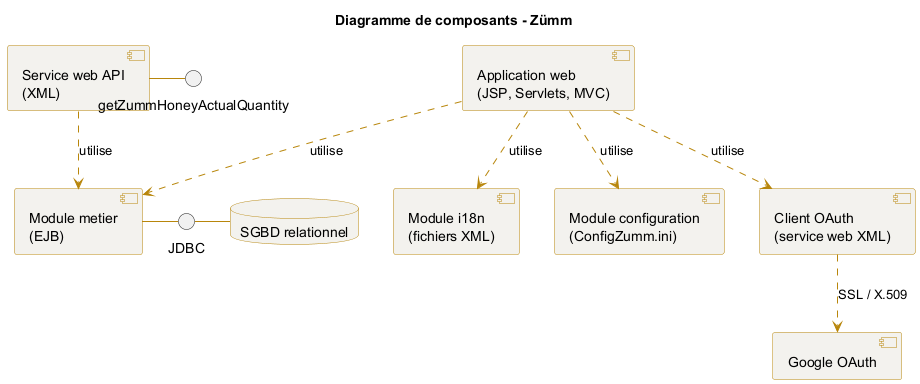
\includegraphics[width=\linewidth]{diagramme_composant}
\caption{Diagramme de composants du système Zümm.}
\label{fig:composant}
\end{figure}

%==============================================================================
\chapter{Contraintes et exigences techniques}
%==============================================================================

\section{Architecture}
Architecture \textbf{scalable, évolutive, flexible, multi-niveaux et faiblement
couplée}, s'appuyant sur \textbf{J2EE} comme infrastructure principale.

\section{Exigences techniques imposées}
\begin{longtable}{>{\bfseries}p{4cm} p{10cm}}
\toprule
\textbf{Exigence} & \textbf{Description} \\
\midrule
\endhead
MVC              & Séparation modèle / vue / contrôleur. \\
Servlet          & Traitement des requêtes côté serveur. \\
JSP              & Front-end de présentation. \\
EJB              & Composants métier. \\
JDBC             & Accès aux données. \\
Internationalisation & Textes de l'IHM externalisés dans un fichier XML, ouverture à la traduction hors-ligne sans limite de langues, FR, EN et AR au minimum en démonstration. \\
Configuration    & Paramétrage par fichier texte \texttt{ConfigZumm.ini}. \\
Sécurité inter-composants & Certificats \textbf{X.509} et protocole \textbf{SSL}. \\
Authentification utilisateur & \textbf{OAuth Google} via un service web XML et son API. \\
API tierce       & Service web XML exposant \texttt{float getZummHoneyActualQuantity(int zummID)} pour récupérer la quantité de miel d'une ruche. \\
Front-end        & JavaScript et frameworks libres, dans le respect de l'ergonomie imposée. \\
\bottomrule
\end{longtable}

\section{Exigences non fonctionnelles}
\begin{itemize}
  \item \textbf{Ergonomie, convivialité et simplicité} d'utilisation, consistance de l'interface et qualité du design infographique (importance capitale).
  \item \textbf{Évolutivité} : ouverture à l'ajout de langues, d'unités et d'indicateurs.
  \item \textbf{Interopérabilité} : services web interrogeables par des applications tierces.
  \item \textbf{Sécurité} : chiffrement des échanges et authentification forte.
  \item \textbf{Qualité de conception} : respect des principes \textbf{SOLID} et recours aux \textbf{design patterns} (patrons de conception) pour garantir un couplage faible et l'évolutivité, comme détaillé en annexe~\ref{chap:solid}.
\end{itemize}

\begin{encadre}
\textbf{Principes de conception retenus :} l'architecture applique les cinq
principes \textbf{SOLID} (responsabilité unique, ouvert/fermé, substitution de
Liskov, ségrégation des interfaces, inversion de dépendance) et un ensemble de
\textbf{design patterns} (Composite, State, Strategy, Observer, Command, Factory
Method, Builder, Adapter, Facade, Singleton, Proxy). Leur application au
système, justifiée « avant / après », est détaillée dans
l'annexe~\ref{chap:solid}.
\end{encadre}

\section{Questions de conception à couvrir}
La conception devra répondre explicitement aux questions suivantes :
\begin{enumerate}
  \item Quels sont les \textbf{inputs} (liste, dictionnaire de données et types) et \textbf{outputs} (liste, dictionnaire, types, formules et requêtes de calcul) du système ?
  \item De quoi se compose la solution ?
  \item Quels sont les utilisateurs types et leurs droits d'accès aux fonctionnalités ?
  \item Comment le système réalise-t-il les opérations utilisateur ?
  \item Comment le système est-il packagé et déployé ?
  \item Comment les éléments interagissent-ils et dans quel ordre / chronologie ?
  \item Pourquoi, comment et où telle technologie a-t-elle été utilisée ?
\end{enumerate}

\section{Justification des choix technologiques}
Le tableau suivant répond au pourquoi, au comment et au où de chaque technologie
imposée. Les \textbf{implémentations concrètes} de ce socle (serveur
d'applications, SGBD, bibliothèques front-end, style de service web) et le
\textbf{comparatif justifié} des alternatives évaluées sont détaillés à
l'annexe~\ref{chap:technologies}.
\begin{longtable}{>{\bfseries}p{2.6cm} p{6cm} p{5.4cm}}
\toprule
\textbf{Technologie} & \textbf{Pourquoi} & \textbf{Où} \\
\midrule
\endhead
MVC & Séparer les responsabilités et faciliter la maintenance & Organisation générale de l'application \\
Servlet & Traiter les requêtes et orchestrer les traitements & Couche de contrôle \\
JSP & Produire les pages dynamiques & Couche de présentation \\
EJB & Encapsuler la logique métier et la rendre réutilisable & Couche métier \\
JDBC & Accéder à la base relationnelle de façon standard & Couche d'accès aux données \\
XML i18n & Externaliser les textes pour la traduction hors-ligne & Module d'internationalisation \\
ConfigZumm.ini & Paramétrer le système sans recompilation & Module de configuration \\
OAuth Google & Authentifier les utilisateurs sans gérer les mots de passe & Accès au système \\
Service web API XML & Exposer les données aux applications tierces & Interface d'interopérabilité \\
X.509 et SSL & Chiffrer et authentifier les échanges & Communications inter-composants \\
JavaScript & Enrichir l'ergonomie du front-end & Couche de présentation \\
\bottomrule
\end{longtable}

\section{Packaging et déploiement}
\begin{itemize}
  \item \textbf{Packaging} : l'application est empaquetée sous forme d'archive Java d'entreprise (WAR pour la partie web, EAR si les EJB sont regroupés), incluant les fichiers XML d'internationalisation et le fichier \texttt{ConfigZumm.ini}.
  \item \textbf{Serveur} : déploiement sur un serveur d'applications J2EE fournissant conteneur de servlets et conteneur d'EJB.
  \item \textbf{Base de données} : SGBD relationnel accédé via JDBC.
  \item \textbf{Sécurité} : installation des certificats X.509 et activation de SSL pour les échanges, configuration de l'accès OAuth Google.
  \item \textbf{Configuration} : les seuils, unités et modules actifs sont ajustés dans \texttt{ConfigZumm.ini} sans redéploiement.
\end{itemize}
La répartition physique est illustrée par le diagramme de déploiement (figure \ref{fig:deploiement}).

%==============================================================================
\chapter{Enveloppe budgétaire et ressources}
%==============================================================================

\section{Cadre}
Le projet s'inscrit dans un cadre \textbf{académique (mini-projet)}. L'enveloppe
budgétaire se traduit donc principalement en \textbf{ressources humaines,
logicielles et matérielles} mobilisées, sans coût financier direct.

\section{Ressources mobilisées}
\begin{longtable}{>{\bfseries}p{4cm} p{10cm}}
\toprule
\textbf{Ressource} & \textbf{Détail} \\
\midrule
\endhead
Humaines   & Équipe projet étudiante (conception, développement, tests, documentation). \\
Logicielles & Serveur d'applications J2EE, SGBD relationnel, IDE, outils UML, chaîne de compilation. \\
Matérielles & Postes de développement, capteurs simulés pour le volet indicateurs. \\
Externes   & Compte OAuth Google, certificats X.509 (auto-signés en démonstration). \\
\bottomrule
\end{longtable}

\begin{encadre}
\textbf{Contrainte académique majeure :} tout usage de générateurs de code
(ChatGPT, DeepSeek et dérivés) est proscrit et sera considéré comme une fraude
à l'épreuve d'examen.
\end{encadre}

%==============================================================================
\chapter{Délais et livrables}
%==============================================================================

\section{Livrables attendus}
\begin{itemize}
  \item Application fonctionnelle (code source J2EE + front-end).
  \item Plan de tests et résultats d'exécution.
  \item Dossier de conception (diagrammes UML).
  \item Rapport de projet, poster et présentation orale.
\end{itemize}

\section{Grille d'évaluation (barème)}
\begin{longtable}{p{9.5cm} C{2.5cm}}
\toprule
\textbf{Critère} & \textbf{Points} \\
\midrule
\endhead
Ergonomie & 4 \\
Fonctionnalités testées (plan de tests + exécution) & 4 \\
\textbf{Technologies} & \textbf{4} \\
\quad MVC & 0,5 \\
\quad Servlet & 0,5 \\
\quad JSP front-end & 0,25 \\
\quad Fichier XML et internationalisation & 0,5 \\
\quad Fichier texte de configuration & 0,25 \\
\quad Web service client OAuth & 0,5 \\
\quad Web service API XML & 0,5 \\
\quad JDBC & 0,5 \\
\quad X.509 / SSL & 0,25 \\
\quad EJB & 0,25 \\
\textbf{Conception} (UC, classes, objets, séquence, activité, état, & \\
\quad interaction/collaboration, package, composant, déploiement) & 4 \\
\textbf{Documentation} & \textbf{4} \\
\quad Rapport (structure, consistance, format) & 2 \\
\quad Poster & 1 \\
\quad Présentation & 1 \\
\midrule
\textbf{Total} & \textbf{20} \\
\bottomrule
\end{longtable}

\section{Diagrammes UML à produire}
Diagrammes de : cas d'utilisation, classes, objets, séquence, activité, machine
à états, interaction / collaboration, package, composant et déploiement. Le
contenu attendu de chacun est détaillé au chapitre \ref{chap:conception} portant
sur la conception.

\section{Planning prévisionnel}
Le planning est exprimé en semaines relatives, avec les livrables intermédiaires
associés à chaque phase.
\begin{longtable}{>{\bfseries}p{4.5cm} C{2.2cm} p{6.5cm}}
\toprule
\textbf{Phase} & \textbf{Semaines} & \textbf{Livrable} \\
\midrule
\endhead
Analyse et cahier des charges & S1 à S2 & Cahier des charges validé \\
Conception (UML) & S3 à S4 & Dossier de conception \\
Développement du noyau CRUD & S5 à S7 & Modèle et gestion des entités \\
Tableaux de bord et alertes & S8 à S9 & Calendrier, alertes et synthèses \\
Services web, sécurité, i18n & S10 à S11 & OAuth, API, X.509 et SSL, XML \\
Tests et validation & S12 & Plan de tests exécuté \\
Documentation et présentation & S13 & Rapport, poster et soutenance \\
\bottomrule
\end{longtable}

%==============================================================================
\chapter{Plan de tests et validation}
%==============================================================================
La stratégie de test couvre les fonctions métier, les contraintes de gestion et
les exigences techniques. Chaque cas de test précise la fonction visée, les
préconditions, les étapes et le résultat attendu.

\section{Cas de tests}
\begin{longtable}{>{\bfseries}p{1.4cm} p{3.6cm} p{4.2cm} p{4.4cm}}
\toprule
\textbf{ID} & \textbf{Fonction} & \textbf{Étapes} & \textbf{Résultat attendu} \\
\midrule
\endhead
TC01 & CRUD ruche & Créer, lire, modifier, supprimer une ruche & Opérations conformes et persistées \\
TC02 & Contrainte cadres & Ajouter un 11e cadre à un corps & Refus, maximum de 10 cadres \\
TC03 & Contrainte hausses & Ajouter une 6e hausse & Refus, maximum de 5 hausses \\
TC04 & Contrainte socle & Retirer le dernier cadre du corps & Refus, au moins 1 cadre \\
TC05 & Planning de visite & Proposer puis approuver une visite & Statut approuvé enregistré \\
TC06 & Rapport de visite & Remplir tous les champs et enregistrer & Rapport persisté, case exécutée \\
TC07 & Alerte production & Dépasser le seuil de production & Alerte de collecte affichée \\
TC08 & Alerte baisse & Simuler une chute d'effectif & Alerte d'inspection affichée \\
TC09 & Calcul ROI & Saisir coûts et production & ROI calculé correctement \\
TC10 & API miel & Appeler getZummHoneyActualQuantity & Quantité correcte retournée \\
TC11 & Internationalisation & Basculer FR, EN puis AR & Textes traduits via le fichier XML \\
TC12 & Configuration & Modifier un seuil dans ConfigZumm.ini & Nouveau seuil pris en compte \\
TC13 & Authentification & Se connecter par OAuth Google & Accès autorisé \\
TC14 & Sécurité & Vérifier SSL et certificat X.509 & Échanges chiffrés et validés \\
TC15 & Export & Exporter les enregistrements & Fichiers CSV et TXT générés \\
TC16 & Mode hors-ligne & Saisir sans réseau puis reconnecter & Synchronisation réussie \\
\bottomrule
\end{longtable}

\section{Matrice de traçabilité}
La matrice relie chaque exigence à son cas d'utilisation, aux classes et tables
qui la portent, à l'écran (maquette) concerné et aux cas de test qui la valident.
Elle assure la traçabilité de bout en bout, du besoin jusqu'à la vérification.
{\small
\begin{longtable}{>{\bfseries}p{3.4cm} C{1.3cm} p{3.3cm} p{2.5cm} p{2.6cm}}
\toprule
\textbf{Exigence} & \textbf{UC} & \textbf{Classes / Tables} & \textbf{Écran} & \textbf{Tests} \\
\midrule
\endhead
Gestion des entités et contraintes & --- & Ruche, Compartiment, Cadre & Fiche ruche (fig.~\ref{fig:wf-ruche}) & TC01--TC04 \\
Planification et approbation & UC1 & Planning, Agent & Calendrier (fig.~\ref{fig:wf-calendrier}) & TC05 \\
Réalisation et rapport de visite & UC2 & Visite, Photo & Rapport (fig.~\ref{fig:wf-rapport}) & TC06 \\
Tableau de bord production & UC3 & Recolte, Mesure, Seuil & TB prod. (fig.~\ref{fig:wf-production}) & TC07, TC09 \\
Alerte sanitaire / baisse & UC4 & Mesure, Seuil & Calendrier & TC08 \\
Service web API (miel) & UC5 & Ruche, Recolte & --- & TC10 \\
Internationalisation & --- & (i18n XML) & Tous & TC11 \\
Configuration par seuils & --- & Seuil & TB prod. & TC12 \\
Authentification OAuth & --- & Agent & Connexion (fig.~\ref{fig:seq-oauth}) & TC13 \\
Sécurité des échanges & --- & (SSL / X.509) & --- & TC14 \\
Portabilité et export & --- & (export CSV/TXT) & Tous & TC15 \\
Mode hors-ligne & UC2 & Visite (file locale) & Rapport & TC16 \\
\bottomrule
\end{longtable}}

%==============================================================================
\chapter{Référentiel métier et bonnes pratiques apicoles}
%==============================================================================
Ce chapitre précise les connaissances métier qui fondent les règles de gestion,
les seuils paramétrables et les indicateurs du système. Il constitue la base
fonctionnelle sur laquelle reposent les tableaux de bord et les alertes.

\section{Facteurs de production du miel}
La production d'une colonie dépend directement de la météo, de la disponibilité
du pollen et du flux de nectar. Lorsque le flux de nectar est élevé, la reine
pond davantage, la population culmine et le rendement atteint son maximum. En
période de pénurie alimentaire, la ponte et la population diminuent. Le système
doit donc corréler la production mesurée aux périodes et aux saisons, ce qui
justifie le filtrage par mois, semaine, saison et année des tableaux de bord.

\section{Emplacement et configuration d'un site}
Le choix de l'emplacement d'un site conditionne la productivité. Les valeurs de
référence suivantes peuvent alimenter les champs et les contrôles de saisie du
module de gestion des sites.
\begin{longtable}{>{\bfseries}p{5.5cm} p{8.5cm}}
\toprule
\textbf{Critère} & \textbf{Valeur de référence} \\
\midrule
\endhead
Proximité des ressources & Sources de nectar et de pollen à environ 1 km. \\
Accès à l'eau & Eau potable accessible, plusieurs litres consommés par jour et par colonie. \\
Éloignement des habitations & 100 m en zone forestière, 200 m en zone arbustive, 300 m en zone ouverte. \\
Éloignement des cultures traitées & Au moins 3 à 4 km des cultures conventionnelles utilisant des pesticides. \\
Surélévation et inclinaison & Ruches surélevées à environ 1,5 m du sol et légèrement inclinées pour évacuer l'humidité. \\
Protection & Abri contre le soleil intense, le vent et les inondations. \\
\bottomrule
\end{longtable}

\begin{figure}[htbp]
\centering
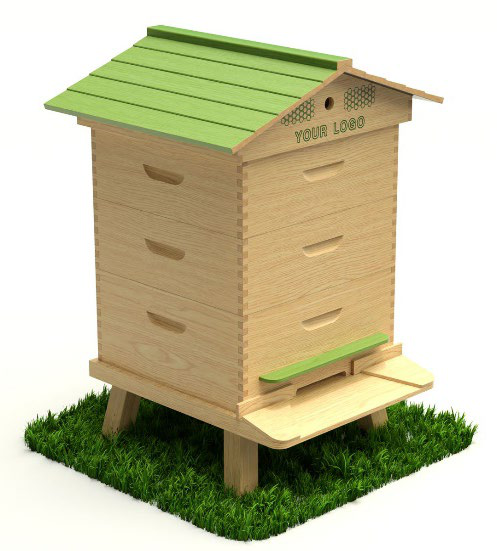
\includegraphics[width=0.48\linewidth]{hive-003}
\caption{Exemple de ruche installée sur un site : surélévation sur pieds et planche d'envol.}
\label{fig:ruche-installee}
\end{figure}

\section{Types de ruches et rendement de référence}
\begin{longtable}{>{\bfseries}p{5.5cm} p{8.5cm}}
\toprule
\textbf{Type de ruche} & \textbf{Caractéristiques et rendement} \\
\midrule
\endhead
Ruche traditionnelle à rayons fixes & 6 à 10 kg de miel en rayons par saison, non recommandée en apiculture biologique. \\
Ruche à barrettes supérieures & Largeur standard de 32 à 35 cm, inspection indépendante des rayons. \\
Ruche à cadres (Langstroth, Est-Africaine) & Rayons à miel réutilisables plusieurs saisons après récolte. \\
\bottomrule
\end{longtable}
Ces ordres de grandeur servent de base au paramétrage des seuils de production
et à l'estimation du retour sur investissement par ruche.

\section{Classification des modèles de ruches}
On distingue deux grandes familles de ruches, dont la modélisation doit rester
ouverte pour couvrir les usages locaux et internationaux.
\begin{longtable}{>{\bfseries}p{4.5cm} p{9.5cm}}
\toprule
\textbf{Famille} & \textbf{Modèles représentatifs} \\
\midrule
\endhead
Ruches à cadres (verticales) & Dadant, Langstroth, Voirnot, Layens, Aumônière, Nationale (GB), WBC, Tonelli. \\
Ruches traditionnelles sans cadres & Warré, Kényane TBH, Tanzanienne TBH, tronc, paille. \\
Autres modèles régionaux & Lucitana, Oksman, Smith, CDB, Duvauchelle, Jarry, Congres, Zanders, modèles slovènes. \\
\bottomrule
\end{longtable}
En France, les modèles les plus courants sont les ruches Dadant, Langstroth et
Voirnot. Toutes les ruches à cadres partagent une composition commune, avec des
dimensions précises au millimètre près, ce qui conforte le modèle de données
retenu.
\begin{encadre}
\textbf{Ancrage du modèle :} le modèle de référence du projet est la ruche
Dadant, dont le corps accueille jusqu'à 10 cadres. Cette valeur fonde la
capacité maximale de 10 cadres par corps ou par hausse retenue dans les règles
de gestion. Le système reste toutefois paramétrable pour supporter d'autres
modèles.
\end{encadre}

\subsection{Composition commune d'une ruche à cadres}
\begin{longtable}{>{\bfseries}p{4cm} p{10cm}}
\toprule
\textbf{Élément} & \textbf{Rôle} \\
\midrule
\endhead
Plancher / planche d'envol & Base de la ruche et zone d'atterrissage des abeilles. \\
Corps (socle) & Compartiment principal du couvain, contient les cadres de base. \\
Hausse & Étage d'extension destiné à la récolte du miel. \\
Cadre & Support amovible des rayons de cire, installé sur un slot identifié. \\
Grille à reine & Sépare le corps des hausses et cantonne la reine dans le corps. \\
Couvre-cadre et toit & Ferment et protègent la ruche des intempéries. \\
Nourrisseur & Permet le ravitaillement en nourriture de la colonie. \\
\bottomrule
\end{longtable}

\begin{figure}[htbp]
\centering
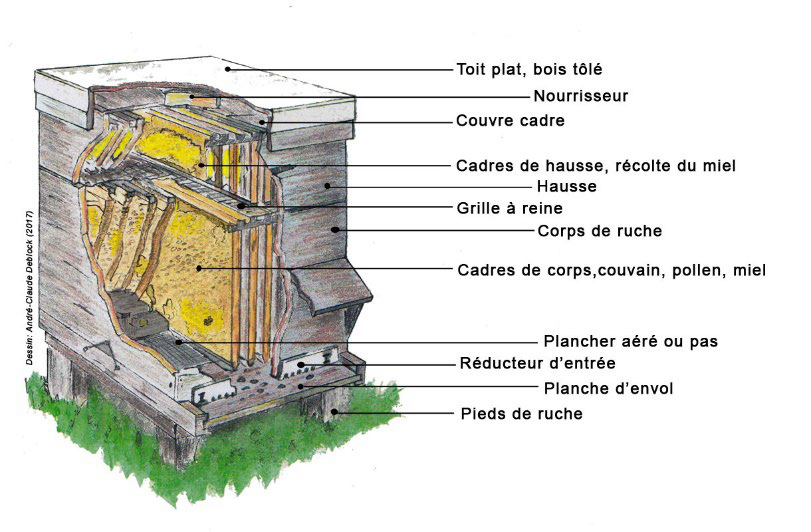
\includegraphics[width=0.85\linewidth]{hive-001}
\caption{Coupe d'une ruche à cadres et rôle de chaque élément (toit, nourrisseur, couvre-cadre, hausse, grille à reine, corps, plancher).}
\label{fig:coupe-ruche}
\end{figure}

\section{Protocole d'inspection des colonies}
Les inspections sont réalisées de préférence les jours ensoleillés et portent
sur des points de contrôle précis qui structurent le rapport de visite.
\begin{itemize}
  \item développement du couvain (oeufs, larves, cellules operculées)
  \item remplissage des alvéoles en miel et en pollen
  \item présence de parasites ou de maladies
  \item récolte de nectar, de pollen et de propolis
\end{itemize}
\begin{encadre}
\textbf{Contrainte opérationnelle :} une visite ne doit pas dépasser 45 minutes.
Au-delà, l'agitation de la colonie augmente et se propage aux ruches voisines.
Le champ \emph{durée} du rapport de visite peut être contrôlé par rapport à
cette limite de référence.
\end{encadre}

\section{Essaimage et division des colonies}
Un essaimage imminent se signale par la présence de cellules royales sur les
bords des rayons. Quelques jours avant l'émergence d'une nouvelle reine, la
vieille reine quitte la colonie avec la moitié des ouvrières. Le système doit
donc permettre d'anticiper la division. Trois méthodes de référence sont
prévues comme motifs d'intervention.
\begin{longtable}{>{\bfseries}p{4.5cm} p{9.5cm}}
\toprule
\textbf{Méthode} & \textbf{Principe} \\
\midrule
\endhead
Formation de nucléus & Retirer 1 à 2 rayons de couvain avec abeilles vers une ruche neuve. \\
Nucléus de reine & Transférer la reine avec un rayon sans cellules royales. \\
Essaimage artificiel & Déplacer la ruche mère et placer une nouvelle ruche à l'ancien emplacement avec 2 à 3 rayons de jeune couvain. \\
\bottomrule
\end{longtable}

\section{Indicateurs de bien-être et causes de baisse}
Une colonie saine présente un nid à couvain bien développé aux différents
stades, des alvéoles remplies de ressources, une activité de butinage visible
et l'absence de parasites ou de maladies. Ces critères alimentent l'évaluation
qualitative de l'état de santé et le niveau de productivité noté de 1 à 3 dans
le rapport de visite.

La fuite ou l'abandon d'une ruche résulte de perturbations excessives ou de
conditions inadéquates (manque de nourriture ou d'eau, températures extrêmes).
Laisser une réserve de miel à la colonie lors de la récolte réduit ce risque.
Ces phénomènes justifient les alertes de chute soudaine d'effectif ou de
production et les seuils paramétrables associés.

\section{Incidence sur les seuils paramétrables}
\begin{longtable}{>{\bfseries}p{4.5cm} p{9.5cm}}
\toprule
\textbf{Paramètre système} & \textbf{Ancrage métier} \\
\midrule
\endhead
Seuil de collecte de miel & Rendement de référence par type de ruche et par saison. \\
Seuil d'alerte de baisse & Chute anormale liée à une fuite, une maladie ou une pénurie alimentaire. \\
Durée maximale de visite & Limite de 45 minutes par inspection. \\
Distances de sécurité du site & 100, 200 ou 300 m selon la zone, 3 à 4 km des cultures traitées. \\
Périodes d'analyse & Corrélation production et saison (flux de nectar). \\
\bottomrule
\end{longtable}

%==============================================================================
\appendix
\chapter{Annexe : Structure physique d'une ruche}
%==============================================================================
Pour mémoire, une ruche à cadres amovibles se compose, de bas en haut, des
éléments suivants : plancher / planche d'envol, corps (socle) contenant les
cadres de couvain, grille à reine, une ou plusieurs hausses contenant les cadres
de récolte du miel, couvre-cadre et toit. Cette structure justifie les règles de
composition (corps obligatoire, jusqu'à 5 hausses, 1 à 10 cadres par élément)
retenues dans le modèle métier.

\begin{figure}[htbp]
\centering
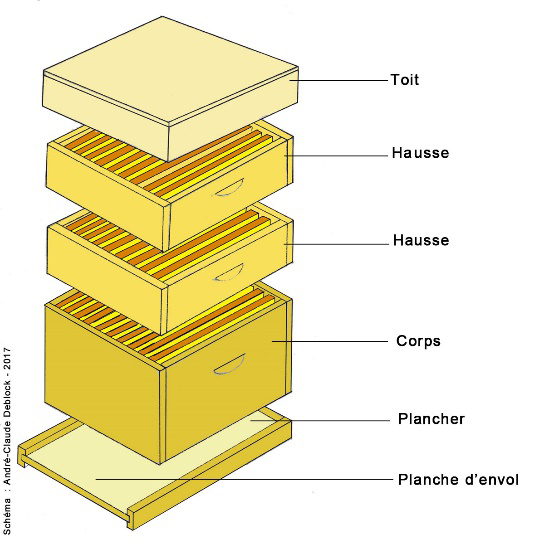
\includegraphics[width=0.55\linewidth]{hive-000}
\caption{Vue éclatée d'une ruche à cadres : toit, hausses, corps, plancher et planche d'envol.}
\label{fig:eclate-ruche}
\end{figure}

%==============================================================================
\chapter{Glossaire}
%==============================================================================
\begin{longtable}{>{\bfseries}p{4cm} p{10cm}}
\toprule
\textbf{Terme} & \textbf{Définition} \\
\midrule
\endhead
Socle ou corps & Compartiment de base de la ruche contenant les cadres de couvain. \\
Hausse & Étage d'extension ajouté au corps pour la récolte du miel. \\
Cadre & Support amovible des rayons de cire, installé sur un slot. \\
Slot & Emplacement identifié d'un cadre dans un corps ou une hausse. \\
Essaim & Colonie d'abeilles peuplant une ruche. \\
Essaimage & Départ d'une partie de la colonie avec la reine pour fonder une nouvelle colonie. \\
Nucléus & Petite colonie constituée pour diviser un essaim ou élever une reine. \\
Reine & Unique femelle reproductrice de la colonie. \\
Couvain & Ensemble des oeufs, larves et nymphes de la colonie. \\
Butinage & Activité de collecte du nectar et du pollen par les abeilles. \\
Propolis & Substance résineuse récoltée par les abeilles. \\
Grille à reine & Grille qui cantonne la reine dans le corps et sépare les hausses. \\
Nourrisseur & Dispositif de ravitaillement en nourriture de la colonie. \\
Seuil paramétrable & Valeur de référence configurable déclenchant une alerte. \\
ROI & Retour sur investissement, rapport entre production valorisée et coûts. \\
CRUD & Opérations de création, lecture, mise à jour et suppression. \\
i18n & Internationalisation, adaptation aux langues et aux systèmes d'unités. \\
EJB & Composant métier de l'infrastructure J2EE. \\
Servlet & Composant serveur traitant les requêtes web. \\
JSP & Page serveur produisant l'affichage dynamique. \\
JDBC & Interface d'accès aux bases de données relationnelles. \\
OAuth & Protocole d'autorisation permettant l'authentification déléguée. \\
X.509 et SSL & Certificats et protocole assurant des échanges chiffrés et authentifiés. \\
TLS & Protocole de chiffrement des échanges réseau (couche transport), base de HTTPS. \\
REST / JSON & Style d'API web et format texte d'échange des données (ingestion des mesures). \\
MQTT & Protocole de messagerie léger (publication/abonnement) adapté aux capteurs et aux réseaux contraints. \\
JWT (jeton) & Jeton signé porteur d'identité, émis par le fournisseur OAuth. \\
RBAC & Contrôle d'accès basé sur les rôles, appliqué côté serveur (voir annexe~\ref{chap:complements}). \\
RGPD & Règlement général sur la protection des données ; encadre les données personnelles. \\
Rétention & Durée de conservation d'une donnée avant archivage, anonymisation ou purge. \\
Chiffrement au repos & Chiffrement des données stockées (colonnes sensibles) en base. \\
Pseudonymisation & Dissociation de l'identité d'une personne de ses données, réversible sous contrôle. \\
Idempotence & Propriété d'une opération rejouable sans créer de doublon (ingestion des mesures). \\
Hystérésis & Persistance d'un dépassement sur plusieurs mesures avant de lever une alerte (anti-rebond). \\
\bottomrule
\end{longtable}

%==============================================================================
\chapter{Références et sources}
%==============================================================================
Le présent cahier des charges s'appuie sur les sources suivantes.

\subsection*{Méthode d'élaboration}
\begin{itemize}
  \item Manager-GO, \emph{Élaborer un cahier des charges}.\\ \url{https://www.manager-go.com/gestion-de-projet/dossiers-methodes/elaborer-un-cdc}
\end{itemize}

\subsection*{Principes de conception logicielle}
\begin{itemize}
  \item Alex so yes, \emph{Les principes SOLID}.\\ \url{https://alexsoyes.com/solid/}
  \item Refactoring Guru, \emph{Catalogue des design patterns}.\\ \url{https://refactoring.guru}
\end{itemize}

\subsection*{Référentiel métier apicole}
\begin{itemize}
  \item Organic Africa, \emph{Amélioration de la production de miel}.\\ \url{https://www.organic-africa.net/fr/agriculture-biologique/agriculture-biologique/animaux/apiculture/amelioration-de-la-production-de-miel.html}
  \item Au Bon Miel, \emph{Les ruches}.\\ \url{https://www.aubonmiel.com/les-ruches/}
\end{itemize}

\subsection*{Fonctionnalités des solutions du marché}
\begin{itemize}
  \item HiveTracks, application de gestion apicole.\\ \url{https://www.hivetracks.com/}
  \item Apiary Book, solution de gestion de rucher.\\ \url{https://www.apiarybook.com/}
  \item BeePlus, gestionnaire d'apiculture (App Store).
\end{itemize}

\subsection*{Surveillance connectée (precision beekeeping)}
\begin{itemize}
  \item Arnia, surveillance acoustique et pesée des ruches.\\ \url{https://www.arnia.co/}
  \item BroodMinder, capteurs de température, d'humidité et de poids.\\ \url{https://broodminder.com/}
  \item BeeHero, plateforme IoT et analyse par intelligence artificielle.\\ \url{https://www.beehero.io/}
\end{itemize}

\subsection*{Retours d'expérience et limites des solutions}
\begin{itemize}
  \item Beekeeping Diary, \emph{Best Beekeeping Apps 2026 (comparatif)}.\\ \url{https://beekeeping-diary.eu/blog/en/best-beekeeping-apps-2026/}
  \item HiveBook, \emph{Free HiveTracks Alternatives}.\\ \url{https://hivebook.app/blog/hivetracks-alternatives-free}
  \item Beesource Forums, \emph{Problems with Hive Tracks}.\\ \url{https://www.beesource.com/threads/problems-with-hive-tracks.249656/}
  \item ApiTech World, \emph{Smart Hive Monitoring, a Beekeeper's Reality Check (2026)}.\\ \url{https://apitechworld.com/smart-hive-monitoring-a-beekeepers-reality-check-2026-review/}
\end{itemize}

\input{annexe_technologies}

%==============================================================================
%  ANNEXE - Choix technologique : conformite academique et vision marche
%  Migration J2EE -> Spring Boot (tableau de correspondance + argumentaire)
%  A inserer via %==============================================================================
%  ANNEXE - Choix technologique : conformite academique et vision marche
%  Migration J2EE -> Spring Boot (tableau de correspondance + argumentaire)
%  A inserer via %==============================================================================
%  ANNEXE - Choix technologique : conformite academique et vision marche
%  Migration J2EE -> Spring Boot (tableau de correspondance + argumentaire)
%  A inserer via \input{annexe_migration_springboot} dans cahier_des_charges.tex
%  (utilise la charte "Miel & noir" : miel, mielfonce, encadre, colonne C,
%   longtable, booktabs -- deja definis dans le preambule principal)
%==============================================================================

%==============================================================================
\chapter{Annexe - Choix technologique : academique et vision marche}
\label{chap:migration}
%==============================================================================
Cette annexe repond a la question du \emph{pourquoi} et du \emph{comment} du
langage de developpement. Elle confronte le socle \textbf{J2EE} impose par le
present cahier des charges a l'ecosysteme \textbf{Spring Boot}, devenu le
standard du developpement Java d'entreprise, et documente une trajectoire de
modernisation sans changement de langage.

\section{Positionnement}
Le systeme \textbf{Z\"umm} est implemente en \textbf{J2EE (Java EE)}
conformement aux exigences techniques (chapitre~\ref{chap:conception} et grille
d'evaluation) : MVC, Servlets, JSP, EJB, JDBC, internationalisation
externalisee, services web securises (OAuth, X.509 / SSL) et API interrogeable
par des applications tierces. Ce socle materialise les competences fondamentales
du parcours DSI : maitrise des couches d'un systeme d'information, separation des
responsabilites et interoperabilite.

\begin{encadre}
\textbf{Constat marche :} les briques Java EE historiques (JSP, Servlets
\og nus \fg{} et EJB) sont aujourd'hui considerees comme \emph{heritees}
(\emph{legacy}). Les recrutements sur les nouveaux systemes d'information
privilegient tres majoritairement l'ecosysteme \textbf{Spring Boot}. La presente
annexe conserve le langage \textbf{Java} et demontre, techno par techno,
l'equivalent moderne de chaque exigence.
\end{encadre}

%------------------------------------------------------------------------------
\section{Tableau de correspondance : coeur technique}
%------------------------------------------------------------------------------
Le tableau suivant met en regard chaque technologie imposee (et notee) avec son
equivalent Spring Boot, ainsi que la nature concrete du changement.

\begin{longtable}{>{\bfseries}p{3cm} p{3.4cm} p{7.2cm}}
\toprule
\textbf{J2EE (impose)} & \textbf{Spring Boot} & \textbf{Ce qui change concretement} \\
\midrule
\endhead
MVC (manuel) & Spring MVC (\texttt{@Controller}, \texttt{@RequestMapping}) & Le pattern reste ; le routage devient declaratif par annotations au lieu du \texttt{web.xml}. \\
Servlet (\texttt{HttpServlet}, \texttt{doGet/doPost}) & \texttt{@RestController} / \texttt{@Controller} & Plus de \texttt{extends HttpServlet} : une methode annotee = un endpoint. Le \texttt{DispatcherServlet} orchestre en arriere-plan. \\
JSP (presentation) & Thymeleaf (server-side) ou React / Angular (SPA) & Templating moderne sans scriptlets Java ; pour un effet marche fort, API REST + front decouple. \\
EJB (\texttt{@Stateless}, conteneur EJB) & Spring \texttt{@Service} / \texttt{@Component} & Meme role (logique metier, injection, transactions) sans conteneur EJB lourd ; \texttt{@Transactional} gere les transactions. \\
JDBC (SQL manuel, \texttt{ResultSet}) & Spring Data JPA / Hibernate & Le mapping objet-relationnel remplace le SQL a la main ; \texttt{JpaRepository} genere les CRUD (\texttt{JdbcTemplate} reste disponible). \\
i18n par fichier XML & \texttt{messages\_fr/en/ar.properties} + \texttt{MessageSource} & Meme principe d'externalisation des textes, format \texttt{.properties} standard, toujours FR / EN / AR. \\
\texttt{ConfigZumm.ini} & \texttt{application.yml} + \texttt{@ConfigurationProperties} & Parametrage sans recompilation, injectable par profil ; les seuils et unites deviennent des beans types. \\
OAuth Google (WS XML maison) & Spring Security OAuth2 Client & Login Google en quelques lignes de configuration au lieu d'un client OAuth ecrit a la main, et plus sur. \\
Web service API XML \texttt{getZummHoneyActualQuantity} & API REST JSON (\texttt{@GetMapping}) + OpenAPI / Swagger & JSON au lieu de XML, documentation auto-generee ; XML reste possible via \texttt{produces = APPLICATION\_XML}. \\
X.509 / SSL (manuel) & Spring Boot SSL (\texttt{server.ssl.*}) + Keystore & Activation HTTPS declarative, memes certificats X.509, configuration triviale. \\
JavaScript (front libre) & React / Vue / Angular (ou Thymeleaf + JS) & Front decouple consommant l'API REST, parite web et mobile simplifiee. \\
\bottomrule
\end{longtable}

%------------------------------------------------------------------------------
\section{Tableau de correspondance : infrastructure et deploiement}
%------------------------------------------------------------------------------
\begin{longtable}{>{\bfseries}p{4cm} p{4.5cm} p{5.3cm}}
\toprule
\textbf{J2EE} & \textbf{Spring Boot} & \textbf{Benefice} \\
\midrule
\endhead
Serveur d'applications lourd (WildFly, GlassFish, WebLogic) & Tomcat / Jetty embarque & L'application se lance seule : \texttt{java -jar app.jar}, plus de serveur a installer. \\
Packaging WAR / EAR & JAR executable (fat-jar) & Un seul artefact autonome, ideal pour le cloud et Docker. \\
Deploiement manuel sur conteneur & Docker + \texttt{docker-compose} & Alignement DevOps du marche, integration continue facilitee. \\
SGBD relationnel via JDBC & PostgreSQL / MySQL via JPA + Flyway & Schema versionne, reproductible entre environnements. \\
Gestion des dependances manuelle (Ant) & Maven / Gradle + Spring Boot Starters & Une dependance = un starter (\texttt{-web}, \texttt{-security}, \texttt{-data-jpa}). \\
\bottomrule
\end{longtable}

%------------------------------------------------------------------------------
\section{Correspondance des couches}
%------------------------------------------------------------------------------
La vue en couches faiblement couplees exigee au chapitre~\ref{chap:conception}
(figure~\ref{fig:couches}) est \textbf{integralement preservee} : aucune couche
ne disparait, seule la mise en oeuvre est modernisee.

\begin{figure}[htbp]
\centering
\begin{tikzpicture}[
  j2ee/.style={draw=mielfonce,fill=grisdoux,thick,minimum width=5.4cm,minimum height=8mm,font=\footnotesize,align=center},
  spring/.style={draw=mielfonce,fill=miel!15,thick,minimum width=5.4cm,minimum height=8mm,font=\footnotesize,align=center},
  fl/.style={-{Latex[length=2mm]},mielfonce,thick}
]
% en-tetes
\node[font=\small\bfseries,mielfonce] at (0,5) {J2EE (impose)};
\node[font=\small\bfseries,mielfonce] at (7,5) {Spring Boot (cible)};
% couches J2EE
\node[j2ee] (p1) at (0,4) {Presentation : JSP + JavaScript};
\node[j2ee] (c1) at (0,3) {Controle : Servlets (MVC)};
\node[j2ee] (m1) at (0,2) {Metier : EJB};
\node[j2ee] (d1) at (0,1) {Acces donnees : JDBC};
\node[j2ee] (b1) at (0,0) {Base de donnees relationnelle};
% couches Spring
\node[spring] (p2) at (7,4) {@Controller + Thymeleaf / React};
\node[spring] (c2) at (7,3) {@RestController (Spring MVC)};
\node[spring] (m2) at (7,2) {@Service (Spring Beans)};
\node[spring] (d2) at (7,1) {@Repository (Spring Data JPA)};
\node[spring] (b2) at (7,0) {PostgreSQL / MySQL (inchange)};
% fleches de correspondance
\draw[fl] (p1)--(p2); \draw[fl] (c1)--(c2); \draw[fl] (m1)--(m2);
\draw[fl] (d1)--(d2); \draw[fl] (b1)--(b2);
\end{tikzpicture}
\caption{Correspondance des couches J2EE vers Spring Boot : architecture preservee, mise en oeuvre modernisee.}
\label{fig:migration-couches}
\end{figure}

Les modules transverses suivent la meme logique : i18n XML \textrightarrow{}
\texttt{MessageSource}, \texttt{ConfigZumm.ini} \textrightarrow{}
\texttt{application.yml}, service web XML \textrightarrow{} API REST + OpenAPI.

%------------------------------------------------------------------------------
\section{Argumentaire : conformite academique et vision marche}
%------------------------------------------------------------------------------
\textbf{Z\"umm} repose, conformement au cahier des charges, sur une
architecture \textbf{J2EE multi-niveaux, evolutive et faiblement couplee} : MVC,
Servlets, JSP, EJB, JDBC, internationalisation par fichier externalise, services
web securises (OAuth, X.509 / SSL) et API interrogeable par des applications
tierces. Ce socle a ete retenu et implemente \textbf{tel qu'exige}, car il
constitue le referentiel d'evaluation du projet et materialise les competences
fondamentales du parcours DSI : maitrise des couches d'un systeme d'information,
separation des responsabilites et interoperabilite.

Une analyse \textbf{orientee marche} conduit toutefois a un constat important.
Les briques Java EE historiques (JSP, Servlets \og nus \fg{} et EJB) sont
aujourd'hui considerees comme \emph{heritees}. Les recrutements sur les nouveaux
systemes d'information privilegient tres majoritairement l'ecosysteme
\textbf{Spring Boot}, devenu le standard \emph{de facto} du developpement Java
d'entreprise. Ignorer cette realite reviendrait a livrer une solution
techniquement conforme mais \textbf{decalee des pratiques professionnelles
actuelles}.

Nous avons donc adopte une \textbf{demarche a deux niveaux de lecture}, sans
jamais sortir du langage \textbf{Java}, ce qui garantit la continuite des
competences acquises :
\begin{enumerate}
  \item \textbf{Niveau conformite} : le livrable respecte integralement les
        technologies imposees et la grille d'evaluation. Les diagrammes de
        conception (sequence Agent \textrightarrow{} JSP \textrightarrow{}
        Servlet \textrightarrow{} EJB \textrightarrow{} JDBC, couches,
        deploiement) refletent fidelement cette architecture.
  \item \textbf{Niveau modernisation} : pour chaque technologie imposee, son
        equivalent Spring Boot est demontre (Servlet \textrightarrow{}
        \texttt{@RestController}, EJB \textrightarrow{} \texttt{@Service}, JDBC
        \textrightarrow{} Spring Data JPA, XML i18n \textrightarrow{}
        \texttt{MessageSource}, \texttt{ConfigZumm.ini} \textrightarrow{}
        \texttt{application.yml}, WS XML \textrightarrow{} API REST + OpenAPI,
        X.509 / SSL \textrightarrow{} configuration SSL declarative). Cette
        correspondance prouve que \textbf{l'architecture cible reste identique} :
        seule la mise en oeuvre gagne en concision, en securite et en
        maintenabilite.
\end{enumerate}

Ce choix presente un troisieme avantage, en phase directe avec les debouches du
parcours DSI. Le cahier des charges prevoit un \textbf{volet capteurs et analyse
predictive} (detection d'essaimage, traitement acoustique). Ce module se prete
naturellement a un \textbf{microservice Python} (pandas, scikit-learn) expose au
back-end Java via REST, illustrant concretement le metier d'\textbf{analyste de
donnees} cite au plan d'etudes et l'ouverture d'une \textbf{architecture
faiblement couplee} a l'heterogeneite technologique.

\begin{encadre}
\textbf{Conclusion :} le projet satisfait pleinement les exigences academiques
(J2EE) tout en documentant sa \textbf{trajectoire de modernisation} (Spring Boot
et microservice data). Cette double lecture transforme une contrainte
pedagogique en atout professionnel : elle demontre non seulement la maitrise des
fondamentaux du systeme d'information, mais aussi la capacite a faire evoluer une
architecture vers les standards recherches sur le marche de l'emploi en 2026.
\end{encadre} dans cahier_des_charges.tex
%  (utilise la charte "Miel & noir" : miel, mielfonce, encadre, colonne C,
%   longtable, booktabs -- deja definis dans le preambule principal)
%==============================================================================

%==============================================================================
\chapter{Annexe - Choix technologique : academique et vision marche}
\label{chap:migration}
%==============================================================================
Cette annexe repond a la question du \emph{pourquoi} et du \emph{comment} du
langage de developpement. Elle confronte le socle \textbf{J2EE} impose par le
present cahier des charges a l'ecosysteme \textbf{Spring Boot}, devenu le
standard du developpement Java d'entreprise, et documente une trajectoire de
modernisation sans changement de langage.

\section{Positionnement}
Le systeme \textbf{Z\"umm} est implemente en \textbf{J2EE (Java EE)}
conformement aux exigences techniques (chapitre~\ref{chap:conception} et grille
d'evaluation) : MVC, Servlets, JSP, EJB, JDBC, internationalisation
externalisee, services web securises (OAuth, X.509 / SSL) et API interrogeable
par des applications tierces. Ce socle materialise les competences fondamentales
du parcours DSI : maitrise des couches d'un systeme d'information, separation des
responsabilites et interoperabilite.

\begin{encadre}
\textbf{Constat marche :} les briques Java EE historiques (JSP, Servlets
\og nus \fg{} et EJB) sont aujourd'hui considerees comme \emph{heritees}
(\emph{legacy}). Les recrutements sur les nouveaux systemes d'information
privilegient tres majoritairement l'ecosysteme \textbf{Spring Boot}. La presente
annexe conserve le langage \textbf{Java} et demontre, techno par techno,
l'equivalent moderne de chaque exigence.
\end{encadre}

%------------------------------------------------------------------------------
\section{Tableau de correspondance : coeur technique}
%------------------------------------------------------------------------------
Le tableau suivant met en regard chaque technologie imposee (et notee) avec son
equivalent Spring Boot, ainsi que la nature concrete du changement.

\begin{longtable}{>{\bfseries}p{3cm} p{3.4cm} p{7.2cm}}
\toprule
\textbf{J2EE (impose)} & \textbf{Spring Boot} & \textbf{Ce qui change concretement} \\
\midrule
\endhead
MVC (manuel) & Spring MVC (\texttt{@Controller}, \texttt{@RequestMapping}) & Le pattern reste ; le routage devient declaratif par annotations au lieu du \texttt{web.xml}. \\
Servlet (\texttt{HttpServlet}, \texttt{doGet/doPost}) & \texttt{@RestController} / \texttt{@Controller} & Plus de \texttt{extends HttpServlet} : une methode annotee = un endpoint. Le \texttt{DispatcherServlet} orchestre en arriere-plan. \\
JSP (presentation) & Thymeleaf (server-side) ou React / Angular (SPA) & Templating moderne sans scriptlets Java ; pour un effet marche fort, API REST + front decouple. \\
EJB (\texttt{@Stateless}, conteneur EJB) & Spring \texttt{@Service} / \texttt{@Component} & Meme role (logique metier, injection, transactions) sans conteneur EJB lourd ; \texttt{@Transactional} gere les transactions. \\
JDBC (SQL manuel, \texttt{ResultSet}) & Spring Data JPA / Hibernate & Le mapping objet-relationnel remplace le SQL a la main ; \texttt{JpaRepository} genere les CRUD (\texttt{JdbcTemplate} reste disponible). \\
i18n par fichier XML & \texttt{messages\_fr/en/ar.properties} + \texttt{MessageSource} & Meme principe d'externalisation des textes, format \texttt{.properties} standard, toujours FR / EN / AR. \\
\texttt{ConfigZumm.ini} & \texttt{application.yml} + \texttt{@ConfigurationProperties} & Parametrage sans recompilation, injectable par profil ; les seuils et unites deviennent des beans types. \\
OAuth Google (WS XML maison) & Spring Security OAuth2 Client & Login Google en quelques lignes de configuration au lieu d'un client OAuth ecrit a la main, et plus sur. \\
Web service API XML \texttt{getZummHoneyActualQuantity} & API REST JSON (\texttt{@GetMapping}) + OpenAPI / Swagger & JSON au lieu de XML, documentation auto-generee ; XML reste possible via \texttt{produces = APPLICATION\_XML}. \\
X.509 / SSL (manuel) & Spring Boot SSL (\texttt{server.ssl.*}) + Keystore & Activation HTTPS declarative, memes certificats X.509, configuration triviale. \\
JavaScript (front libre) & React / Vue / Angular (ou Thymeleaf + JS) & Front decouple consommant l'API REST, parite web et mobile simplifiee. \\
\bottomrule
\end{longtable}

%------------------------------------------------------------------------------
\section{Tableau de correspondance : infrastructure et deploiement}
%------------------------------------------------------------------------------
\begin{longtable}{>{\bfseries}p{4cm} p{4.5cm} p{5.3cm}}
\toprule
\textbf{J2EE} & \textbf{Spring Boot} & \textbf{Benefice} \\
\midrule
\endhead
Serveur d'applications lourd (WildFly, GlassFish, WebLogic) & Tomcat / Jetty embarque & L'application se lance seule : \texttt{java -jar app.jar}, plus de serveur a installer. \\
Packaging WAR / EAR & JAR executable (fat-jar) & Un seul artefact autonome, ideal pour le cloud et Docker. \\
Deploiement manuel sur conteneur & Docker + \texttt{docker-compose} & Alignement DevOps du marche, integration continue facilitee. \\
SGBD relationnel via JDBC & PostgreSQL / MySQL via JPA + Flyway & Schema versionne, reproductible entre environnements. \\
Gestion des dependances manuelle (Ant) & Maven / Gradle + Spring Boot Starters & Une dependance = un starter (\texttt{-web}, \texttt{-security}, \texttt{-data-jpa}). \\
\bottomrule
\end{longtable}

%------------------------------------------------------------------------------
\section{Correspondance des couches}
%------------------------------------------------------------------------------
La vue en couches faiblement couplees exigee au chapitre~\ref{chap:conception}
(figure~\ref{fig:couches}) est \textbf{integralement preservee} : aucune couche
ne disparait, seule la mise en oeuvre est modernisee.

\begin{figure}[htbp]
\centering
\begin{tikzpicture}[
  j2ee/.style={draw=mielfonce,fill=grisdoux,thick,minimum width=5.4cm,minimum height=8mm,font=\footnotesize,align=center},
  spring/.style={draw=mielfonce,fill=miel!15,thick,minimum width=5.4cm,minimum height=8mm,font=\footnotesize,align=center},
  fl/.style={-{Latex[length=2mm]},mielfonce,thick}
]
% en-tetes
\node[font=\small\bfseries,mielfonce] at (0,5) {J2EE (impose)};
\node[font=\small\bfseries,mielfonce] at (7,5) {Spring Boot (cible)};
% couches J2EE
\node[j2ee] (p1) at (0,4) {Presentation : JSP + JavaScript};
\node[j2ee] (c1) at (0,3) {Controle : Servlets (MVC)};
\node[j2ee] (m1) at (0,2) {Metier : EJB};
\node[j2ee] (d1) at (0,1) {Acces donnees : JDBC};
\node[j2ee] (b1) at (0,0) {Base de donnees relationnelle};
% couches Spring
\node[spring] (p2) at (7,4) {@Controller + Thymeleaf / React};
\node[spring] (c2) at (7,3) {@RestController (Spring MVC)};
\node[spring] (m2) at (7,2) {@Service (Spring Beans)};
\node[spring] (d2) at (7,1) {@Repository (Spring Data JPA)};
\node[spring] (b2) at (7,0) {PostgreSQL / MySQL (inchange)};
% fleches de correspondance
\draw[fl] (p1)--(p2); \draw[fl] (c1)--(c2); \draw[fl] (m1)--(m2);
\draw[fl] (d1)--(d2); \draw[fl] (b1)--(b2);
\end{tikzpicture}
\caption{Correspondance des couches J2EE vers Spring Boot : architecture preservee, mise en oeuvre modernisee.}
\label{fig:migration-couches}
\end{figure}

Les modules transverses suivent la meme logique : i18n XML \textrightarrow{}
\texttt{MessageSource}, \texttt{ConfigZumm.ini} \textrightarrow{}
\texttt{application.yml}, service web XML \textrightarrow{} API REST + OpenAPI.

%------------------------------------------------------------------------------
\section{Argumentaire : conformite academique et vision marche}
%------------------------------------------------------------------------------
\textbf{Z\"umm} repose, conformement au cahier des charges, sur une
architecture \textbf{J2EE multi-niveaux, evolutive et faiblement couplee} : MVC,
Servlets, JSP, EJB, JDBC, internationalisation par fichier externalise, services
web securises (OAuth, X.509 / SSL) et API interrogeable par des applications
tierces. Ce socle a ete retenu et implemente \textbf{tel qu'exige}, car il
constitue le referentiel d'evaluation du projet et materialise les competences
fondamentales du parcours DSI : maitrise des couches d'un systeme d'information,
separation des responsabilites et interoperabilite.

Une analyse \textbf{orientee marche} conduit toutefois a un constat important.
Les briques Java EE historiques (JSP, Servlets \og nus \fg{} et EJB) sont
aujourd'hui considerees comme \emph{heritees}. Les recrutements sur les nouveaux
systemes d'information privilegient tres majoritairement l'ecosysteme
\textbf{Spring Boot}, devenu le standard \emph{de facto} du developpement Java
d'entreprise. Ignorer cette realite reviendrait a livrer une solution
techniquement conforme mais \textbf{decalee des pratiques professionnelles
actuelles}.

Nous avons donc adopte une \textbf{demarche a deux niveaux de lecture}, sans
jamais sortir du langage \textbf{Java}, ce qui garantit la continuite des
competences acquises :
\begin{enumerate}
  \item \textbf{Niveau conformite} : le livrable respecte integralement les
        technologies imposees et la grille d'evaluation. Les diagrammes de
        conception (sequence Agent \textrightarrow{} JSP \textrightarrow{}
        Servlet \textrightarrow{} EJB \textrightarrow{} JDBC, couches,
        deploiement) refletent fidelement cette architecture.
  \item \textbf{Niveau modernisation} : pour chaque technologie imposee, son
        equivalent Spring Boot est demontre (Servlet \textrightarrow{}
        \texttt{@RestController}, EJB \textrightarrow{} \texttt{@Service}, JDBC
        \textrightarrow{} Spring Data JPA, XML i18n \textrightarrow{}
        \texttt{MessageSource}, \texttt{ConfigZumm.ini} \textrightarrow{}
        \texttt{application.yml}, WS XML \textrightarrow{} API REST + OpenAPI,
        X.509 / SSL \textrightarrow{} configuration SSL declarative). Cette
        correspondance prouve que \textbf{l'architecture cible reste identique} :
        seule la mise en oeuvre gagne en concision, en securite et en
        maintenabilite.
\end{enumerate}

Ce choix presente un troisieme avantage, en phase directe avec les debouches du
parcours DSI. Le cahier des charges prevoit un \textbf{volet capteurs et analyse
predictive} (detection d'essaimage, traitement acoustique). Ce module se prete
naturellement a un \textbf{microservice Python} (pandas, scikit-learn) expose au
back-end Java via REST, illustrant concretement le metier d'\textbf{analyste de
donnees} cite au plan d'etudes et l'ouverture d'une \textbf{architecture
faiblement couplee} a l'heterogeneite technologique.

\begin{encadre}
\textbf{Conclusion :} le projet satisfait pleinement les exigences academiques
(J2EE) tout en documentant sa \textbf{trajectoire de modernisation} (Spring Boot
et microservice data). Cette double lecture transforme une contrainte
pedagogique en atout professionnel : elle demontre non seulement la maitrise des
fondamentaux du systeme d'information, mais aussi la capacite a faire evoluer une
architecture vers les standards recherches sur le marche de l'emploi en 2026.
\end{encadre} dans cahier_des_charges.tex
%  (utilise la charte "Miel & noir" : miel, mielfonce, encadre, colonne C,
%   longtable, booktabs -- deja definis dans le preambule principal)
%==============================================================================

%==============================================================================
\chapter{Annexe - Choix technologique : academique et vision marche}
\label{chap:migration}
%==============================================================================
Cette annexe repond a la question du \emph{pourquoi} et du \emph{comment} du
langage de developpement. Elle confronte le socle \textbf{J2EE} impose par le
present cahier des charges a l'ecosysteme \textbf{Spring Boot}, devenu le
standard du developpement Java d'entreprise, et documente une trajectoire de
modernisation sans changement de langage.

\section{Positionnement}
Le systeme \textbf{Z\"umm} est implemente en \textbf{J2EE (Java EE)}
conformement aux exigences techniques (chapitre~\ref{chap:conception} et grille
d'evaluation) : MVC, Servlets, JSP, EJB, JDBC, internationalisation
externalisee, services web securises (OAuth, X.509 / SSL) et API interrogeable
par des applications tierces. Ce socle materialise les competences fondamentales
du parcours DSI : maitrise des couches d'un systeme d'information, separation des
responsabilites et interoperabilite.

\begin{encadre}
\textbf{Constat marche :} les briques Java EE historiques (JSP, Servlets
\og nus \fg{} et EJB) sont aujourd'hui considerees comme \emph{heritees}
(\emph{legacy}). Les recrutements sur les nouveaux systemes d'information
privilegient tres majoritairement l'ecosysteme \textbf{Spring Boot}. La presente
annexe conserve le langage \textbf{Java} et demontre, techno par techno,
l'equivalent moderne de chaque exigence.
\end{encadre}

%------------------------------------------------------------------------------
\section{Tableau de correspondance : coeur technique}
%------------------------------------------------------------------------------
Le tableau suivant met en regard chaque technologie imposee (et notee) avec son
equivalent Spring Boot, ainsi que la nature concrete du changement.

\begin{longtable}{>{\bfseries}p{3cm} p{3.4cm} p{7.2cm}}
\toprule
\textbf{J2EE (impose)} & \textbf{Spring Boot} & \textbf{Ce qui change concretement} \\
\midrule
\endhead
MVC (manuel) & Spring MVC (\texttt{@Controller}, \texttt{@RequestMapping}) & Le pattern reste ; le routage devient declaratif par annotations au lieu du \texttt{web.xml}. \\
Servlet (\texttt{HttpServlet}, \texttt{doGet/doPost}) & \texttt{@RestController} / \texttt{@Controller} & Plus de \texttt{extends HttpServlet} : une methode annotee = un endpoint. Le \texttt{DispatcherServlet} orchestre en arriere-plan. \\
JSP (presentation) & Thymeleaf (server-side) ou React / Angular (SPA) & Templating moderne sans scriptlets Java ; pour un effet marche fort, API REST + front decouple. \\
EJB (\texttt{@Stateless}, conteneur EJB) & Spring \texttt{@Service} / \texttt{@Component} & Meme role (logique metier, injection, transactions) sans conteneur EJB lourd ; \texttt{@Transactional} gere les transactions. \\
JDBC (SQL manuel, \texttt{ResultSet}) & Spring Data JPA / Hibernate & Le mapping objet-relationnel remplace le SQL a la main ; \texttt{JpaRepository} genere les CRUD (\texttt{JdbcTemplate} reste disponible). \\
i18n par fichier XML & \texttt{messages\_fr/en/ar.properties} + \texttt{MessageSource} & Meme principe d'externalisation des textes, format \texttt{.properties} standard, toujours FR / EN / AR. \\
\texttt{ConfigZumm.ini} & \texttt{application.yml} + \texttt{@ConfigurationProperties} & Parametrage sans recompilation, injectable par profil ; les seuils et unites deviennent des beans types. \\
OAuth Google (WS XML maison) & Spring Security OAuth2 Client & Login Google en quelques lignes de configuration au lieu d'un client OAuth ecrit a la main, et plus sur. \\
Web service API XML \texttt{getZummHoneyActualQuantity} & API REST JSON (\texttt{@GetMapping}) + OpenAPI / Swagger & JSON au lieu de XML, documentation auto-generee ; XML reste possible via \texttt{produces = APPLICATION\_XML}. \\
X.509 / SSL (manuel) & Spring Boot SSL (\texttt{server.ssl.*}) + Keystore & Activation HTTPS declarative, memes certificats X.509, configuration triviale. \\
JavaScript (front libre) & React / Vue / Angular (ou Thymeleaf + JS) & Front decouple consommant l'API REST, parite web et mobile simplifiee. \\
\bottomrule
\end{longtable}

%------------------------------------------------------------------------------
\section{Tableau de correspondance : infrastructure et deploiement}
%------------------------------------------------------------------------------
\begin{longtable}{>{\bfseries}p{4cm} p{4.5cm} p{5.3cm}}
\toprule
\textbf{J2EE} & \textbf{Spring Boot} & \textbf{Benefice} \\
\midrule
\endhead
Serveur d'applications lourd (WildFly, GlassFish, WebLogic) & Tomcat / Jetty embarque & L'application se lance seule : \texttt{java -jar app.jar}, plus de serveur a installer. \\
Packaging WAR / EAR & JAR executable (fat-jar) & Un seul artefact autonome, ideal pour le cloud et Docker. \\
Deploiement manuel sur conteneur & Docker + \texttt{docker-compose} & Alignement DevOps du marche, integration continue facilitee. \\
SGBD relationnel via JDBC & PostgreSQL / MySQL via JPA + Flyway & Schema versionne, reproductible entre environnements. \\
Gestion des dependances manuelle (Ant) & Maven / Gradle + Spring Boot Starters & Une dependance = un starter (\texttt{-web}, \texttt{-security}, \texttt{-data-jpa}). \\
\bottomrule
\end{longtable}

%------------------------------------------------------------------------------
\section{Correspondance des couches}
%------------------------------------------------------------------------------
La vue en couches faiblement couplees exigee au chapitre~\ref{chap:conception}
(figure~\ref{fig:couches}) est \textbf{integralement preservee} : aucune couche
ne disparait, seule la mise en oeuvre est modernisee.

\begin{figure}[htbp]
\centering
\begin{tikzpicture}[
  j2ee/.style={draw=mielfonce,fill=grisdoux,thick,minimum width=5.4cm,minimum height=8mm,font=\footnotesize,align=center},
  spring/.style={draw=mielfonce,fill=miel!15,thick,minimum width=5.4cm,minimum height=8mm,font=\footnotesize,align=center},
  fl/.style={-{Latex[length=2mm]},mielfonce,thick}
]
% en-tetes
\node[font=\small\bfseries,mielfonce] at (0,5) {J2EE (impose)};
\node[font=\small\bfseries,mielfonce] at (7,5) {Spring Boot (cible)};
% couches J2EE
\node[j2ee] (p1) at (0,4) {Presentation : JSP + JavaScript};
\node[j2ee] (c1) at (0,3) {Controle : Servlets (MVC)};
\node[j2ee] (m1) at (0,2) {Metier : EJB};
\node[j2ee] (d1) at (0,1) {Acces donnees : JDBC};
\node[j2ee] (b1) at (0,0) {Base de donnees relationnelle};
% couches Spring
\node[spring] (p2) at (7,4) {@Controller + Thymeleaf / React};
\node[spring] (c2) at (7,3) {@RestController (Spring MVC)};
\node[spring] (m2) at (7,2) {@Service (Spring Beans)};
\node[spring] (d2) at (7,1) {@Repository (Spring Data JPA)};
\node[spring] (b2) at (7,0) {PostgreSQL / MySQL (inchange)};
% fleches de correspondance
\draw[fl] (p1)--(p2); \draw[fl] (c1)--(c2); \draw[fl] (m1)--(m2);
\draw[fl] (d1)--(d2); \draw[fl] (b1)--(b2);
\end{tikzpicture}
\caption{Correspondance des couches J2EE vers Spring Boot : architecture preservee, mise en oeuvre modernisee.}
\label{fig:migration-couches}
\end{figure}

Les modules transverses suivent la meme logique : i18n XML \textrightarrow{}
\texttt{MessageSource}, \texttt{ConfigZumm.ini} \textrightarrow{}
\texttt{application.yml}, service web XML \textrightarrow{} API REST + OpenAPI.

%------------------------------------------------------------------------------
\section{Argumentaire : conformite academique et vision marche}
%------------------------------------------------------------------------------
\textbf{Z\"umm} repose, conformement au cahier des charges, sur une
architecture \textbf{J2EE multi-niveaux, evolutive et faiblement couplee} : MVC,
Servlets, JSP, EJB, JDBC, internationalisation par fichier externalise, services
web securises (OAuth, X.509 / SSL) et API interrogeable par des applications
tierces. Ce socle a ete retenu et implemente \textbf{tel qu'exige}, car il
constitue le referentiel d'evaluation du projet et materialise les competences
fondamentales du parcours DSI : maitrise des couches d'un systeme d'information,
separation des responsabilites et interoperabilite.

Une analyse \textbf{orientee marche} conduit toutefois a un constat important.
Les briques Java EE historiques (JSP, Servlets \og nus \fg{} et EJB) sont
aujourd'hui considerees comme \emph{heritees}. Les recrutements sur les nouveaux
systemes d'information privilegient tres majoritairement l'ecosysteme
\textbf{Spring Boot}, devenu le standard \emph{de facto} du developpement Java
d'entreprise. Ignorer cette realite reviendrait a livrer une solution
techniquement conforme mais \textbf{decalee des pratiques professionnelles
actuelles}.

Nous avons donc adopte une \textbf{demarche a deux niveaux de lecture}, sans
jamais sortir du langage \textbf{Java}, ce qui garantit la continuite des
competences acquises :
\begin{enumerate}
  \item \textbf{Niveau conformite} : le livrable respecte integralement les
        technologies imposees et la grille d'evaluation. Les diagrammes de
        conception (sequence Agent \textrightarrow{} JSP \textrightarrow{}
        Servlet \textrightarrow{} EJB \textrightarrow{} JDBC, couches,
        deploiement) refletent fidelement cette architecture.
  \item \textbf{Niveau modernisation} : pour chaque technologie imposee, son
        equivalent Spring Boot est demontre (Servlet \textrightarrow{}
        \texttt{@RestController}, EJB \textrightarrow{} \texttt{@Service}, JDBC
        \textrightarrow{} Spring Data JPA, XML i18n \textrightarrow{}
        \texttt{MessageSource}, \texttt{ConfigZumm.ini} \textrightarrow{}
        \texttt{application.yml}, WS XML \textrightarrow{} API REST + OpenAPI,
        X.509 / SSL \textrightarrow{} configuration SSL declarative). Cette
        correspondance prouve que \textbf{l'architecture cible reste identique} :
        seule la mise en oeuvre gagne en concision, en securite et en
        maintenabilite.
\end{enumerate}

Ce choix presente un troisieme avantage, en phase directe avec les debouches du
parcours DSI. Le cahier des charges prevoit un \textbf{volet capteurs et analyse
predictive} (detection d'essaimage, traitement acoustique). Ce module se prete
naturellement a un \textbf{microservice Python} (pandas, scikit-learn) expose au
back-end Java via REST, illustrant concretement le metier d'\textbf{analyste de
donnees} cite au plan d'etudes et l'ouverture d'une \textbf{architecture
faiblement couplee} a l'heterogeneite technologique.

\begin{encadre}
\textbf{Conclusion :} le projet satisfait pleinement les exigences academiques
(J2EE) tout en documentant sa \textbf{trajectoire de modernisation} (Spring Boot
et microservice data). Cette double lecture transforme une contrainte
pedagogique en atout professionnel : elle demontre non seulement la maitrise des
fondamentaux du systeme d'information, mais aussi la capacite a faire evoluer une
architecture vers les standards recherches sur le marche de l'emploi en 2026.
\end{encadre}

%==============================================================================
%  ANNEXE - Principes SOLID et design patterns
%  Application au systeme Zümm : justification "avant / apres"
%  A inserer via %==============================================================================
%  ANNEXE - Principes SOLID et design patterns
%  Application au systeme Zümm : justification "avant / apres"
%  A inserer via %==============================================================================
%  ANNEXE - Principes SOLID et design patterns
%  Application au systeme Zümm : justification "avant / apres"
%  A inserer via \input{annexe_solid_patterns} dans cahier_des_charges.tex
%  (utilise la charte "Miel & noir" : miel, mielfonce, encadre, colonne C,
%   longtable, booktabs -- deja definis dans le preambule principal)
%==============================================================================

%==============================================================================
\chapter{Annexe - Principes SOLID et design patterns}
\label{chap:solid}
%==============================================================================
Cette annexe repond a la question du \emph{comment} de la qualite logicielle.
Elle documente l'application des cinq principes \textbf{SOLID} et d'un ensemble
de \textbf{design patterns} (patrons de conception) au systeme \textbf{Z\"umm},
en mettant chaque decision en regard de la conception initiale (\emph{avant})
et de la conception refactoree (\emph{apres}). L'objectif est une architecture
\textbf{multi-niveaux, evolutive et faiblement couplee}, conforme aux exigences
du chapitre~\ref{chap:conception}.

\begin{encadre}
\textbf{Sources methodologiques :} les definitions retenues suivent la
presentation des principes SOLID de \emph{alexsoyes.com} et le catalogue de
patrons de \emph{refactoring.guru}, adaptes au domaine apicole du projet.
\end{encadre}

%------------------------------------------------------------------------------
\section{Les cinq principes SOLID}
%------------------------------------------------------------------------------
\begin{longtable}{>{\bfseries}p{2.4cm} p{6cm} p{6.2cm}}
\toprule
\textbf{Principe} & \textbf{Avant (conception initiale)} & \textbf{Apres (refactoree)} \\
\midrule
\endhead
S -- Responsabilite unique &
L'entite \texttt{Ruche} porte la methode de calcul
\texttt{getBeeHouseHoneyActualQuantity()} : elle melange l'etat (donnees) et la
logique metier ; \texttt{Visite} regroupe donnees et champs de rapport. &
Le calcul est extrait dans \texttt{ServiceMielImpl} (via le Composite) et le
rapport devient \texttt{RapportVisite}. Chaque classe n'a plus qu'une seule
raison de changer. \\
O -- Ouvert / ferme &
La detection d'alertes et la conversion d'unites reposeraient sur des
\texttt{if / switch} sur \texttt{typeSeuil} et \texttt{unite} : ajouter une
regle ou une unite impose de modifier le code existant. &
\texttt{RegleAlerte} (Strategy) et \texttt{ConvertisseurUnite} : une nouvelle
regle ou unite = une nouvelle classe, sans toucher au \texttt{GestionnaireAlertes}.
Ouvert a l'extension, ferme a la modification. \\
L -- Substitution de Liskov &
Le diagramme de cas d'utilisation generalise l'agent superviseur a partir de
l'agent apiculteur ; transpose tel quel en heritage de classes, un sous-type
restrictif casserait la substituabilite. &
\texttt{Corps} et \texttt{Hausse} heritent de \texttt{Compartiment} en
respectant integralement son contrat (capacite 1..10, \texttt{getPoidsMiel}).
Le role de l'agent passe par l'enumeration \texttt{Role} + permissions
(composition) plutot qu'un heritage restrictif. \\
I -- Segregation des interfaces &
Un service unique \og fourre-tout \fg{} (CRUD + visites + tableaux de bord +
API miel) obligerait l'application tierce a dependre de methodes inutilisees. &
Interfaces ciblees : \texttt{ServiceRequeteMiel} (l'API tierce ne voit que
\texttt{getBeeHouseHoneyActualQuantity}), \texttt{ServiceVisite},
\texttt{ServiceTableauDeBord}. Chaque client ne depend que de son contrat. \\
D -- Inversion de dependance &
La couche metier (EJB) appelle directement JDBC (implementation concrete) :
couplage fort a la base et aux \texttt{ResultSet}. &
La couche metier depend d'abstractions \texttt{RucheRepository} /
\texttt{VisiteRepository} (pattern DAO), implementees par
\texttt{RucheRepositoryJdbc}. Tests par mock et migration JDBC \textrightarrow{}
Spring Data JPA facilites (cf. annexe~\ref{chap:migration}). \\
\bottomrule
\end{longtable}

%------------------------------------------------------------------------------
\section{Design patterns retenus}
%------------------------------------------------------------------------------
Le tableau suivant recense les patrons appliques, leur categorie (creationnel,
structurel, comportemental) et la couche concernee, avec la justification
\emph{avant / apres}.

\begin{longtable}{>{\bfseries}p{2.7cm} p{5.9cm} p{6.2cm}}
\toprule
\textbf{Pattern} & \textbf{Avant} & \textbf{Apres} \\
\midrule
\endhead
Composite \newline {\small\itshape structurel -- metier} &
Le calcul du miel parcourt manuellement les collections de cadres avec du code
de sommation duplique. &
\texttt{ElementRuche.getPoidsMiel()} est resolu recursivement
(Ruche \textrightarrow{} Compartiment \textrightarrow{} Cadre) : traitement
uniforme de l'arborescence. \\
State \newline {\small\itshape comportemental -- metier} &
Le statut de la ruche serait teste par des \texttt{switch} disperses (creee,
active, en collecte, cloturee, \ldots). &
\texttt{EtatRuche} et ses etats concrets encapsulent les transitions autorisees ;
alignement direct sur le diagramme de machine a etats. \\
Strategy \newline {\small\itshape comportemental -- metier} &
Les regles d'alerte, la conversion d'unites et le ROI seraient codes en dur. &
Familles d'algorithmes interchangeables (\texttt{RegleAlerte},
\texttt{ConvertisseurUnite}), injectables et testables isolement. \\
Observer \newline {\small\itshape comportemental -- metier} &
Le code de mesure appellerait directement les tableaux de bord (couplage fort). &
\texttt{GestionnaireAlertes} notifie les \texttt{Observateur} abonnes (tableau
de bord d'alertes, notification du responsable) au franchissement d'un seuil. \\
Command \newline {\small\itshape comportemental -- controle} &
Les operations terrain (collecte, division, changement de reine) sont des appels
directs, non rejouables hors-ligne. &
Chaque operation devient une \texttt{CommandeVisite} ; la
\texttt{FileCommandesHorsLigne} rejoue les commandes a la reconnexion
(mode hors-ligne + synchronisation differee). \\
Factory Method \newline {\small\itshape creationnel -- metier} &
Les ruches sont creees par des \texttt{new} disperses avec initialisation
manuelle des compartiments. &
\texttt{FabriqueRuche.creer(modele)} produit une ruche preconfiguree selon le
modele (Dadant, Langstroth\ldots) avec corps et capacites coherents. \\
Builder \newline {\small\itshape creationnel -- presentation} &
Le rapport de visite, aux nombreux champs optionnels, imposerait un constructeur
telescopique ou des setters epars. &
\texttt{ConstructeurRapport} construit \texttt{RapportVisite} de facon fluide
(constatations, actions, photos, evaluations). \\
Adapter \newline {\small\itshape structurel -- donnees} &
Les capteurs heterogenes (formats et unites differents) seraient traites au cas
par cas. &
\texttt{AdaptateurCapteur} uniformise chaque source en \texttt{Mesure} avec
unites parametrables (volet automatise). \\
Facade \newline {\small\itshape structurel -- controle} &
Le Servlet orchestre directement tous les services metier. &
\texttt{FacadeApplication} offre un point d'entree simplifie aux Servlets
par-dessus les sous-systemes. \\
Singleton \newline {\small\itshape creationnel -- transverse} &
Le fichier \texttt{ConfigBKS.ini} et les libelles i18n seraient relus en
plusieurs instances. &
\texttt{Configuration} et \texttt{GestionnaireI18n} garantissent une instance
unique partagee. \\
Proxy \newline {\small\itshape structurel -- services web} &
L'acces a l'API exposerait directement le service metier. &
Un \texttt{ProxySecurite} controle l'authentification OAuth et le chiffrement
SSL / X.509 avant de deleguer au service. \\
\bottomrule
\end{longtable}

%------------------------------------------------------------------------------
\section{Vue de conception refactoree}
%------------------------------------------------------------------------------
La figure~\ref{fig:solid} synthetise les principaux patrons dans un diagramme
de classes de conception : le Composite (composition de la ruche et calcul du
miel), le State (cycle de vie), les services segreges (ISP), la persistance par
abstraction (DIP / Repository), le couple Strategy + Observer (alertes) et le
trio Factory / Builder / Command.

\begin{figure}[htbp]
\centering
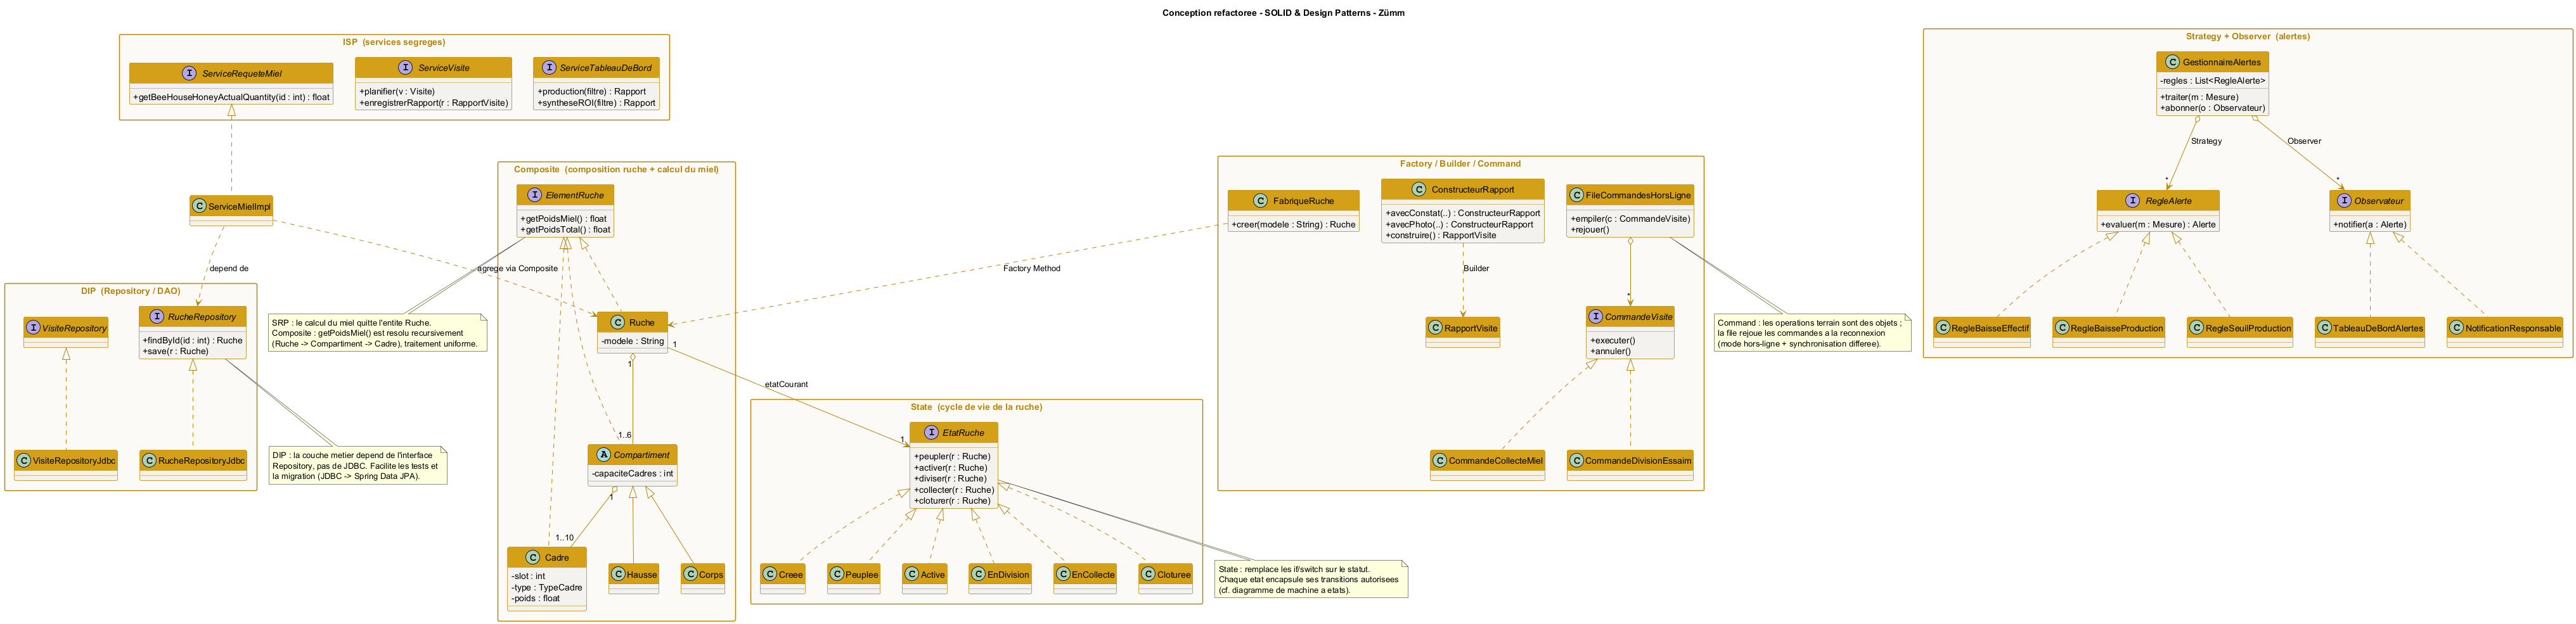
\includegraphics[width=\linewidth]{diagramme_classes_solid}
\caption{Diagramme de classes refactore : application de SOLID et des design
patterns au systeme Z\"umm.}
\label{fig:solid}
\end{figure}

\begin{encadre}
\textbf{Correspondance avec les couches :} les \texttt{Repository} appartiennent
a la couche d'acces aux donnees (JDBC), les \texttt{Service} et le domaine
(Composite, State, Strategy, Observer, Command) a la couche metier (EJB), la
\texttt{Facade} et le \texttt{Proxy} a la couche de controle (Servlets), le
\texttt{Builder} de rapport a la presentation (JSP). L'architecture en couches
faiblement couplees du chapitre~\ref{chap:conception} est ainsi renforcee, sans
etre modifiee.
\end{encadre}
 dans cahier_des_charges.tex
%  (utilise la charte "Miel & noir" : miel, mielfonce, encadre, colonne C,
%   longtable, booktabs -- deja definis dans le preambule principal)
%==============================================================================

%==============================================================================
\chapter{Annexe - Principes SOLID et design patterns}
\label{chap:solid}
%==============================================================================
Cette annexe repond a la question du \emph{comment} de la qualite logicielle.
Elle documente l'application des cinq principes \textbf{SOLID} et d'un ensemble
de \textbf{design patterns} (patrons de conception) au systeme \textbf{Z\"umm},
en mettant chaque decision en regard de la conception initiale (\emph{avant})
et de la conception refactoree (\emph{apres}). L'objectif est une architecture
\textbf{multi-niveaux, evolutive et faiblement couplee}, conforme aux exigences
du chapitre~\ref{chap:conception}.

\begin{encadre}
\textbf{Sources methodologiques :} les definitions retenues suivent la
presentation des principes SOLID de \emph{alexsoyes.com} et le catalogue de
patrons de \emph{refactoring.guru}, adaptes au domaine apicole du projet.
\end{encadre}

%------------------------------------------------------------------------------
\section{Les cinq principes SOLID}
%------------------------------------------------------------------------------
\begin{longtable}{>{\bfseries}p{2.4cm} p{6cm} p{6.2cm}}
\toprule
\textbf{Principe} & \textbf{Avant (conception initiale)} & \textbf{Apres (refactoree)} \\
\midrule
\endhead
S -- Responsabilite unique &
L'entite \texttt{Ruche} porte la methode de calcul
\texttt{getBeeHouseHoneyActualQuantity()} : elle melange l'etat (donnees) et la
logique metier ; \texttt{Visite} regroupe donnees et champs de rapport. &
Le calcul est extrait dans \texttt{ServiceMielImpl} (via le Composite) et le
rapport devient \texttt{RapportVisite}. Chaque classe n'a plus qu'une seule
raison de changer. \\
O -- Ouvert / ferme &
La detection d'alertes et la conversion d'unites reposeraient sur des
\texttt{if / switch} sur \texttt{typeSeuil} et \texttt{unite} : ajouter une
regle ou une unite impose de modifier le code existant. &
\texttt{RegleAlerte} (Strategy) et \texttt{ConvertisseurUnite} : une nouvelle
regle ou unite = une nouvelle classe, sans toucher au \texttt{GestionnaireAlertes}.
Ouvert a l'extension, ferme a la modification. \\
L -- Substitution de Liskov &
Le diagramme de cas d'utilisation generalise l'agent superviseur a partir de
l'agent apiculteur ; transpose tel quel en heritage de classes, un sous-type
restrictif casserait la substituabilite. &
\texttt{Corps} et \texttt{Hausse} heritent de \texttt{Compartiment} en
respectant integralement son contrat (capacite 1..10, \texttt{getPoidsMiel}).
Le role de l'agent passe par l'enumeration \texttt{Role} + permissions
(composition) plutot qu'un heritage restrictif. \\
I -- Segregation des interfaces &
Un service unique \og fourre-tout \fg{} (CRUD + visites + tableaux de bord +
API miel) obligerait l'application tierce a dependre de methodes inutilisees. &
Interfaces ciblees : \texttt{ServiceRequeteMiel} (l'API tierce ne voit que
\texttt{getBeeHouseHoneyActualQuantity}), \texttt{ServiceVisite},
\texttt{ServiceTableauDeBord}. Chaque client ne depend que de son contrat. \\
D -- Inversion de dependance &
La couche metier (EJB) appelle directement JDBC (implementation concrete) :
couplage fort a la base et aux \texttt{ResultSet}. &
La couche metier depend d'abstractions \texttt{RucheRepository} /
\texttt{VisiteRepository} (pattern DAO), implementees par
\texttt{RucheRepositoryJdbc}. Tests par mock et migration JDBC \textrightarrow{}
Spring Data JPA facilites (cf. annexe~\ref{chap:migration}). \\
\bottomrule
\end{longtable}

%------------------------------------------------------------------------------
\section{Design patterns retenus}
%------------------------------------------------------------------------------
Le tableau suivant recense les patrons appliques, leur categorie (creationnel,
structurel, comportemental) et la couche concernee, avec la justification
\emph{avant / apres}.

\begin{longtable}{>{\bfseries}p{2.7cm} p{5.9cm} p{6.2cm}}
\toprule
\textbf{Pattern} & \textbf{Avant} & \textbf{Apres} \\
\midrule
\endhead
Composite \newline {\small\itshape structurel -- metier} &
Le calcul du miel parcourt manuellement les collections de cadres avec du code
de sommation duplique. &
\texttt{ElementRuche.getPoidsMiel()} est resolu recursivement
(Ruche \textrightarrow{} Compartiment \textrightarrow{} Cadre) : traitement
uniforme de l'arborescence. \\
State \newline {\small\itshape comportemental -- metier} &
Le statut de la ruche serait teste par des \texttt{switch} disperses (creee,
active, en collecte, cloturee, \ldots). &
\texttt{EtatRuche} et ses etats concrets encapsulent les transitions autorisees ;
alignement direct sur le diagramme de machine a etats. \\
Strategy \newline {\small\itshape comportemental -- metier} &
Les regles d'alerte, la conversion d'unites et le ROI seraient codes en dur. &
Familles d'algorithmes interchangeables (\texttt{RegleAlerte},
\texttt{ConvertisseurUnite}), injectables et testables isolement. \\
Observer \newline {\small\itshape comportemental -- metier} &
Le code de mesure appellerait directement les tableaux de bord (couplage fort). &
\texttt{GestionnaireAlertes} notifie les \texttt{Observateur} abonnes (tableau
de bord d'alertes, notification du responsable) au franchissement d'un seuil. \\
Command \newline {\small\itshape comportemental -- controle} &
Les operations terrain (collecte, division, changement de reine) sont des appels
directs, non rejouables hors-ligne. &
Chaque operation devient une \texttt{CommandeVisite} ; la
\texttt{FileCommandesHorsLigne} rejoue les commandes a la reconnexion
(mode hors-ligne + synchronisation differee). \\
Factory Method \newline {\small\itshape creationnel -- metier} &
Les ruches sont creees par des \texttt{new} disperses avec initialisation
manuelle des compartiments. &
\texttt{FabriqueRuche.creer(modele)} produit une ruche preconfiguree selon le
modele (Dadant, Langstroth\ldots) avec corps et capacites coherents. \\
Builder \newline {\small\itshape creationnel -- presentation} &
Le rapport de visite, aux nombreux champs optionnels, imposerait un constructeur
telescopique ou des setters epars. &
\texttt{ConstructeurRapport} construit \texttt{RapportVisite} de facon fluide
(constatations, actions, photos, evaluations). \\
Adapter \newline {\small\itshape structurel -- donnees} &
Les capteurs heterogenes (formats et unites differents) seraient traites au cas
par cas. &
\texttt{AdaptateurCapteur} uniformise chaque source en \texttt{Mesure} avec
unites parametrables (volet automatise). \\
Facade \newline {\small\itshape structurel -- controle} &
Le Servlet orchestre directement tous les services metier. &
\texttt{FacadeApplication} offre un point d'entree simplifie aux Servlets
par-dessus les sous-systemes. \\
Singleton \newline {\small\itshape creationnel -- transverse} &
Le fichier \texttt{ConfigBKS.ini} et les libelles i18n seraient relus en
plusieurs instances. &
\texttt{Configuration} et \texttt{GestionnaireI18n} garantissent une instance
unique partagee. \\
Proxy \newline {\small\itshape structurel -- services web} &
L'acces a l'API exposerait directement le service metier. &
Un \texttt{ProxySecurite} controle l'authentification OAuth et le chiffrement
SSL / X.509 avant de deleguer au service. \\
\bottomrule
\end{longtable}

%------------------------------------------------------------------------------
\section{Vue de conception refactoree}
%------------------------------------------------------------------------------
La figure~\ref{fig:solid} synthetise les principaux patrons dans un diagramme
de classes de conception : le Composite (composition de la ruche et calcul du
miel), le State (cycle de vie), les services segreges (ISP), la persistance par
abstraction (DIP / Repository), le couple Strategy + Observer (alertes) et le
trio Factory / Builder / Command.

\begin{figure}[htbp]
\centering
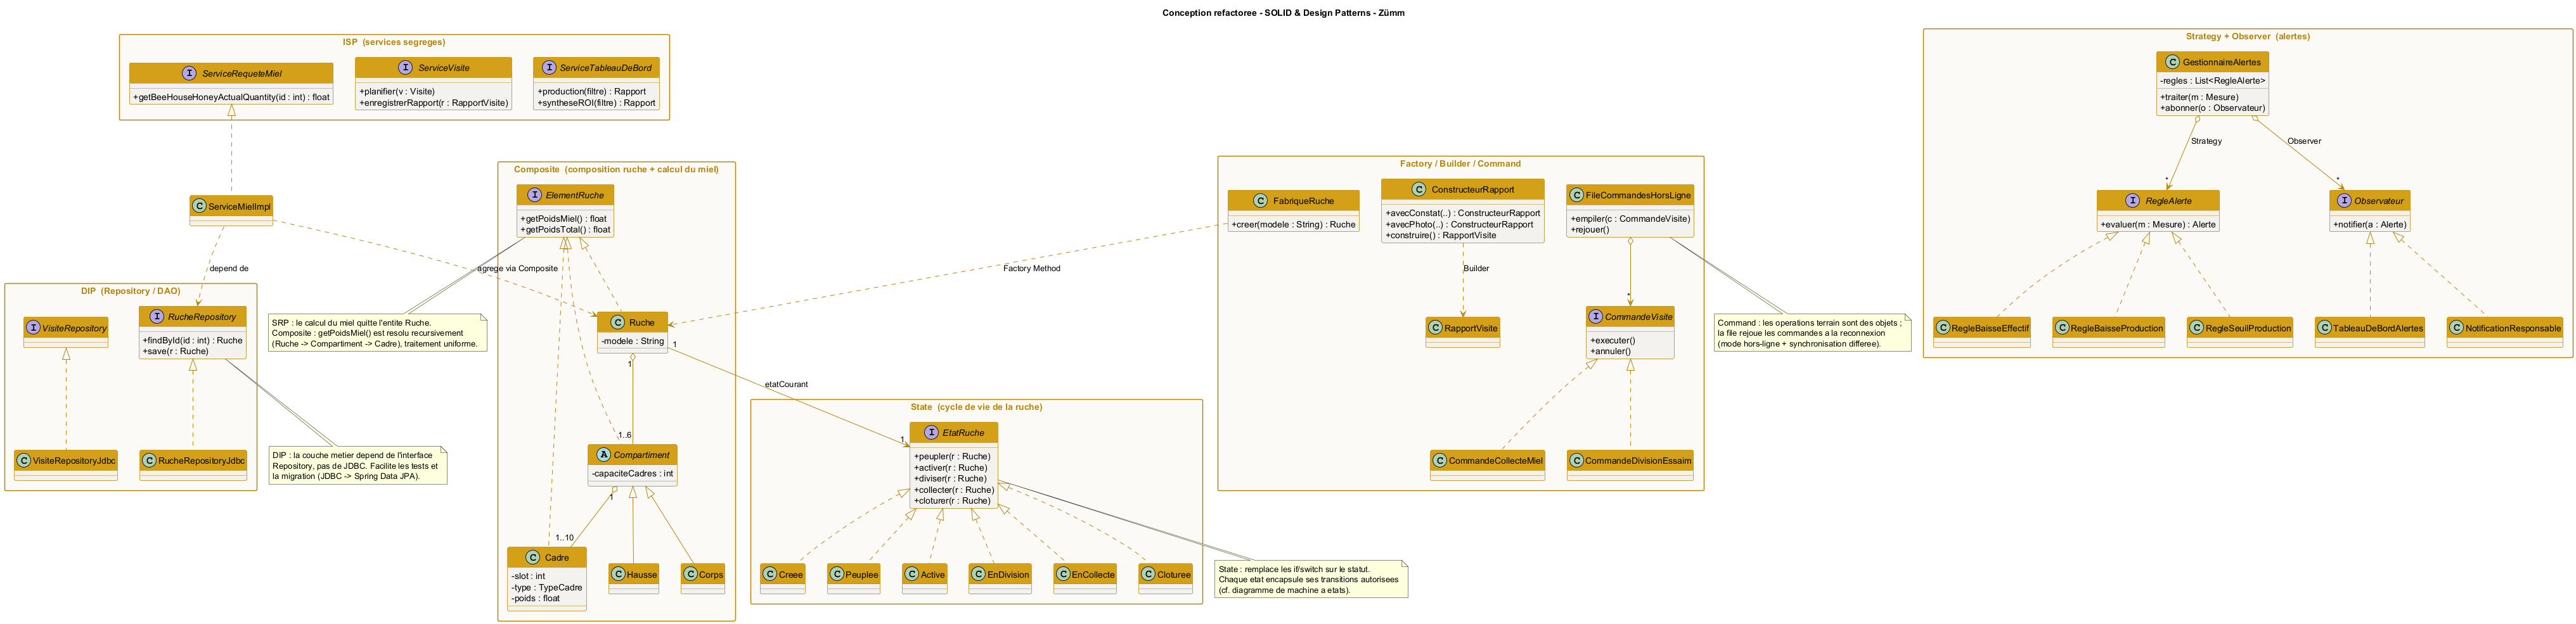
\includegraphics[width=\linewidth]{diagramme_classes_solid}
\caption{Diagramme de classes refactore : application de SOLID et des design
patterns au systeme Z\"umm.}
\label{fig:solid}
\end{figure}

\begin{encadre}
\textbf{Correspondance avec les couches :} les \texttt{Repository} appartiennent
a la couche d'acces aux donnees (JDBC), les \texttt{Service} et le domaine
(Composite, State, Strategy, Observer, Command) a la couche metier (EJB), la
\texttt{Facade} et le \texttt{Proxy} a la couche de controle (Servlets), le
\texttt{Builder} de rapport a la presentation (JSP). L'architecture en couches
faiblement couplees du chapitre~\ref{chap:conception} est ainsi renforcee, sans
etre modifiee.
\end{encadre}
 dans cahier_des_charges.tex
%  (utilise la charte "Miel & noir" : miel, mielfonce, encadre, colonne C,
%   longtable, booktabs -- deja definis dans le preambule principal)
%==============================================================================

%==============================================================================
\chapter{Annexe - Principes SOLID et design patterns}
\label{chap:solid}
%==============================================================================
Cette annexe repond a la question du \emph{comment} de la qualite logicielle.
Elle documente l'application des cinq principes \textbf{SOLID} et d'un ensemble
de \textbf{design patterns} (patrons de conception) au systeme \textbf{Z\"umm},
en mettant chaque decision en regard de la conception initiale (\emph{avant})
et de la conception refactoree (\emph{apres}). L'objectif est une architecture
\textbf{multi-niveaux, evolutive et faiblement couplee}, conforme aux exigences
du chapitre~\ref{chap:conception}.

\begin{encadre}
\textbf{Sources methodologiques :} les definitions retenues suivent la
presentation des principes SOLID de \emph{alexsoyes.com} et le catalogue de
patrons de \emph{refactoring.guru}, adaptes au domaine apicole du projet.
\end{encadre}

%------------------------------------------------------------------------------
\section{Les cinq principes SOLID}
%------------------------------------------------------------------------------
\begin{longtable}{>{\bfseries}p{2.4cm} p{6cm} p{6.2cm}}
\toprule
\textbf{Principe} & \textbf{Avant (conception initiale)} & \textbf{Apres (refactoree)} \\
\midrule
\endhead
S -- Responsabilite unique &
L'entite \texttt{Ruche} porte la methode de calcul
\texttt{getBeeHouseHoneyActualQuantity()} : elle melange l'etat (donnees) et la
logique metier ; \texttt{Visite} regroupe donnees et champs de rapport. &
Le calcul est extrait dans \texttt{ServiceMielImpl} (via le Composite) et le
rapport devient \texttt{RapportVisite}. Chaque classe n'a plus qu'une seule
raison de changer. \\
O -- Ouvert / ferme &
La detection d'alertes et la conversion d'unites reposeraient sur des
\texttt{if / switch} sur \texttt{typeSeuil} et \texttt{unite} : ajouter une
regle ou une unite impose de modifier le code existant. &
\texttt{RegleAlerte} (Strategy) et \texttt{ConvertisseurUnite} : une nouvelle
regle ou unite = une nouvelle classe, sans toucher au \texttt{GestionnaireAlertes}.
Ouvert a l'extension, ferme a la modification. \\
L -- Substitution de Liskov &
Le diagramme de cas d'utilisation generalise l'agent superviseur a partir de
l'agent apiculteur ; transpose tel quel en heritage de classes, un sous-type
restrictif casserait la substituabilite. &
\texttt{Corps} et \texttt{Hausse} heritent de \texttt{Compartiment} en
respectant integralement son contrat (capacite 1..10, \texttt{getPoidsMiel}).
Le role de l'agent passe par l'enumeration \texttt{Role} + permissions
(composition) plutot qu'un heritage restrictif. \\
I -- Segregation des interfaces &
Un service unique \og fourre-tout \fg{} (CRUD + visites + tableaux de bord +
API miel) obligerait l'application tierce a dependre de methodes inutilisees. &
Interfaces ciblees : \texttt{ServiceRequeteMiel} (l'API tierce ne voit que
\texttt{getBeeHouseHoneyActualQuantity}), \texttt{ServiceVisite},
\texttt{ServiceTableauDeBord}. Chaque client ne depend que de son contrat. \\
D -- Inversion de dependance &
La couche metier (EJB) appelle directement JDBC (implementation concrete) :
couplage fort a la base et aux \texttt{ResultSet}. &
La couche metier depend d'abstractions \texttt{RucheRepository} /
\texttt{VisiteRepository} (pattern DAO), implementees par
\texttt{RucheRepositoryJdbc}. Tests par mock et migration JDBC \textrightarrow{}
Spring Data JPA facilites (cf. annexe~\ref{chap:migration}). \\
\bottomrule
\end{longtable}

%------------------------------------------------------------------------------
\section{Design patterns retenus}
%------------------------------------------------------------------------------
Le tableau suivant recense les patrons appliques, leur categorie (creationnel,
structurel, comportemental) et la couche concernee, avec la justification
\emph{avant / apres}.

\begin{longtable}{>{\bfseries}p{2.7cm} p{5.9cm} p{6.2cm}}
\toprule
\textbf{Pattern} & \textbf{Avant} & \textbf{Apres} \\
\midrule
\endhead
Composite \newline {\small\itshape structurel -- metier} &
Le calcul du miel parcourt manuellement les collections de cadres avec du code
de sommation duplique. &
\texttt{ElementRuche.getPoidsMiel()} est resolu recursivement
(Ruche \textrightarrow{} Compartiment \textrightarrow{} Cadre) : traitement
uniforme de l'arborescence. \\
State \newline {\small\itshape comportemental -- metier} &
Le statut de la ruche serait teste par des \texttt{switch} disperses (creee,
active, en collecte, cloturee, \ldots). &
\texttt{EtatRuche} et ses etats concrets encapsulent les transitions autorisees ;
alignement direct sur le diagramme de machine a etats. \\
Strategy \newline {\small\itshape comportemental -- metier} &
Les regles d'alerte, la conversion d'unites et le ROI seraient codes en dur. &
Familles d'algorithmes interchangeables (\texttt{RegleAlerte},
\texttt{ConvertisseurUnite}), injectables et testables isolement. \\
Observer \newline {\small\itshape comportemental -- metier} &
Le code de mesure appellerait directement les tableaux de bord (couplage fort). &
\texttt{GestionnaireAlertes} notifie les \texttt{Observateur} abonnes (tableau
de bord d'alertes, notification du responsable) au franchissement d'un seuil. \\
Command \newline {\small\itshape comportemental -- controle} &
Les operations terrain (collecte, division, changement de reine) sont des appels
directs, non rejouables hors-ligne. &
Chaque operation devient une \texttt{CommandeVisite} ; la
\texttt{FileCommandesHorsLigne} rejoue les commandes a la reconnexion
(mode hors-ligne + synchronisation differee). \\
Factory Method \newline {\small\itshape creationnel -- metier} &
Les ruches sont creees par des \texttt{new} disperses avec initialisation
manuelle des compartiments. &
\texttt{FabriqueRuche.creer(modele)} produit une ruche preconfiguree selon le
modele (Dadant, Langstroth\ldots) avec corps et capacites coherents. \\
Builder \newline {\small\itshape creationnel -- presentation} &
Le rapport de visite, aux nombreux champs optionnels, imposerait un constructeur
telescopique ou des setters epars. &
\texttt{ConstructeurRapport} construit \texttt{RapportVisite} de facon fluide
(constatations, actions, photos, evaluations). \\
Adapter \newline {\small\itshape structurel -- donnees} &
Les capteurs heterogenes (formats et unites differents) seraient traites au cas
par cas. &
\texttt{AdaptateurCapteur} uniformise chaque source en \texttt{Mesure} avec
unites parametrables (volet automatise). \\
Facade \newline {\small\itshape structurel -- controle} &
Le Servlet orchestre directement tous les services metier. &
\texttt{FacadeApplication} offre un point d'entree simplifie aux Servlets
par-dessus les sous-systemes. \\
Singleton \newline {\small\itshape creationnel -- transverse} &
Le fichier \texttt{ConfigBKS.ini} et les libelles i18n seraient relus en
plusieurs instances. &
\texttt{Configuration} et \texttt{GestionnaireI18n} garantissent une instance
unique partagee. \\
Proxy \newline {\small\itshape structurel -- services web} &
L'acces a l'API exposerait directement le service metier. &
Un \texttt{ProxySecurite} controle l'authentification OAuth et le chiffrement
SSL / X.509 avant de deleguer au service. \\
\bottomrule
\end{longtable}

%------------------------------------------------------------------------------
\section{Vue de conception refactoree}
%------------------------------------------------------------------------------
La figure~\ref{fig:solid} synthetise les principaux patrons dans un diagramme
de classes de conception : le Composite (composition de la ruche et calcul du
miel), le State (cycle de vie), les services segreges (ISP), la persistance par
abstraction (DIP / Repository), le couple Strategy + Observer (alertes) et le
trio Factory / Builder / Command.

\begin{figure}[htbp]
\centering
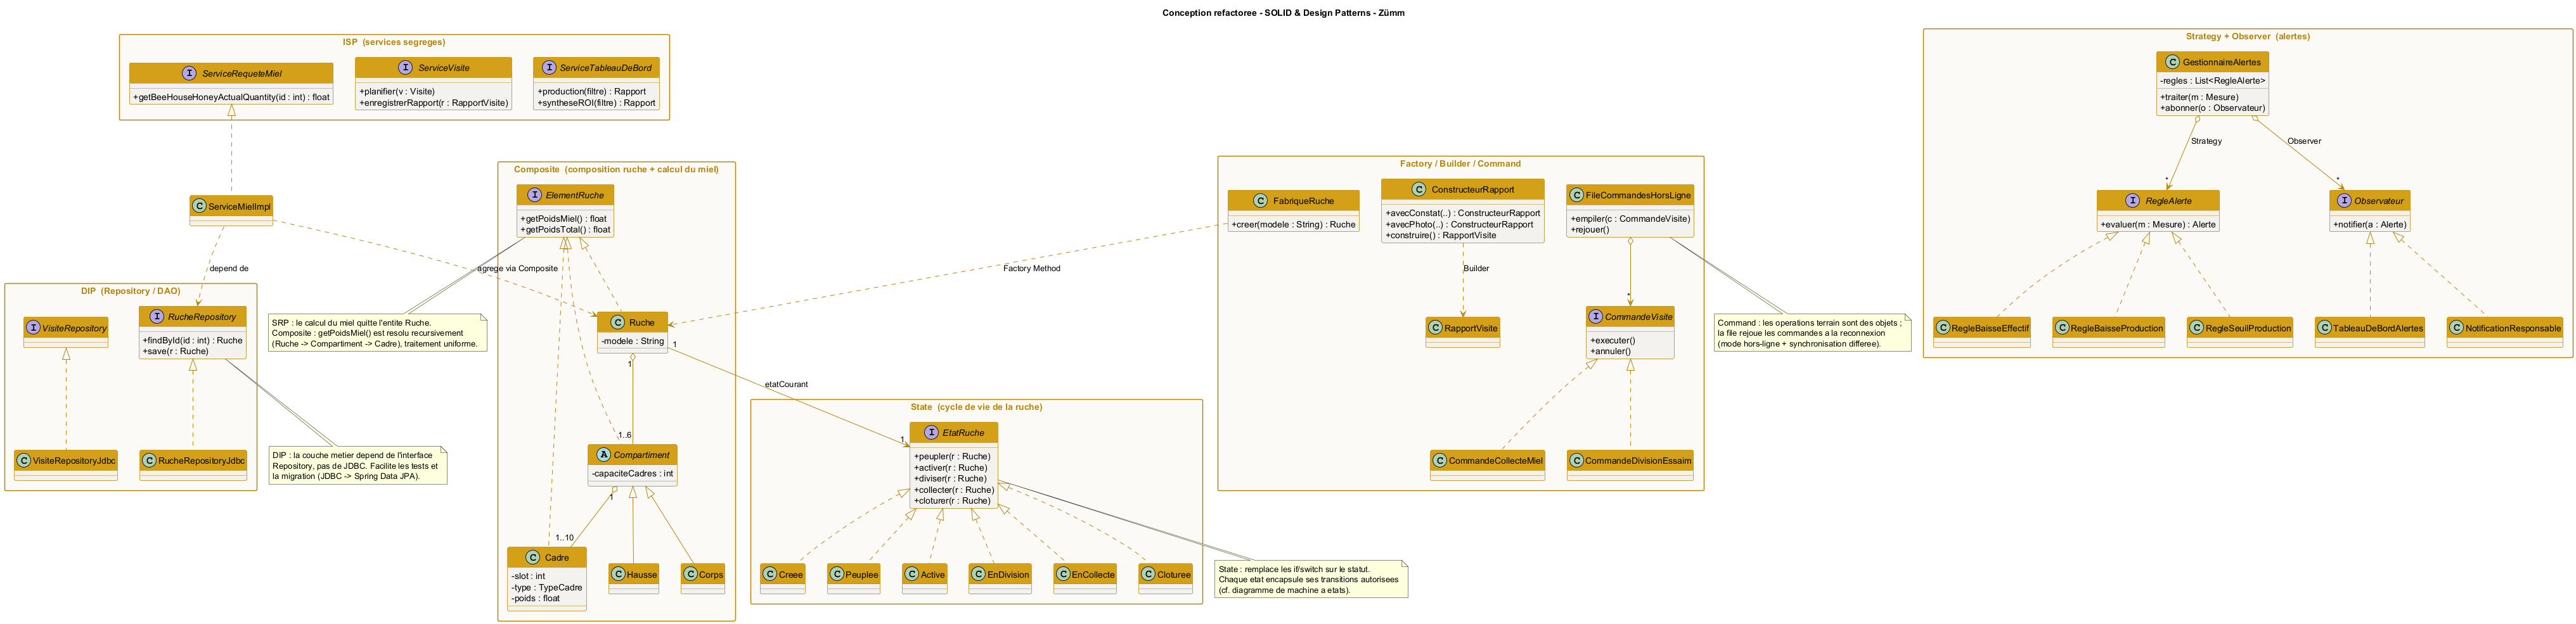
\includegraphics[width=\linewidth]{diagramme_classes_solid}
\caption{Diagramme de classes refactore : application de SOLID et des design
patterns au systeme Z\"umm.}
\label{fig:solid}
\end{figure}

\begin{encadre}
\textbf{Correspondance avec les couches :} les \texttt{Repository} appartiennent
a la couche d'acces aux donnees (JDBC), les \texttt{Service} et le domaine
(Composite, State, Strategy, Observer, Command) a la couche metier (EJB), la
\texttt{Facade} et le \texttt{Proxy} a la couche de controle (Servlets), le
\texttt{Builder} de rapport a la presentation (JSP). L'architecture en couches
faiblement couplees du chapitre~\ref{chap:conception} est ainsi renforcee, sans
etre modifiee.
\end{encadre}


%==============================================================================
%  ANNEXE - Complements : donnees, IHM, securite et tests
%  A inserer via %==============================================================================
%  ANNEXE - Complements : donnees, IHM, securite et tests
%  A inserer via %==============================================================================
%  ANNEXE - Complements : donnees, IHM, securite et tests
%  A inserer via \input{annexe_complements} dans cahier_des_charges.tex
%  (charte "Miel & noir" : miel, mielfonce, encadre, colonne C, longtable,
%   booktabs -- deja definis dans le preambule principal)
%==============================================================================

%==============================================================================
\chapter{Annexe - Complements : donnees, IHM, securite et tests}
\label{chap:complements}
%==============================================================================
Cette annexe regroupe des livrables complementaires renforcant le dossier :
le modele logique de donnees, les maquettes de l'interface, la matrice des
droits d'acces, le registre des risques, la conformite a la protection des
donnees et la strategie de tests.

%------------------------------------------------------------------------------
\section{Modele logique de donnees (MLD)}
%------------------------------------------------------------------------------
Le MLD traduit le dictionnaire de donnees (chapitre~5) en tables relationnelles
avec cles primaires, cles etrangeres et contraintes de gestion (\texttt{CHECK}
sur le nombre de hausses, la capacite en cadres et la productivite ; unicite du
couple compartiment/slot). Il distingue la relation d'\emph{emplacement}
(un site heberge des ruches) de la relation de \emph{propriete} (une ferme
possede des ruches), conformement a la regle autorisant un site a accueillir des
ruches de plusieurs fermes.

\begin{figure}[htbp]
\centering
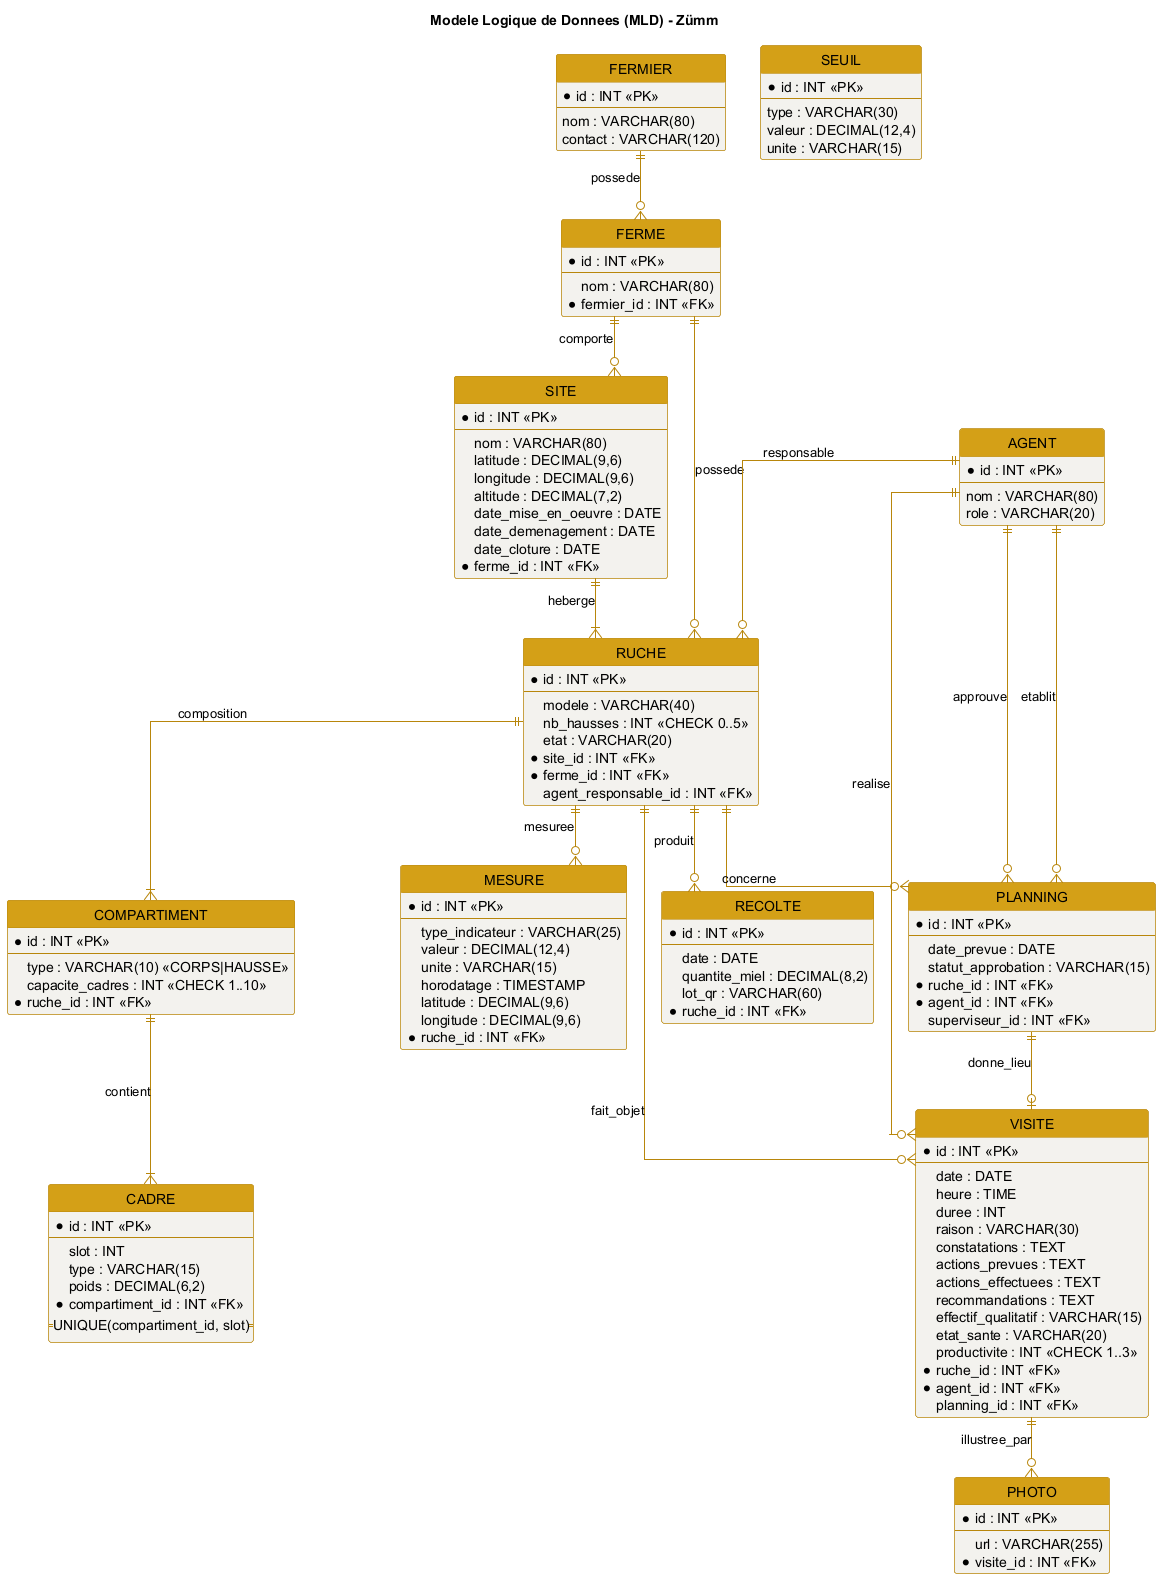
\includegraphics[width=0.82\linewidth]{diagramme_mld}
\caption{Modele logique de donnees relationnel du systeme Z\"umm.}
\label{fig:mld}
\end{figure}

%------------------------------------------------------------------------------
\section{Maquettes de l'interface (wireframes)}
%------------------------------------------------------------------------------
Les maquettes basse-fidelite suivantes fixent l'ergonomie des ecrans cles avant
le developpement. Elles respectent la charte visuelle et la simplicite exigee.

\begin{figure}[htbp]
\centering
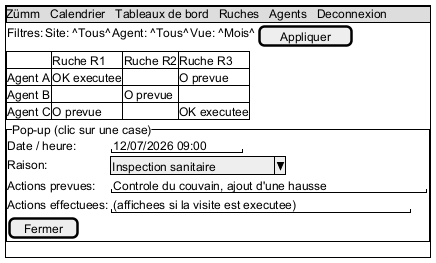
\includegraphics[width=0.9\linewidth]{wireframe_calendrier}
\caption{Maquette : calendrier / matrice agents x ruches avec pop-up de visite.}
\label{fig:wf-calendrier}
\end{figure}

\begin{figure}[htbp]
\centering
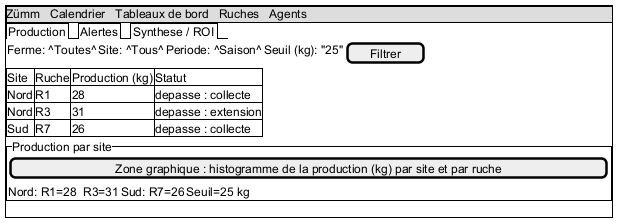
\includegraphics[width=0.9\linewidth]{wireframe_tdb_production}
\caption{Maquette : tableau de bord de production avec seuil parametrable.}
\label{fig:wf-production}
\end{figure}

\begin{figure}[htbp]
\centering
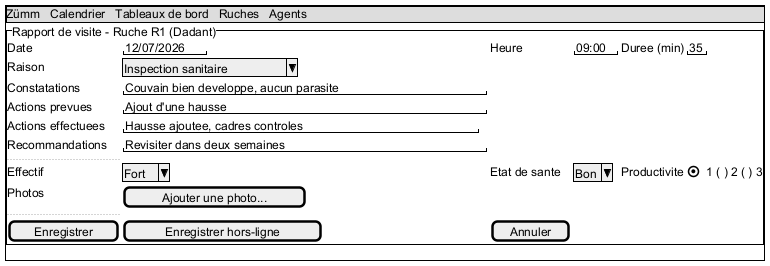
\includegraphics[width=0.95\linewidth]{wireframe_rapport_visite}
\caption{Maquette : formulaire de rapport de visite (avec mode hors-ligne et photos).}
\label{fig:wf-rapport}
\end{figure}

\begin{figure}[htbp]
\centering
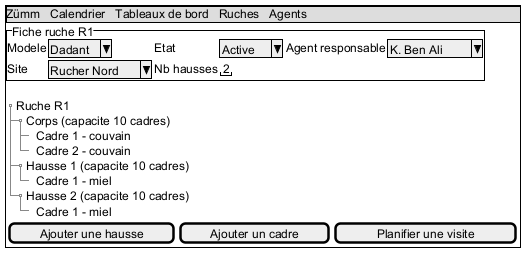
\includegraphics[width=0.85\linewidth]{wireframe_ruche}
\caption{Maquette : fiche d'une ruche et composition (corps, hausses, cadres).}
\label{fig:wf-ruche}
\end{figure}

%------------------------------------------------------------------------------
\section{Matrice des droits d'acces (RBAC)}
%------------------------------------------------------------------------------
La matrice precise, pour chaque fonction, le droit accorde a chaque profil.
\textbf{Legende :} CRUD = creation / lecture / mise a jour / suppression ;
R = lecture ; X = execution ; A = approbation ; --- = aucun acces.

\begin{longtable}{>{\bfseries}p{3.6cm} C{1.3cm} C{1.3cm} C{1.3cm} C{1.3cm} C{1.3cm} C{1.3cm}}
\toprule
\textbf{Fonction} & \textbf{Prop.} & \textbf{Apic.} & \textbf{Sup.} & \textbf{Resp.} & \textbf{Admin} & \textbf{API} \\
\midrule
\endhead
Fermes et sites          & CRUD & R    & R    & R    & CRUD & --- \\
Ruches (corps/cadres)    & CRUD & R    & R    & R    & CRUD & --- \\
Agents                   & R    & ---  & R    & R    & CRUD & --- \\
Planifier une visite     & R    & X    & X    & X    & X    & --- \\
Approuver le planning    & ---  & ---  & A    & ---  & X    & --- \\
Realiser visite/rapport  & R    & X    & X    & ---  & R    & --- \\
Calendrier agents x ruches & R  & R    & R    & R    & R    & --- \\
TB production            & R    & ---  & ---  & R    & R    & --- \\
TB alertes / traiter     & R    & ---  & ---  & X    & R    & --- \\
Synthese et ROI          & R    & ---  & ---  & R    & R    & --- \\
Parametrer seuils/unites & ---  & ---  & ---  & R    & CRUD & --- \\
Internationalisation     & ---  & ---  & ---  & ---  & CRUD & --- \\
Export CSV / TXT         & R    & R    & R    & R    & R    & --- \\
Sauvegarde / restauration & --- & ---  & ---  & ---  & X    & --- \\
API quantite de miel     & ---  & ---  & ---  & ---  & ---  & R \\
\bottomrule
\end{longtable}

\begin{encadre}
Cette matrice doit etre appliquee cote serveur (verification systematique des
droits dans la couche de controle), et non uniquement par le masquage des
elements d'interface.
\end{encadre}

%------------------------------------------------------------------------------
\section{Registre des risques}
%------------------------------------------------------------------------------
\begin{longtable}{>{\bfseries}p{4.6cm} C{1.8cm} C{1.6cm} p{5.4cm}}
\toprule
\textbf{Risque} & \textbf{Probab.} & \textbf{Impact} & \textbf{Mesure de reduction} \\
\midrule
\endhead
Retard de developpement       & Moyenne & Fort      & Prioriser le noyau CRUD ; jalons hebdomadaires (S5 a S12). \\
Portee trop large             & Moyenne & Fort      & Se limiter aux fonctions de priorite haute ; le reste en option. \\
Complexite i18n arabe (RTL)   & Moyenne & Moyen     & Test precoce de bout en bout FR/EN/AR, gestion \texttt{dir=rtl}. \\
Perte de donnees terrain      & Moyenne & Fort      & File de commandes hors-ligne + synchronisation + sauvegarde. \\
Failles applicatives (injection, XSS) & Moyenne & Fort & \texttt{PreparedStatement}, echappement JSP, revue de securite. \\
Fausses alertes (capteurs)    & Moyenne & Moyen     & Seuils parametrables + validation humaine par le rapport. \\
Indisponibilite d'OAuth Google & Faible & Moyen     & Repli d'authentification locale pour la demonstration. \\
Volumetrie des mesures        & Faible  & Moyen     & Archivage et agregation par periode (volet automatise). \\
Usage d'un generateur de code & Faible  & Tres fort & Conception et code faits maison, tracabilite et revue par pairs. \\
\bottomrule
\end{longtable}

%------------------------------------------------------------------------------
\section{Protection des donnees personnelles}
%------------------------------------------------------------------------------
Le systeme manipule des donnees personnelles (noms et contacts des fermiers et
des agents) et des donnees potentiellement sensibles (\textbf{geolocalisation}
precise des sites). Les principes suivants sont retenus, dans l'esprit du RGPD :
\begin{itemize}
  \item \textbf{Minimisation et finalite} : ne collecter que les donnees utiles au suivi apicole.
  \item \textbf{Securite} : chiffrement des echanges (SSL / X.509) et acces authentifies, deja prevus.
  \item \textbf{Controle d'acces} : application stricte de la matrice RBAC ci-dessus.
  \item \textbf{Droits des personnes} : consultation, rectification et \textbf{effacement} des donnees, \textbf{portabilite} assuree par l'export CSV / TXT.
  \item \textbf{Conservation} : duree de retention definie pour les mesures et les visites, au-dela de laquelle les donnees sont archivees ou anonymisees.
  \item \textbf{Tracabilite} : journalisation des acces et des actions sensibles (approbation de planning, cloture de site).
\end{itemize}

%------------------------------------------------------------------------------
\section{Strategie de tests}
%------------------------------------------------------------------------------
La strategie complete le plan de tests fonctionnels (chapitre~10) par les
niveaux unitaire et d'integration. La conception faiblement couplee (interfaces
\texttt{Repository}, services segreges) rend les regles metier testables en
isolation, par injection de doubles (mocks).

\begin{longtable}{>{\bfseries}p{2.8cm} p{4.4cm} p{4.4cm} C{2.2cm}}
\toprule
\textbf{Niveau} & \textbf{Portee} & \textbf{Exemples} & \textbf{Outil} \\
\midrule
\endhead
Unitaire      & Regles de gestion isolees          & Contraintes cadres/hausses, calcul du miel (Composite), ROI, seuils & JUnit 5, Mockito \\
Integration   & Acces aux donnees (Repository/JDBC) & CRUD persiste, requetes de calcul                                   & JUnit + base H2 \\
Systeme       & Cas fonctionnels de bout en bout    & Cas TC01 a TC16 du chapitre~10                                      & JUnit, Selenium \\
Acceptation   & Validation par la demonstration     & Parcours agent, fermier, responsable                                & Soutenance \\
\bottomrule
\end{longtable}

\begin{itemize}
  \item \textbf{Couverture visee} : au moins 70\,\% de la couche metier (regles de gestion), mesuree par \texttt{JaCoCo}.
  \item \textbf{Tracabilite} : chaque exigence est reliee a au moins un cas de test (matrice du chapitre~10), completee par les tests unitaires correspondants.
  \item \textbf{Automatisation} : execution des tests a chaque build (Maven), pre-requis a la livraison.
\end{itemize}

\begin{encadre}
\textbf{Synergie avec la conception :} l'inversion de dependance (DIP) permet de
substituer un \texttt{RucheRepository} en memoire aux implementations JDBC, ce
qui rend les tests rapides, deterministes et independants de la base.
\end{encadre}
 dans cahier_des_charges.tex
%  (charte "Miel & noir" : miel, mielfonce, encadre, colonne C, longtable,
%   booktabs -- deja definis dans le preambule principal)
%==============================================================================

%==============================================================================
\chapter{Annexe - Complements : donnees, IHM, securite et tests}
\label{chap:complements}
%==============================================================================
Cette annexe regroupe des livrables complementaires renforcant le dossier :
le modele logique de donnees, les maquettes de l'interface, la matrice des
droits d'acces, le registre des risques, la conformite a la protection des
donnees et la strategie de tests.

%------------------------------------------------------------------------------
\section{Modele logique de donnees (MLD)}
%------------------------------------------------------------------------------
Le MLD traduit le dictionnaire de donnees (chapitre~5) en tables relationnelles
avec cles primaires, cles etrangeres et contraintes de gestion (\texttt{CHECK}
sur le nombre de hausses, la capacite en cadres et la productivite ; unicite du
couple compartiment/slot). Il distingue la relation d'\emph{emplacement}
(un site heberge des ruches) de la relation de \emph{propriete} (une ferme
possede des ruches), conformement a la regle autorisant un site a accueillir des
ruches de plusieurs fermes.

\begin{figure}[htbp]
\centering
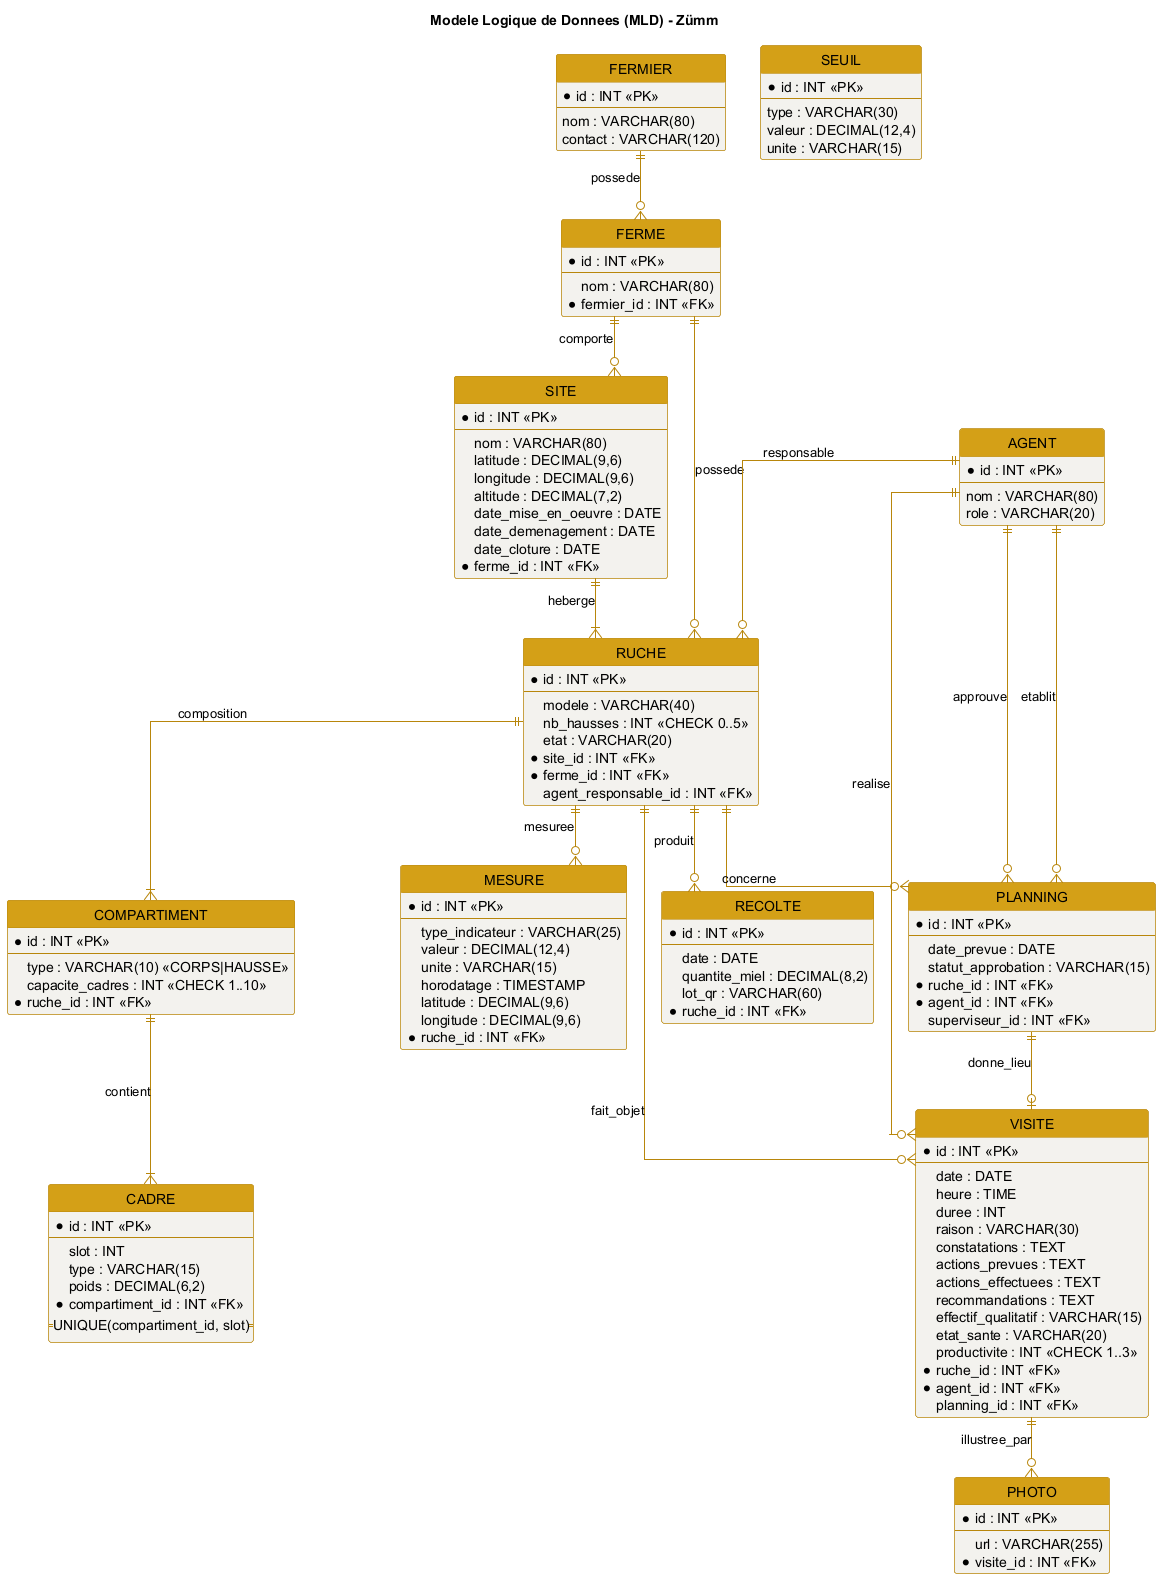
\includegraphics[width=0.82\linewidth]{diagramme_mld}
\caption{Modele logique de donnees relationnel du systeme Z\"umm.}
\label{fig:mld}
\end{figure}

%------------------------------------------------------------------------------
\section{Maquettes de l'interface (wireframes)}
%------------------------------------------------------------------------------
Les maquettes basse-fidelite suivantes fixent l'ergonomie des ecrans cles avant
le developpement. Elles respectent la charte visuelle et la simplicite exigee.

\begin{figure}[htbp]
\centering
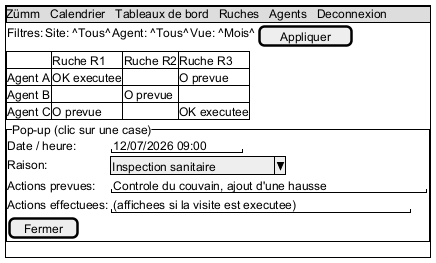
\includegraphics[width=0.9\linewidth]{wireframe_calendrier}
\caption{Maquette : calendrier / matrice agents x ruches avec pop-up de visite.}
\label{fig:wf-calendrier}
\end{figure}

\begin{figure}[htbp]
\centering
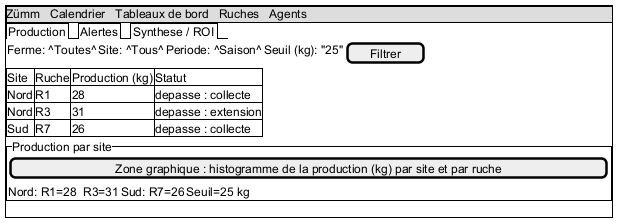
\includegraphics[width=0.9\linewidth]{wireframe_tdb_production}
\caption{Maquette : tableau de bord de production avec seuil parametrable.}
\label{fig:wf-production}
\end{figure}

\begin{figure}[htbp]
\centering
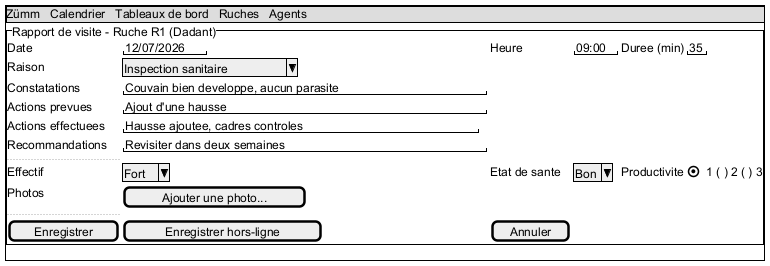
\includegraphics[width=0.95\linewidth]{wireframe_rapport_visite}
\caption{Maquette : formulaire de rapport de visite (avec mode hors-ligne et photos).}
\label{fig:wf-rapport}
\end{figure}

\begin{figure}[htbp]
\centering
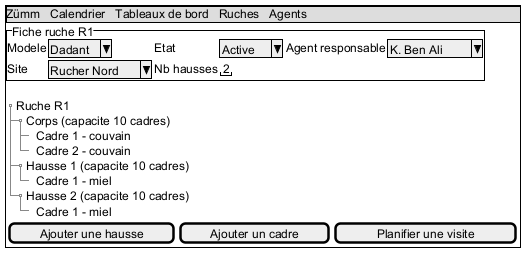
\includegraphics[width=0.85\linewidth]{wireframe_ruche}
\caption{Maquette : fiche d'une ruche et composition (corps, hausses, cadres).}
\label{fig:wf-ruche}
\end{figure}

%------------------------------------------------------------------------------
\section{Matrice des droits d'acces (RBAC)}
%------------------------------------------------------------------------------
La matrice precise, pour chaque fonction, le droit accorde a chaque profil.
\textbf{Legende :} CRUD = creation / lecture / mise a jour / suppression ;
R = lecture ; X = execution ; A = approbation ; --- = aucun acces.

\begin{longtable}{>{\bfseries}p{3.6cm} C{1.3cm} C{1.3cm} C{1.3cm} C{1.3cm} C{1.3cm} C{1.3cm}}
\toprule
\textbf{Fonction} & \textbf{Prop.} & \textbf{Apic.} & \textbf{Sup.} & \textbf{Resp.} & \textbf{Admin} & \textbf{API} \\
\midrule
\endhead
Fermes et sites          & CRUD & R    & R    & R    & CRUD & --- \\
Ruches (corps/cadres)    & CRUD & R    & R    & R    & CRUD & --- \\
Agents                   & R    & ---  & R    & R    & CRUD & --- \\
Planifier une visite     & R    & X    & X    & X    & X    & --- \\
Approuver le planning    & ---  & ---  & A    & ---  & X    & --- \\
Realiser visite/rapport  & R    & X    & X    & ---  & R    & --- \\
Calendrier agents x ruches & R  & R    & R    & R    & R    & --- \\
TB production            & R    & ---  & ---  & R    & R    & --- \\
TB alertes / traiter     & R    & ---  & ---  & X    & R    & --- \\
Synthese et ROI          & R    & ---  & ---  & R    & R    & --- \\
Parametrer seuils/unites & ---  & ---  & ---  & R    & CRUD & --- \\
Internationalisation     & ---  & ---  & ---  & ---  & CRUD & --- \\
Export CSV / TXT         & R    & R    & R    & R    & R    & --- \\
Sauvegarde / restauration & --- & ---  & ---  & ---  & X    & --- \\
API quantite de miel     & ---  & ---  & ---  & ---  & ---  & R \\
\bottomrule
\end{longtable}

\begin{encadre}
Cette matrice doit etre appliquee cote serveur (verification systematique des
droits dans la couche de controle), et non uniquement par le masquage des
elements d'interface.
\end{encadre}

%------------------------------------------------------------------------------
\section{Registre des risques}
%------------------------------------------------------------------------------
\begin{longtable}{>{\bfseries}p{4.6cm} C{1.8cm} C{1.6cm} p{5.4cm}}
\toprule
\textbf{Risque} & \textbf{Probab.} & \textbf{Impact} & \textbf{Mesure de reduction} \\
\midrule
\endhead
Retard de developpement       & Moyenne & Fort      & Prioriser le noyau CRUD ; jalons hebdomadaires (S5 a S12). \\
Portee trop large             & Moyenne & Fort      & Se limiter aux fonctions de priorite haute ; le reste en option. \\
Complexite i18n arabe (RTL)   & Moyenne & Moyen     & Test precoce de bout en bout FR/EN/AR, gestion \texttt{dir=rtl}. \\
Perte de donnees terrain      & Moyenne & Fort      & File de commandes hors-ligne + synchronisation + sauvegarde. \\
Failles applicatives (injection, XSS) & Moyenne & Fort & \texttt{PreparedStatement}, echappement JSP, revue de securite. \\
Fausses alertes (capteurs)    & Moyenne & Moyen     & Seuils parametrables + validation humaine par le rapport. \\
Indisponibilite d'OAuth Google & Faible & Moyen     & Repli d'authentification locale pour la demonstration. \\
Volumetrie des mesures        & Faible  & Moyen     & Archivage et agregation par periode (volet automatise). \\
Usage d'un generateur de code & Faible  & Tres fort & Conception et code faits maison, tracabilite et revue par pairs. \\
\bottomrule
\end{longtable}

%------------------------------------------------------------------------------
\section{Protection des donnees personnelles}
%------------------------------------------------------------------------------
Le systeme manipule des donnees personnelles (noms et contacts des fermiers et
des agents) et des donnees potentiellement sensibles (\textbf{geolocalisation}
precise des sites). Les principes suivants sont retenus, dans l'esprit du RGPD :
\begin{itemize}
  \item \textbf{Minimisation et finalite} : ne collecter que les donnees utiles au suivi apicole.
  \item \textbf{Securite} : chiffrement des echanges (SSL / X.509) et acces authentifies, deja prevus.
  \item \textbf{Controle d'acces} : application stricte de la matrice RBAC ci-dessus.
  \item \textbf{Droits des personnes} : consultation, rectification et \textbf{effacement} des donnees, \textbf{portabilite} assuree par l'export CSV / TXT.
  \item \textbf{Conservation} : duree de retention definie pour les mesures et les visites, au-dela de laquelle les donnees sont archivees ou anonymisees.
  \item \textbf{Tracabilite} : journalisation des acces et des actions sensibles (approbation de planning, cloture de site).
\end{itemize}

%------------------------------------------------------------------------------
\section{Strategie de tests}
%------------------------------------------------------------------------------
La strategie complete le plan de tests fonctionnels (chapitre~10) par les
niveaux unitaire et d'integration. La conception faiblement couplee (interfaces
\texttt{Repository}, services segreges) rend les regles metier testables en
isolation, par injection de doubles (mocks).

\begin{longtable}{>{\bfseries}p{2.8cm} p{4.4cm} p{4.4cm} C{2.2cm}}
\toprule
\textbf{Niveau} & \textbf{Portee} & \textbf{Exemples} & \textbf{Outil} \\
\midrule
\endhead
Unitaire      & Regles de gestion isolees          & Contraintes cadres/hausses, calcul du miel (Composite), ROI, seuils & JUnit 5, Mockito \\
Integration   & Acces aux donnees (Repository/JDBC) & CRUD persiste, requetes de calcul                                   & JUnit + base H2 \\
Systeme       & Cas fonctionnels de bout en bout    & Cas TC01 a TC16 du chapitre~10                                      & JUnit, Selenium \\
Acceptation   & Validation par la demonstration     & Parcours agent, fermier, responsable                                & Soutenance \\
\bottomrule
\end{longtable}

\begin{itemize}
  \item \textbf{Couverture visee} : au moins 70\,\% de la couche metier (regles de gestion), mesuree par \texttt{JaCoCo}.
  \item \textbf{Tracabilite} : chaque exigence est reliee a au moins un cas de test (matrice du chapitre~10), completee par les tests unitaires correspondants.
  \item \textbf{Automatisation} : execution des tests a chaque build (Maven), pre-requis a la livraison.
\end{itemize}

\begin{encadre}
\textbf{Synergie avec la conception :} l'inversion de dependance (DIP) permet de
substituer un \texttt{RucheRepository} en memoire aux implementations JDBC, ce
qui rend les tests rapides, deterministes et independants de la base.
\end{encadre}
 dans cahier_des_charges.tex
%  (charte "Miel & noir" : miel, mielfonce, encadre, colonne C, longtable,
%   booktabs -- deja definis dans le preambule principal)
%==============================================================================

%==============================================================================
\chapter{Annexe - Complements : donnees, IHM, securite et tests}
\label{chap:complements}
%==============================================================================
Cette annexe regroupe des livrables complementaires renforcant le dossier :
le modele logique de donnees, les maquettes de l'interface, la matrice des
droits d'acces, le registre des risques, la conformite a la protection des
donnees et la strategie de tests.

%------------------------------------------------------------------------------
\section{Modele logique de donnees (MLD)}
%------------------------------------------------------------------------------
Le MLD traduit le dictionnaire de donnees (chapitre~5) en tables relationnelles
avec cles primaires, cles etrangeres et contraintes de gestion (\texttt{CHECK}
sur le nombre de hausses, la capacite en cadres et la productivite ; unicite du
couple compartiment/slot). Il distingue la relation d'\emph{emplacement}
(un site heberge des ruches) de la relation de \emph{propriete} (une ferme
possede des ruches), conformement a la regle autorisant un site a accueillir des
ruches de plusieurs fermes.

\begin{figure}[htbp]
\centering
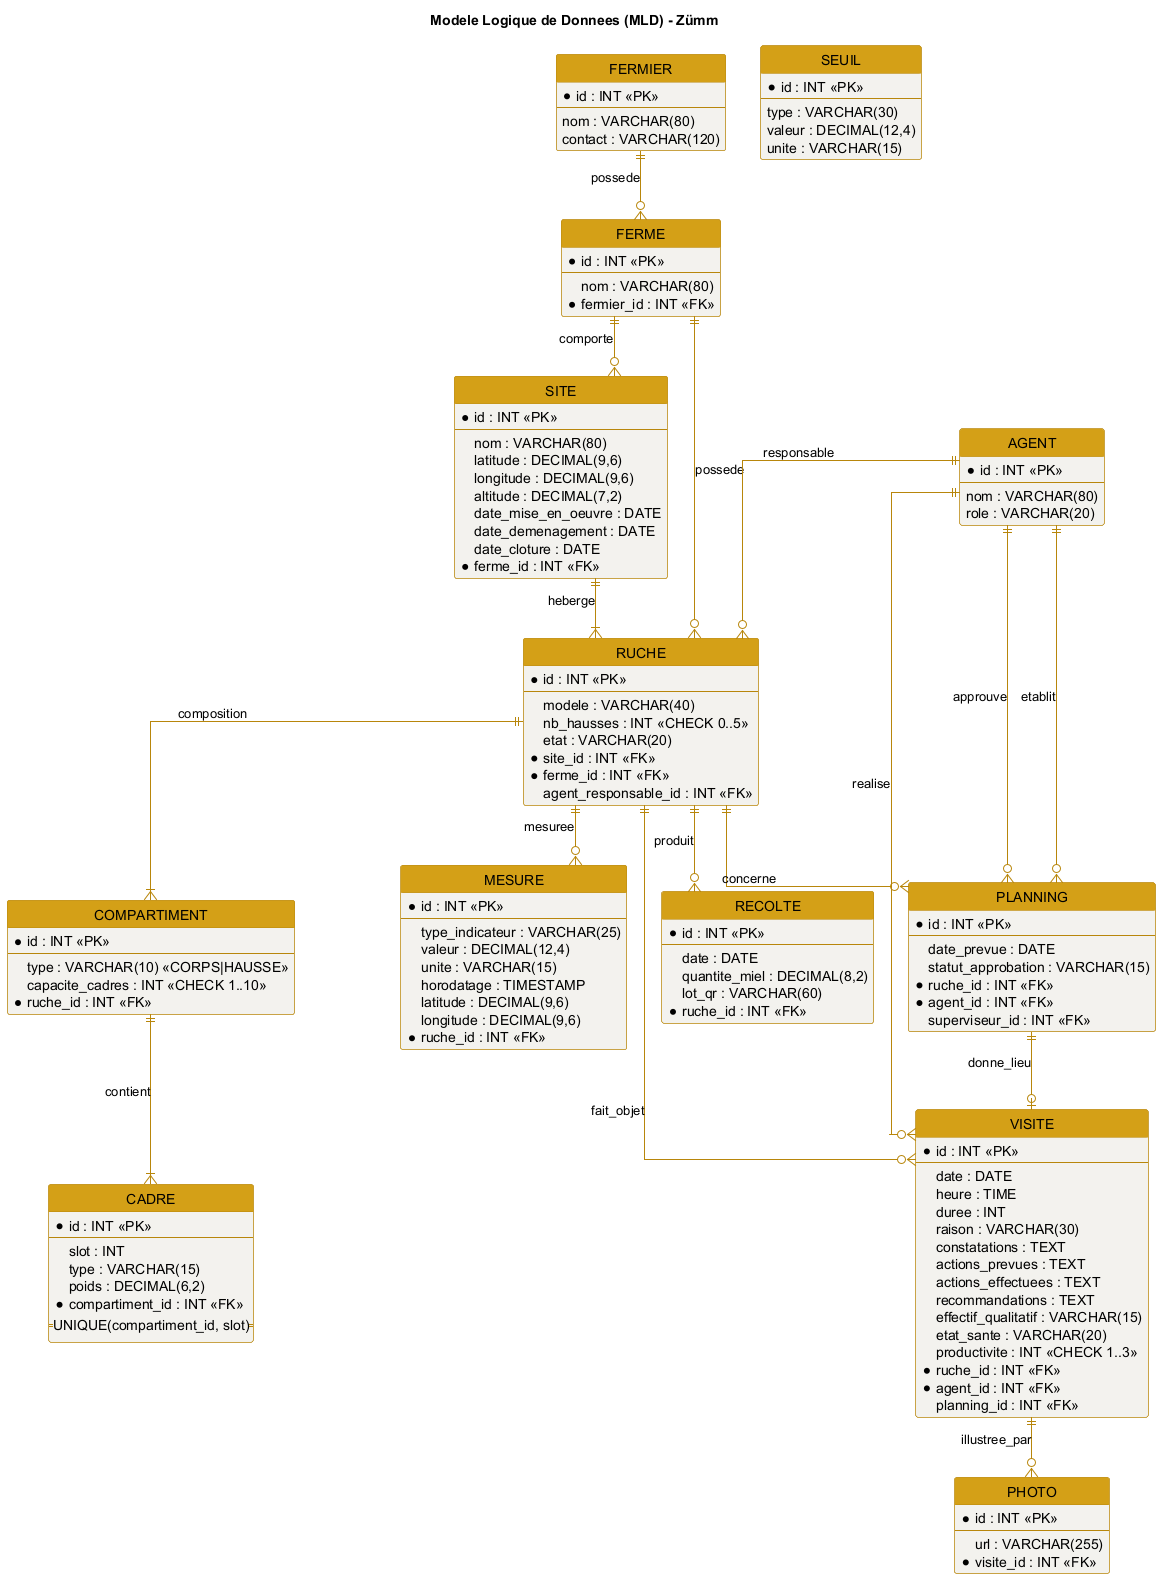
\includegraphics[width=0.82\linewidth]{diagramme_mld}
\caption{Modele logique de donnees relationnel du systeme Z\"umm.}
\label{fig:mld}
\end{figure}

%------------------------------------------------------------------------------
\section{Maquettes de l'interface (wireframes)}
%------------------------------------------------------------------------------
Les maquettes basse-fidelite suivantes fixent l'ergonomie des ecrans cles avant
le developpement. Elles respectent la charte visuelle et la simplicite exigee.

\begin{figure}[htbp]
\centering
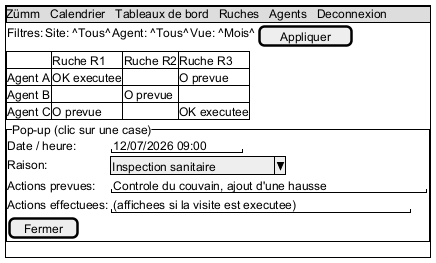
\includegraphics[width=0.9\linewidth]{wireframe_calendrier}
\caption{Maquette : calendrier / matrice agents x ruches avec pop-up de visite.}
\label{fig:wf-calendrier}
\end{figure}

\begin{figure}[htbp]
\centering
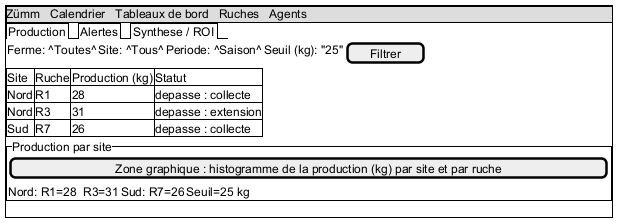
\includegraphics[width=0.9\linewidth]{wireframe_tdb_production}
\caption{Maquette : tableau de bord de production avec seuil parametrable.}
\label{fig:wf-production}
\end{figure}

\begin{figure}[htbp]
\centering
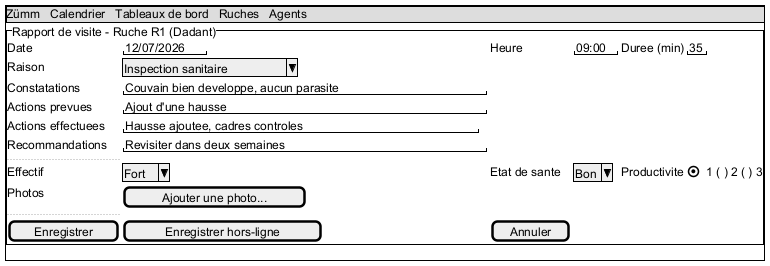
\includegraphics[width=0.95\linewidth]{wireframe_rapport_visite}
\caption{Maquette : formulaire de rapport de visite (avec mode hors-ligne et photos).}
\label{fig:wf-rapport}
\end{figure}

\begin{figure}[htbp]
\centering
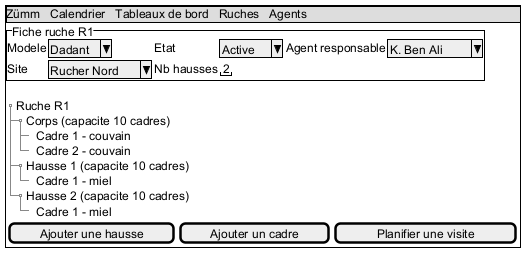
\includegraphics[width=0.85\linewidth]{wireframe_ruche}
\caption{Maquette : fiche d'une ruche et composition (corps, hausses, cadres).}
\label{fig:wf-ruche}
\end{figure}

%------------------------------------------------------------------------------
\section{Matrice des droits d'acces (RBAC)}
%------------------------------------------------------------------------------
La matrice precise, pour chaque fonction, le droit accorde a chaque profil.
\textbf{Legende :} CRUD = creation / lecture / mise a jour / suppression ;
R = lecture ; X = execution ; A = approbation ; --- = aucun acces.

\begin{longtable}{>{\bfseries}p{3.6cm} C{1.3cm} C{1.3cm} C{1.3cm} C{1.3cm} C{1.3cm} C{1.3cm}}
\toprule
\textbf{Fonction} & \textbf{Prop.} & \textbf{Apic.} & \textbf{Sup.} & \textbf{Resp.} & \textbf{Admin} & \textbf{API} \\
\midrule
\endhead
Fermes et sites          & CRUD & R    & R    & R    & CRUD & --- \\
Ruches (corps/cadres)    & CRUD & R    & R    & R    & CRUD & --- \\
Agents                   & R    & ---  & R    & R    & CRUD & --- \\
Planifier une visite     & R    & X    & X    & X    & X    & --- \\
Approuver le planning    & ---  & ---  & A    & ---  & X    & --- \\
Realiser visite/rapport  & R    & X    & X    & ---  & R    & --- \\
Calendrier agents x ruches & R  & R    & R    & R    & R    & --- \\
TB production            & R    & ---  & ---  & R    & R    & --- \\
TB alertes / traiter     & R    & ---  & ---  & X    & R    & --- \\
Synthese et ROI          & R    & ---  & ---  & R    & R    & --- \\
Parametrer seuils/unites & ---  & ---  & ---  & R    & CRUD & --- \\
Internationalisation     & ---  & ---  & ---  & ---  & CRUD & --- \\
Export CSV / TXT         & R    & R    & R    & R    & R    & --- \\
Sauvegarde / restauration & --- & ---  & ---  & ---  & X    & --- \\
API quantite de miel     & ---  & ---  & ---  & ---  & ---  & R \\
\bottomrule
\end{longtable}

\begin{encadre}
Cette matrice doit etre appliquee cote serveur (verification systematique des
droits dans la couche de controle), et non uniquement par le masquage des
elements d'interface.
\end{encadre}

%------------------------------------------------------------------------------
\section{Registre des risques}
%------------------------------------------------------------------------------
\begin{longtable}{>{\bfseries}p{4.6cm} C{1.8cm} C{1.6cm} p{5.4cm}}
\toprule
\textbf{Risque} & \textbf{Probab.} & \textbf{Impact} & \textbf{Mesure de reduction} \\
\midrule
\endhead
Retard de developpement       & Moyenne & Fort      & Prioriser le noyau CRUD ; jalons hebdomadaires (S5 a S12). \\
Portee trop large             & Moyenne & Fort      & Se limiter aux fonctions de priorite haute ; le reste en option. \\
Complexite i18n arabe (RTL)   & Moyenne & Moyen     & Test precoce de bout en bout FR/EN/AR, gestion \texttt{dir=rtl}. \\
Perte de donnees terrain      & Moyenne & Fort      & File de commandes hors-ligne + synchronisation + sauvegarde. \\
Failles applicatives (injection, XSS) & Moyenne & Fort & \texttt{PreparedStatement}, echappement JSP, revue de securite. \\
Fausses alertes (capteurs)    & Moyenne & Moyen     & Seuils parametrables + validation humaine par le rapport. \\
Indisponibilite d'OAuth Google & Faible & Moyen     & Repli d'authentification locale pour la demonstration. \\
Volumetrie des mesures        & Faible  & Moyen     & Archivage et agregation par periode (volet automatise). \\
Usage d'un generateur de code & Faible  & Tres fort & Conception et code faits maison, tracabilite et revue par pairs. \\
\bottomrule
\end{longtable}

%------------------------------------------------------------------------------
\section{Protection des donnees personnelles}
%------------------------------------------------------------------------------
Le systeme manipule des donnees personnelles (noms et contacts des fermiers et
des agents) et des donnees potentiellement sensibles (\textbf{geolocalisation}
precise des sites). Les principes suivants sont retenus, dans l'esprit du RGPD :
\begin{itemize}
  \item \textbf{Minimisation et finalite} : ne collecter que les donnees utiles au suivi apicole.
  \item \textbf{Securite} : chiffrement des echanges (SSL / X.509) et acces authentifies, deja prevus.
  \item \textbf{Controle d'acces} : application stricte de la matrice RBAC ci-dessus.
  \item \textbf{Droits des personnes} : consultation, rectification et \textbf{effacement} des donnees, \textbf{portabilite} assuree par l'export CSV / TXT.
  \item \textbf{Conservation} : duree de retention definie pour les mesures et les visites, au-dela de laquelle les donnees sont archivees ou anonymisees.
  \item \textbf{Tracabilite} : journalisation des acces et des actions sensibles (approbation de planning, cloture de site).
\end{itemize}

%------------------------------------------------------------------------------
\section{Strategie de tests}
%------------------------------------------------------------------------------
La strategie complete le plan de tests fonctionnels (chapitre~10) par les
niveaux unitaire et d'integration. La conception faiblement couplee (interfaces
\texttt{Repository}, services segreges) rend les regles metier testables en
isolation, par injection de doubles (mocks).

\begin{longtable}{>{\bfseries}p{2.8cm} p{4.4cm} p{4.4cm} C{2.2cm}}
\toprule
\textbf{Niveau} & \textbf{Portee} & \textbf{Exemples} & \textbf{Outil} \\
\midrule
\endhead
Unitaire      & Regles de gestion isolees          & Contraintes cadres/hausses, calcul du miel (Composite), ROI, seuils & JUnit 5, Mockito \\
Integration   & Acces aux donnees (Repository/JDBC) & CRUD persiste, requetes de calcul                                   & JUnit + base H2 \\
Systeme       & Cas fonctionnels de bout en bout    & Cas TC01 a TC16 du chapitre~10                                      & JUnit, Selenium \\
Acceptation   & Validation par la demonstration     & Parcours agent, fermier, responsable                                & Soutenance \\
\bottomrule
\end{longtable}

\begin{itemize}
  \item \textbf{Couverture visee} : au moins 70\,\% de la couche metier (regles de gestion), mesuree par \texttt{JaCoCo}.
  \item \textbf{Tracabilite} : chaque exigence est reliee a au moins un cas de test (matrice du chapitre~10), completee par les tests unitaires correspondants.
  \item \textbf{Automatisation} : execution des tests a chaque build (Maven), pre-requis a la livraison.
\end{itemize}

\begin{encadre}
\textbf{Synergie avec la conception :} l'inversion de dependance (DIP) permet de
substituer un \texttt{RucheRepository} en memoire aux implementations JDBC, ce
qui rend les tests rapides, deterministes et independants de la base.
\end{encadre}


\end{document}
